% Options for packages loaded elsewhere
\PassOptionsToPackage{unicode}{hyperref}
\PassOptionsToPackage{hyphens}{url}
\PassOptionsToPackage{dvipsnames,svgnames,x11names}{xcolor}
%
\documentclass[
  letterpaper,
  DIV=11,
  numbers=noendperiod]{scrreprt}

\usepackage{amsmath,amssymb}
\usepackage{iftex}
\ifPDFTeX
  \usepackage[T1]{fontenc}
  \usepackage[utf8]{inputenc}
  \usepackage{textcomp} % provide euro and other symbols
\else % if luatex or xetex
  \usepackage{unicode-math}
  \defaultfontfeatures{Scale=MatchLowercase}
  \defaultfontfeatures[\rmfamily]{Ligatures=TeX,Scale=1}
\fi
\usepackage{lmodern}
\ifPDFTeX\else  
    % xetex/luatex font selection
\fi
% Use upquote if available, for straight quotes in verbatim environments
\IfFileExists{upquote.sty}{\usepackage{upquote}}{}
\IfFileExists{microtype.sty}{% use microtype if available
  \usepackage[]{microtype}
  \UseMicrotypeSet[protrusion]{basicmath} % disable protrusion for tt fonts
}{}
\makeatletter
\@ifundefined{KOMAClassName}{% if non-KOMA class
  \IfFileExists{parskip.sty}{%
    \usepackage{parskip}
  }{% else
    \setlength{\parindent}{0pt}
    \setlength{\parskip}{6pt plus 2pt minus 1pt}}
}{% if KOMA class
  \KOMAoptions{parskip=half}}
\makeatother
\usepackage{xcolor}
\setlength{\emergencystretch}{3em} % prevent overfull lines
\setcounter{secnumdepth}{5}
% Make \paragraph and \subparagraph free-standing
\ifx\paragraph\undefined\else
  \let\oldparagraph\paragraph
  \renewcommand{\paragraph}[1]{\oldparagraph{#1}\mbox{}}
\fi
\ifx\subparagraph\undefined\else
  \let\oldsubparagraph\subparagraph
  \renewcommand{\subparagraph}[1]{\oldsubparagraph{#1}\mbox{}}
\fi

\usepackage{color}
\usepackage{fancyvrb}
\newcommand{\VerbBar}{|}
\newcommand{\VERB}{\Verb[commandchars=\\\{\}]}
\DefineVerbatimEnvironment{Highlighting}{Verbatim}{commandchars=\\\{\}}
% Add ',fontsize=\small' for more characters per line
\usepackage{framed}
\definecolor{shadecolor}{RGB}{241,243,245}
\newenvironment{Shaded}{\begin{snugshade}}{\end{snugshade}}
\newcommand{\AlertTok}[1]{\textcolor[rgb]{0.68,0.00,0.00}{#1}}
\newcommand{\AnnotationTok}[1]{\textcolor[rgb]{0.37,0.37,0.37}{#1}}
\newcommand{\AttributeTok}[1]{\textcolor[rgb]{0.40,0.45,0.13}{#1}}
\newcommand{\BaseNTok}[1]{\textcolor[rgb]{0.68,0.00,0.00}{#1}}
\newcommand{\BuiltInTok}[1]{\textcolor[rgb]{0.00,0.23,0.31}{#1}}
\newcommand{\CharTok}[1]{\textcolor[rgb]{0.13,0.47,0.30}{#1}}
\newcommand{\CommentTok}[1]{\textcolor[rgb]{0.37,0.37,0.37}{#1}}
\newcommand{\CommentVarTok}[1]{\textcolor[rgb]{0.37,0.37,0.37}{\textit{#1}}}
\newcommand{\ConstantTok}[1]{\textcolor[rgb]{0.56,0.35,0.01}{#1}}
\newcommand{\ControlFlowTok}[1]{\textcolor[rgb]{0.00,0.23,0.31}{#1}}
\newcommand{\DataTypeTok}[1]{\textcolor[rgb]{0.68,0.00,0.00}{#1}}
\newcommand{\DecValTok}[1]{\textcolor[rgb]{0.68,0.00,0.00}{#1}}
\newcommand{\DocumentationTok}[1]{\textcolor[rgb]{0.37,0.37,0.37}{\textit{#1}}}
\newcommand{\ErrorTok}[1]{\textcolor[rgb]{0.68,0.00,0.00}{#1}}
\newcommand{\ExtensionTok}[1]{\textcolor[rgb]{0.00,0.23,0.31}{#1}}
\newcommand{\FloatTok}[1]{\textcolor[rgb]{0.68,0.00,0.00}{#1}}
\newcommand{\FunctionTok}[1]{\textcolor[rgb]{0.28,0.35,0.67}{#1}}
\newcommand{\ImportTok}[1]{\textcolor[rgb]{0.00,0.46,0.62}{#1}}
\newcommand{\InformationTok}[1]{\textcolor[rgb]{0.37,0.37,0.37}{#1}}
\newcommand{\KeywordTok}[1]{\textcolor[rgb]{0.00,0.23,0.31}{#1}}
\newcommand{\NormalTok}[1]{\textcolor[rgb]{0.00,0.23,0.31}{#1}}
\newcommand{\OperatorTok}[1]{\textcolor[rgb]{0.37,0.37,0.37}{#1}}
\newcommand{\OtherTok}[1]{\textcolor[rgb]{0.00,0.23,0.31}{#1}}
\newcommand{\PreprocessorTok}[1]{\textcolor[rgb]{0.68,0.00,0.00}{#1}}
\newcommand{\RegionMarkerTok}[1]{\textcolor[rgb]{0.00,0.23,0.31}{#1}}
\newcommand{\SpecialCharTok}[1]{\textcolor[rgb]{0.37,0.37,0.37}{#1}}
\newcommand{\SpecialStringTok}[1]{\textcolor[rgb]{0.13,0.47,0.30}{#1}}
\newcommand{\StringTok}[1]{\textcolor[rgb]{0.13,0.47,0.30}{#1}}
\newcommand{\VariableTok}[1]{\textcolor[rgb]{0.07,0.07,0.07}{#1}}
\newcommand{\VerbatimStringTok}[1]{\textcolor[rgb]{0.13,0.47,0.30}{#1}}
\newcommand{\WarningTok}[1]{\textcolor[rgb]{0.37,0.37,0.37}{\textit{#1}}}

\providecommand{\tightlist}{%
  \setlength{\itemsep}{0pt}\setlength{\parskip}{0pt}}\usepackage{longtable,booktabs,array}
\usepackage{calc} % for calculating minipage widths
% Correct order of tables after \paragraph or \subparagraph
\usepackage{etoolbox}
\makeatletter
\patchcmd\longtable{\par}{\if@noskipsec\mbox{}\fi\par}{}{}
\makeatother
% Allow footnotes in longtable head/foot
\IfFileExists{footnotehyper.sty}{\usepackage{footnotehyper}}{\usepackage{footnote}}
\makesavenoteenv{longtable}
\usepackage{graphicx}
\makeatletter
\def\maxwidth{\ifdim\Gin@nat@width>\linewidth\linewidth\else\Gin@nat@width\fi}
\def\maxheight{\ifdim\Gin@nat@height>\textheight\textheight\else\Gin@nat@height\fi}
\makeatother
% Scale images if necessary, so that they will not overflow the page
% margins by default, and it is still possible to overwrite the defaults
% using explicit options in \includegraphics[width, height, ...]{}
\setkeys{Gin}{width=\maxwidth,height=\maxheight,keepaspectratio}
% Set default figure placement to htbp
\makeatletter
\def\fps@figure{htbp}
\makeatother

\usepackage{booktabs}
\usepackage{longtable}
\usepackage{array}
\usepackage{multirow}
\usepackage{wrapfig}
\usepackage{float}
\usepackage{colortbl}
\usepackage{pdflscape}
\usepackage{tabu}
\usepackage{threeparttable}
\usepackage{threeparttablex}
\usepackage[normalem]{ulem}
\usepackage{makecell}
\usepackage{xcolor}
\usepackage{makeidx}
\makeindex
\KOMAoption{captions}{tableheading}
\makeatletter
\makeatother
\makeatletter
\@ifpackageloaded{bookmark}{}{\usepackage{bookmark}}
\makeatother
\makeatletter
\@ifpackageloaded{caption}{}{\usepackage{caption}}
\AtBeginDocument{%
\ifdefined\contentsname
  \renewcommand*\contentsname{Table of contents}
\else
  \newcommand\contentsname{Table of contents}
\fi
\ifdefined\listfigurename
  \renewcommand*\listfigurename{List of Figures}
\else
  \newcommand\listfigurename{List of Figures}
\fi
\ifdefined\listtablename
  \renewcommand*\listtablename{List of Tables}
\else
  \newcommand\listtablename{List of Tables}
\fi
\ifdefined\figurename
  \renewcommand*\figurename{Figure}
\else
  \newcommand\figurename{Figure}
\fi
\ifdefined\tablename
  \renewcommand*\tablename{Table}
\else
  \newcommand\tablename{Table}
\fi
}
\@ifpackageloaded{float}{}{\usepackage{float}}
\floatstyle{ruled}
\@ifundefined{c@chapter}{\newfloat{codelisting}{h}{lop}}{\newfloat{codelisting}{h}{lop}[chapter]}
\floatname{codelisting}{Listing}
\newcommand*\listoflistings{\listof{codelisting}{List of Listings}}
\makeatother
\makeatletter
\@ifpackageloaded{caption}{}{\usepackage{caption}}
\@ifpackageloaded{subcaption}{}{\usepackage{subcaption}}
\makeatother
\makeatletter
\@ifpackageloaded{tcolorbox}{}{\usepackage[skins,breakable]{tcolorbox}}
\makeatother
\makeatletter
\@ifundefined{shadecolor}{\definecolor{shadecolor}{rgb}{.97, .97, .97}}
\makeatother
\makeatletter
\makeatother
\makeatletter
\makeatother
\ifLuaTeX
  \usepackage{selnolig}  % disable illegal ligatures
\fi
\IfFileExists{bookmark.sty}{\usepackage{bookmark}}{\usepackage{hyperref}}
\IfFileExists{xurl.sty}{\usepackage{xurl}}{} % add URL line breaks if available
\urlstyle{same} % disable monospaced font for URLs
\hypersetup{
  pdftitle={Longitudinal Tutorial},
  pdfauthor={Anarina Murillo, Yingxi Kong, Monica Colon Vargas},
  colorlinks=true,
  linkcolor={blue},
  filecolor={Maroon},
  citecolor={Blue},
  urlcolor={Blue},
  pdfcreator={LaTeX via pandoc}}

\title{Longitudinal Tutorial}
\author{Anarina Murillo, Yingxi Kong, Monica Colon Vargas}
\date{2024-07-08}

\begin{document}
\maketitle
\ifdefined\Shaded\renewenvironment{Shaded}{\begin{tcolorbox}[sharp corners, interior hidden, borderline west={3pt}{0pt}{shadecolor}, breakable, enhanced, boxrule=0pt, frame hidden]}{\end{tcolorbox}}\fi

\renewcommand*\contentsname{Table of contents}
{
\hypersetup{linkcolor=}
\setcounter{tocdepth}{2}
\tableofcontents
}
\bookmarksetup{startatroot}

\hypertarget{welcome}{%
\chapter*{Welcome}\label{welcome}}
\addcontentsline{toc}{chapter}{Welcome}

\markboth{Welcome}{Welcome}

This book gives an overview of longitudinal data analysis

\bookmarksetup{startatroot}

\hypertarget{preface}{%
\chapter*{Preface}\label{preface}}
\addcontentsline{toc}{chapter}{Preface}

\markboth{Preface}{Preface}

\part{Longitudinal Data Analysis}

\hypertarget{data-structure}{%
\section*{Data Structure}\label{data-structure}}
\addcontentsline{toc}{section}{Data Structure}

\markright{Data Structure}

\begin{Shaded}
\begin{Highlighting}[]
\FunctionTok{suppressPackageStartupMessages}\NormalTok{(}\FunctionTok{library}\NormalTok{(tidyr))}
\FunctionTok{suppressPackageStartupMessages}\NormalTok{(}\FunctionTok{library}\NormalTok{(data.table))}
\FunctionTok{suppressPackageStartupMessages}\NormalTok{(}\FunctionTok{library}\NormalTok{(ggplot2))}
\FunctionTok{suppressPackageStartupMessages}\NormalTok{(}\FunctionTok{library}\NormalTok{(haven))}
\FunctionTok{suppressPackageStartupMessages}\NormalTok{(}\FunctionTok{library}\NormalTok{(dplyr))}
\FunctionTok{suppressPackageStartupMessages}\NormalTok{(}\FunctionTok{library}\NormalTok{(GGally))}
\FunctionTok{suppressPackageStartupMessages}\NormalTok{(}\FunctionTok{library}\NormalTok{(kableExtra))}
\end{Highlighting}
\end{Shaded}

The most important part of any statistical analysis begins with loading
the data into Rstudio. Data can come in many forms with two popular ones
being csv (comma separated values) and dta. Below we show different
methods for how to load the data into RStudio.

\hypertarget{loading-csv-files}{%
\subsection*{Loading CSV files}\label{loading-csv-files}}
\addcontentsline{toc}{subsection}{Loading CSV files}

\hypertarget{using-base-r}{%
\subsubsection*{Using base R}\label{using-base-r}}
\addcontentsline{toc}{subsubsection}{Using base R}

The following method is a pretty standard way of loading csv files into
R. It requires no external packages (this is already a base R function)
and works as follows. First, specify the location of your data, and put
it into function as an input.

\begin{Shaded}
\begin{Highlighting}[]
\NormalTok{TLC }\OtherTok{\textless{}{-}} \FunctionTok{read.csv}\NormalTok{(}\StringTok{"Data/TLC.csv"}\NormalTok{)}
\end{Highlighting}
\end{Shaded}

We can then get a look at the data by using the head function which
provides us with a sneak peek of the first n rows.

\begin{Shaded}
\begin{Highlighting}[]
\FunctionTok{head}\NormalTok{(TLC, }\AttributeTok{n =} \DecValTok{10}\NormalTok{)}
\end{Highlighting}
\end{Shaded}

\begin{verbatim}
   id lead0 lead1 lead4 lead6     group
1   1  30.8  26.9  25.8  23.8   Placebo
2   2  26.5  14.8  19.5  21.0 Treatment
3   3  25.8  23.0  19.1  23.2 Treatment
4   4  24.7  24.5  22.0  22.5   Placebo
5   5  20.4   2.8   3.2   9.4 Treatment
6   6  20.4   5.4   4.5  11.9 Treatment
7   7  28.6  20.8  19.2  18.4   Placebo
8   8  33.7  31.6  28.5  25.1   Placebo
9   9  19.7  14.9  15.3  14.7   Placebo
10 10  31.1  31.2  29.2  30.1   Placebo
\end{verbatim}

\hypertarget{using-the-readr-package}{%
\subsubsection*{Using the readr package}\label{using-the-readr-package}}
\addcontentsline{toc}{subsubsection}{Using the readr package}

The next method requires the use of the readr package. It works exactly
the same as read.csv, save for the fact that it is faster than read.csv.

\begin{Shaded}
\begin{Highlighting}[]
\FunctionTok{library}\NormalTok{(readr)}
\NormalTok{TLC }\OtherTok{\textless{}{-}} \FunctionTok{read\_csv}\NormalTok{(}\StringTok{"Data/TLC.csv"}\NormalTok{)}
\end{Highlighting}
\end{Shaded}

We can also print the first few rows to take a look of our data using
function \texttt{head}, here we print the first 10 rows of the data.

\begin{Shaded}
\begin{Highlighting}[]
\FunctionTok{head}\NormalTok{(TLC, }\AttributeTok{n =} \DecValTok{10}\NormalTok{)}
\end{Highlighting}
\end{Shaded}

\begin{verbatim}
# A tibble: 10 x 6
      id lead0 lead1 lead4 lead6 group    
   <dbl> <dbl> <dbl> <dbl> <dbl> <chr>    
 1     1  30.8 26.9   25.8 23.8  Placebo  
 2     2  26.5 14.8   19.5 21    Treatment
 3     3  25.8 23     19.1 23.2  Treatment
 4     4  24.7 24.5   22   22.5  Placebo  
 5     5  20.4  2.8    3.2  9.40 Treatment
 6     6  20.4  5.40   4.5 11.9  Treatment
 7     7  28.6 20.8   19.2 18.4  Placebo  
 8     8  33.7 31.6   28.5 25.1  Placebo  
 9     9  19.7 14.9   15.3 14.7  Placebo  
10    10  31.1 31.2   29.2 30.1  Placebo  
\end{verbatim}

\hypertarget{using-the-data.table-package}{%
\subsubsection*{Using the data.table
package}\label{using-the-data.table-package}}
\addcontentsline{toc}{subsubsection}{Using the data.table package}

If we have large datasets, we can use the fread function in the
data.table package to read the data faster compared to the other methods
above, and we print the first 5 rows of the data.

\begin{Shaded}
\begin{Highlighting}[]
\FunctionTok{library}\NormalTok{(data.table)}
\NormalTok{TLC }\OtherTok{\textless{}{-}} \FunctionTok{fread}\NormalTok{(}\StringTok{"Data/TLC.csv"}\NormalTok{)}
\FunctionTok{head}\NormalTok{(TLC, }\AttributeTok{n =} \DecValTok{5}\NormalTok{)}
\end{Highlighting}
\end{Shaded}

\begin{verbatim}
      id lead0 lead1 lead4 lead6     group
   <int> <num> <num> <num> <num>    <char>
1:     1  30.8  26.9  25.8  23.8   Placebo
2:     2  26.5  14.8  19.5  21.0 Treatment
3:     3  25.8  23.0  19.1  23.2 Treatment
4:     4  24.7  24.5  22.0  22.5   Placebo
5:     5  20.4   2.8   3.2   9.4 Treatment
\end{verbatim}

\hypertarget{loading-dta-files}{%
\subsection*{Loading dta files}\label{loading-dta-files}}
\addcontentsline{toc}{subsection}{Loading dta files}

We can also read files in other formats from other software (STATA,
SPSS, SAS, etc). Here we will explore reading dta files which is used in
STATA software. In order to load these into Rstudio we need to use a
package known as haven. The haven package has a function known as
\texttt{read\_dta()} which serves a similar purpose as
\texttt{read.csv()}, \texttt{read\_csv()} and \texttt{fread()}.

\begin{Shaded}
\begin{Highlighting}[]
\NormalTok{TLCdta }\OtherTok{\textless{}{-}} \FunctionTok{read\_dta}\NormalTok{(}\StringTok{"Data/TLC.dta"}\NormalTok{)}
\FunctionTok{head}\NormalTok{(TLCdta, }\AttributeTok{n =} \DecValTok{15}\NormalTok{)}
\end{Highlighting}
\end{Shaded}

\begin{verbatim}
# A tibble: 15 x 6
      id lead0 lead1 lead4 lead6 group    
   <dbl> <dbl> <dbl> <dbl> <dbl> <chr>    
 1     1  30.8 26.9  25.8  23.8  Placebo  
 2     2  26.5 14.8  19.5  21    Treatment
 3     3  25.8 23    19.1  23.2  Treatment
 4     4  24.7 24.5  22    22.5  Placebo  
 5     5  20.4  2.80  3.20  9.40 Treatment
 6     6  20.4  5.40  4.5  11.9  Treatment
 7     7  28.6 20.8  19.2  18.4  Placebo  
 8     8  33.7 31.6  28.5  25.1  Placebo  
 9     9  19.7 14.9  15.3  14.7  Placebo  
10    10  31.1 31.2  29.2  30.1  Placebo  
11    11  19.8 17.5  20.5  27.5  Placebo  
12    12  24.8 23.1  24.6  30.9  Treatment
13    13  21.4 26.3  19.5  19    Placebo  
14    14  27.9  6.30 18.5  16.3  Treatment
15    15  21.1 20.3  18.4  20.8  Placebo  
\end{verbatim}

\hypertarget{sec-longi-EDA}{%
\chapter{Exploratory Data Analysis}\label{sec-longi-EDA}}

\textbf{Learning Objectives}

\begin{enumerate}
\def\labelenumi{\arabic{enumi}.}
\item
  Understand how to conduct exploratory data analysis for longitudinal
  data.
\item
  Understand how to create plots to visualize trends over time and
  interpret results.
\item
  Understand how to calculate descriptive statistics (mean, standard
  deviation, variance-covariance matrix, correlation matrix) and
  interpret results.
\item
  Understand how to identify characteristics of longitudinal data.
\end{enumerate}

\hypertarget{converting-between-data-formats-wide-and-long-format}{%
\section{Converting between data formats (wide and long
format)}\label{converting-between-data-formats-wide-and-long-format}}

For the most part there are two formats that your data can come in. The
wide format and the long format. The long format is when patients within
the data have more than one observation. In other words, each row is
snapshot into a subject's history at a specific time point. In the case
of our data, each subject has four observations corresponding to their
four lead measurements (initial measurement, 1 week measurement, 4 week
measurement, and 6 week measurement). The code below details how to
convert from wide format to long format.

The arguments to \texttt{gather()}:

\begin{itemize}
\tightlist
\item
  \texttt{data}: Data object (e.g.~the data object here is TLC).
\item
  \texttt{key}: Name of new key column (made from names of data
  columns).
\item
  \texttt{value}: Name of new value column.
\item
  \texttt{...}: Names of source columns that contain values.
\item
  \texttt{factor\_key}: Treat the new key column as a factor (instead of
  character vector).
\end{itemize}

Then, we print the first 16 rows of the long format TLC data.

\begin{Shaded}
\begin{Highlighting}[]
\NormalTok{long\_TLC }\OtherTok{\textless{}{-}}\NormalTok{ tidyr}\SpecialCharTok{::}\FunctionTok{gather}\NormalTok{(TLC, level, measurements, lead0}\SpecialCharTok{:}\NormalTok{lead6, }\AttributeTok{factor\_key =} \ConstantTok{TRUE}\NormalTok{)}
\NormalTok{long\_TLC }\OtherTok{\textless{}{-}}\NormalTok{ long\_TLC[}\FunctionTok{order}\NormalTok{(long\_TLC}\SpecialCharTok{$}\NormalTok{id), ]}
\FunctionTok{head}\NormalTok{(long\_TLC, }\AttributeTok{n =} \DecValTok{16}\NormalTok{)}
\end{Highlighting}
\end{Shaded}

\begin{verbatim}
    id     group level measurements
1    1   Placebo lead0         30.8
101  1   Placebo lead1         26.9
201  1   Placebo lead4         25.8
301  1   Placebo lead6         23.8
2    2 Treatment lead0         26.5
102  2 Treatment lead1         14.8
202  2 Treatment lead4         19.5
302  2 Treatment lead6         21.0
3    3 Treatment lead0         25.8
103  3 Treatment lead1         23.0
203  3 Treatment lead4         19.1
303  3 Treatment lead6         23.2
4    4   Placebo lead0         24.7
104  4   Placebo lead1         24.5
204  4   Placebo lead4         22.0
304  4   Placebo lead6         22.5
\end{verbatim}

The wide format is when each row corresponds to a unique subject. The
below shows one how to convert from long format to wide.

The arguments to \texttt{spread()}:

\begin{itemize}
\tightlist
\item
  \texttt{data}: Data object.
\item
  \texttt{key}: Name of column containing the new column names.
\item
  \texttt{value}: Name of column containing values.
\end{itemize}

Then, we print the first 10 rows of the converted wide format TLC data
which should be same as our original data.

\begin{Shaded}
\begin{Highlighting}[]
\NormalTok{wide\_TLC }\OtherTok{\textless{}{-}} \FunctionTok{spread}\NormalTok{(long\_TLC, level, measurements)}
\FunctionTok{head}\NormalTok{(wide\_TLC, }\AttributeTok{n =} \DecValTok{10}\NormalTok{)}
\end{Highlighting}
\end{Shaded}

\begin{verbatim}
   id     group lead0 lead1 lead4 lead6
1   1   Placebo  30.8  26.9  25.8  23.8
2   2 Treatment  26.5  14.8  19.5  21.0
3   3 Treatment  25.8  23.0  19.1  23.2
4   4   Placebo  24.7  24.5  22.0  22.5
5   5 Treatment  20.4   2.8   3.2   9.4
6   6 Treatment  20.4   5.4   4.5  11.9
7   7   Placebo  28.6  20.8  19.2  18.4
8   8   Placebo  33.7  31.6  28.5  25.1
9   9   Placebo  19.7  14.9  15.3  14.7
10 10   Placebo  31.1  31.2  29.2  30.1
\end{verbatim}

\hypertarget{graphical-representation-of-longitudinal-data}{%
\section{Graphical Representation of Longitudinal
Data}\label{graphical-representation-of-longitudinal-data}}

In this section we will create some visual representations of the data.
While this is possible to do in base R, we will use ggplot. The plots
look nicer and it is a reliable tool for making data visualizations. We
will begin by plotting the blood lead level (BLL) trajectories for the
first seven subjects.

\hypertarget{individual-trajectory-plot}{%
\subsection{Individual Trajectory
Plot}\label{individual-trajectory-plot}}

We need to utilize \texttt{ggplot} package to graph the individual
trajectory plot. Before that, we firstly make some modification on our
data. We create a new numeric column named \texttt{time} corresponding
to the \texttt{level} column which represents the number of weeks for
the measurement as our x-axis timing variable. Next, we convert the
\texttt{id} column into factor so we can have each individual as a
group.

\begin{Shaded}
\begin{Highlighting}[]
\CommentTok{\# create a new numeric timing variable}
\NormalTok{long\_TLC}\SpecialCharTok{$}\NormalTok{time }\OtherTok{\textless{}{-}} \FunctionTok{c}\NormalTok{(}\DecValTok{0}\NormalTok{, }\DecValTok{1}\NormalTok{, }\DecValTok{4}\NormalTok{, }\DecValTok{6}\NormalTok{)[long\_TLC}\SpecialCharTok{$}\NormalTok{level]}

\CommentTok{\# convert the id column into factor for grouping}
\NormalTok{long\_TLC}\SpecialCharTok{$}\NormalTok{id }\OtherTok{\textless{}{-}} \FunctionTok{as.factor}\NormalTok{(long\_TLC}\SpecialCharTok{$}\NormalTok{id)}
\end{Highlighting}
\end{Shaded}

Next, we are reading to graph the individual trajectory plot, and we
only focus on the first 7 id's individual.

\begin{Shaded}
\begin{Highlighting}[]
\CommentTok{\# create plot}
\NormalTok{lead\_trajectories }\OtherTok{\textless{}{-}} \FunctionTok{ggplot}\NormalTok{(}\AttributeTok{data =}\NormalTok{ long\_TLC[(long\_TLC[,}\StringTok{"id"}\NormalTok{] }\SpecialCharTok{\%in\%} \DecValTok{1}\SpecialCharTok{:}\DecValTok{7}\NormalTok{), ]) }\SpecialCharTok{+} \CommentTok{\#only focus on id\textquotesingle{}s 1{-}7}
  \FunctionTok{geom\_line}\NormalTok{(}\FunctionTok{aes}\NormalTok{(}\AttributeTok{x =}\NormalTok{ time, }\AttributeTok{y =}\NormalTok{ measurements, }\AttributeTok{color =}\NormalTok{ id, }\AttributeTok{group =}\NormalTok{ id),}\AttributeTok{size =} \FloatTok{1.7}\NormalTok{) }\SpecialCharTok{+} 
  \FunctionTok{theme}\NormalTok{(}\AttributeTok{axis.line =} \FunctionTok{element\_line}\NormalTok{(}\AttributeTok{colour =} \StringTok{"black"}\NormalTok{, }\AttributeTok{size =} \DecValTok{2}\NormalTok{),}
        \AttributeTok{text =} \FunctionTok{element\_text}\NormalTok{(}\AttributeTok{size =} \DecValTok{20}\NormalTok{),}
        \AttributeTok{axis.text =} \FunctionTok{element\_text}\NormalTok{(}\AttributeTok{colour =} \StringTok{"black"}\NormalTok{, }\AttributeTok{size =} \DecValTok{16}\NormalTok{, }\AttributeTok{face =} \StringTok{"bold"}\NormalTok{),}
        \AttributeTok{axis.title =} \FunctionTok{element\_text}\NormalTok{(}\AttributeTok{size =} \DecValTok{16}\NormalTok{, }\AttributeTok{face=}\StringTok{"bold"}\NormalTok{),}
        \AttributeTok{axis.ticks.length =} \FunctionTok{unit}\NormalTok{(.}\DecValTok{25}\NormalTok{, }\StringTok{"cm"}\NormalTok{),}
        \AttributeTok{axis.ticks =} \FunctionTok{element\_line}\NormalTok{(}\AttributeTok{colour =} \StringTok{"black"}\NormalTok{, }\AttributeTok{size =} \FloatTok{1.5}\NormalTok{),}
        \AttributeTok{legend.background =} \FunctionTok{element\_blank}\NormalTok{()) }\SpecialCharTok{+}
  \FunctionTok{scale\_color\_manual}\NormalTok{(}\AttributeTok{name =} \StringTok{"ID"}\NormalTok{, }\AttributeTok{values =} \FunctionTok{c}\NormalTok{(}\StringTok{"green"}\NormalTok{, }\StringTok{"red"}\NormalTok{, }\StringTok{"purple"}\NormalTok{, }\StringTok{"blue"}\NormalTok{,}
                                             \StringTok{"yellow"}\NormalTok{, }\StringTok{"pink"}\NormalTok{, }\StringTok{"orange"}\NormalTok{),}
                     \AttributeTok{labels =} \FunctionTok{sapply}\NormalTok{(}\DecValTok{1}\SpecialCharTok{:}\DecValTok{7}\NormalTok{, }\ControlFlowTok{function}\NormalTok{(x) }\FunctionTok{paste0}\NormalTok{(}\StringTok{"id"}\NormalTok{, }\StringTok{" = "}\NormalTok{, x))) }\SpecialCharTok{+}
  \FunctionTok{ylab}\NormalTok{(}\SpecialCharTok{\textasciitilde{}} \FunctionTok{paste}\NormalTok{(}\StringTok{"Blood Lead levels ("}\NormalTok{, mu, }\StringTok{"g/dL)"}\NormalTok{)) }\SpecialCharTok{+}
  \FunctionTok{xlab}\NormalTok{(}\StringTok{"Time (weeks)"}\NormalTok{)}

\CommentTok{\# print the individual trajectory plot}
\FunctionTok{print}\NormalTok{(lead\_trajectories)}
\end{Highlighting}
\end{Shaded}

\begin{figure}[H]

{\centering 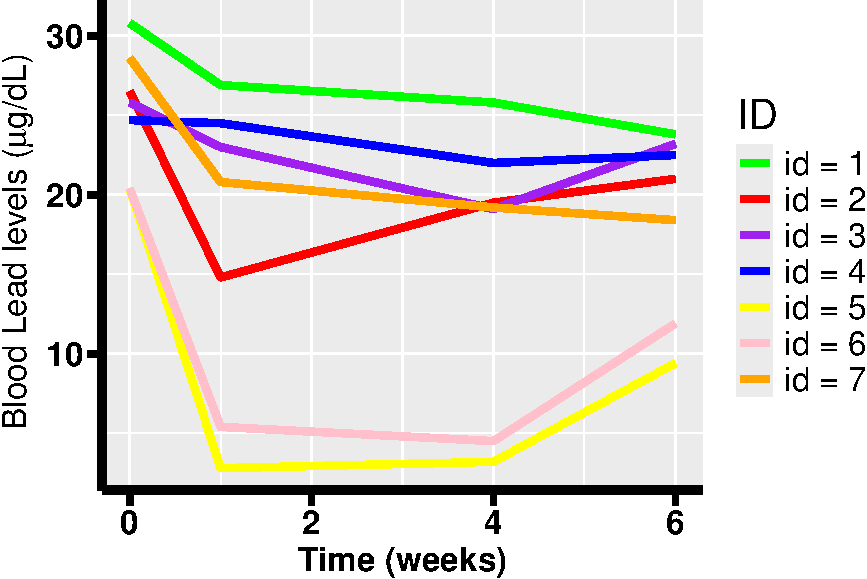
\includegraphics{Longi_EDA_files/figure-pdf/unnamed-chunk-6-1.pdf}

}

\end{figure}

\hypertarget{scatter-plot}{%
\subsection{Scatter Plot}\label{scatter-plot}}

Next, we create a scatter plot to evaluate BLL over time. We stratify
the data by group.

\begin{Shaded}
\begin{Highlighting}[]
\NormalTok{long\_TLC}\SpecialCharTok{$}\NormalTok{factor\_time }\OtherTok{\textless{}{-}} \FunctionTok{as.factor}\NormalTok{(long\_TLC}\SpecialCharTok{$}\NormalTok{time)}

\CommentTok{\#create plot}
\NormalTok{lead\_point\_plot }\OtherTok{\textless{}{-}} \FunctionTok{ggplot}\NormalTok{(long\_TLC, }
                          \FunctionTok{aes}\NormalTok{(}\AttributeTok{x =}\NormalTok{ factor\_time, }\AttributeTok{y =}\NormalTok{ measurements, }\AttributeTok{color =}\NormalTok{ group)) }\SpecialCharTok{+} 
  \FunctionTok{geom\_point}\NormalTok{() }\SpecialCharTok{+} 
  \FunctionTok{facet\_wrap}\NormalTok{(.}\SpecialCharTok{\textasciitilde{}}\NormalTok{group) }\SpecialCharTok{+} \CommentTok{\# this allows us to make separate boxes for the groups}
  \FunctionTok{theme}\NormalTok{(}\AttributeTok{axis.line =} \FunctionTok{element\_line}\NormalTok{(}\AttributeTok{colour =} \StringTok{"black"}\NormalTok{, }\AttributeTok{size =} \DecValTok{2}\NormalTok{),}
        \AttributeTok{text =} \FunctionTok{element\_text}\NormalTok{(}\AttributeTok{size =} \DecValTok{20}\NormalTok{),}
        \AttributeTok{axis.text =} \FunctionTok{element\_text}\NormalTok{(}\AttributeTok{colour =} \StringTok{"black"}\NormalTok{, }\AttributeTok{size =} \DecValTok{16}\NormalTok{, }\AttributeTok{face=}\StringTok{"bold"}\NormalTok{),}
        \AttributeTok{axis.title =} \FunctionTok{element\_text}\NormalTok{(}\AttributeTok{size =} \DecValTok{16}\NormalTok{, }\AttributeTok{face =} \StringTok{"bold"}\NormalTok{),}
        \AttributeTok{axis.ticks.length=}\FunctionTok{unit}\NormalTok{(.}\DecValTok{25}\NormalTok{, }\StringTok{"cm"}\NormalTok{),}
        \AttributeTok{axis.ticks =} \FunctionTok{element\_line}\NormalTok{(}\AttributeTok{colour =} \StringTok{"black"}\NormalTok{, }\AttributeTok{size =} \FloatTok{1.5}\NormalTok{)) }\SpecialCharTok{+} 
  \FunctionTok{ylab}\NormalTok{(}\SpecialCharTok{\textasciitilde{}} \FunctionTok{paste}\NormalTok{(}\StringTok{"Blood Lead levels ("}\NormalTok{, mu, }\StringTok{"g/dL)"}\NormalTok{)) }\SpecialCharTok{+} 
  \FunctionTok{xlab}\NormalTok{(}\StringTok{"Time (weeks)"}\NormalTok{)}

\CommentTok{\# print the scatter plot}
\FunctionTok{print}\NormalTok{(lead\_point\_plot)}
\end{Highlighting}
\end{Shaded}

\begin{figure}[H]

{\centering 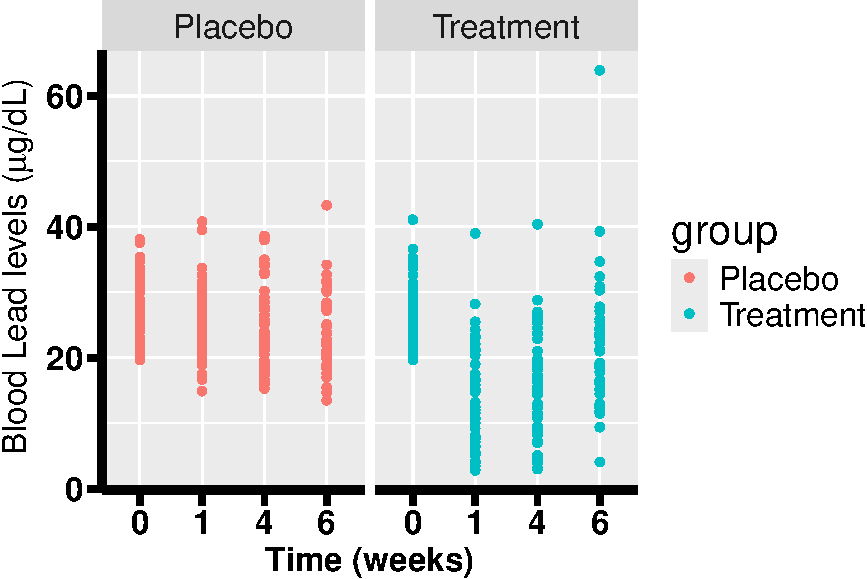
\includegraphics{Longi_EDA_files/figure-pdf/unnamed-chunk-7-1.pdf}

}

\end{figure}

\hypertarget{mean-plot}{%
\subsection{Mean Plot}\label{mean-plot}}

To plot averages over time, we first summarize the data. Here we
summarize count, mean, standard deviation (SD) and variance of blood
lead levels over time (or for each occasion).

\begin{Shaded}
\begin{Highlighting}[]
\CommentTok{\#create table summarizing the blood lead levels}
\NormalTok{lead\_overall\_summary }\OtherTok{\textless{}{-}}\NormalTok{ long\_TLC }\SpecialCharTok{\%\textgreater{}\%}
  \FunctionTok{group\_by}\NormalTok{(time) }\SpecialCharTok{\%\textgreater{}\%} \CommentTok{\#CHECK}
  \FunctionTok{summarise}\NormalTok{(}\AttributeTok{n =}\NormalTok{ (}\FunctionTok{length}\NormalTok{(measurements) }\SpecialCharTok{{-}} \FunctionTok{sum}\NormalTok{(}\FunctionTok{is.na}\NormalTok{(measurements))),}
            \AttributeTok{mean =} \FunctionTok{round}\NormalTok{(}\FunctionTok{mean}\NormalTok{(measurements, }\AttributeTok{na.rm =}\NormalTok{ T), }\DecValTok{3}\NormalTok{),}
            \AttributeTok{sd =} \FunctionTok{round}\NormalTok{(}\FunctionTok{sd}\NormalTok{(measurements, }\AttributeTok{na.rm =}\NormalTok{ T), }\DecValTok{3}\NormalTok{),}
            \AttributeTok{var =} \FunctionTok{round}\NormalTok{(}\FunctionTok{var}\NormalTok{(measurements, }\AttributeTok{na.rm =}\NormalTok{ T), }\DecValTok{3}\NormalTok{))}

\CommentTok{\#output table for overall averages}
\NormalTok{lead\_overall\_summary }\SpecialCharTok{\%\textgreater{}\%}
  \FunctionTok{mutate\_all}\NormalTok{(linebreak) }\SpecialCharTok{\%\textgreater{}\%}
  \FunctionTok{kbl}\NormalTok{(}\AttributeTok{caption =} \StringTok{"Summary of average lead levels from TLC study"}\NormalTok{,}
      \AttributeTok{col.names=}\FunctionTok{linebreak}\NormalTok{(}\FunctionTok{c}\NormalTok{(}\StringTok{"Time"}\NormalTok{,}\StringTok{"N"}\NormalTok{, }\StringTok{"Mean"}\NormalTok{, }\StringTok{"SD"}\NormalTok{, }\StringTok{"Variance"}\NormalTok{)),}
      \AttributeTok{booktabs=}\NormalTok{T, }\AttributeTok{escape=}\NormalTok{F, }\AttributeTok{align =} \StringTok{"c"}\NormalTok{) }\SpecialCharTok{\%\textgreater{}\%}
  \FunctionTok{kable\_styling}\NormalTok{(}\AttributeTok{full\_width =} \ConstantTok{FALSE}\NormalTok{, }\AttributeTok{latex\_options =} \FunctionTok{c}\NormalTok{(}\StringTok{\textquotesingle{}hold\_position\textquotesingle{}}\NormalTok{))}
\end{Highlighting}
\end{Shaded}

\begin{table}[!h]
\centering
\caption{Summary of average lead levels from TLC study}
\centering
\begin{tabular}[t]{ccccc}
\toprule
Time & N & Mean & SD & Variance\\
\midrule
0 & 100 & 26.406 & 4.999 & 24.989\\
1 & 100 & 19.091 & 8.673 & 75.225\\
4 & 100 & 19.792 & 8.086 & 65.385\\
6 & 100 & 22.204 & 7.756 & 60.159\\
\bottomrule
\end{tabular}
\end{table}

Next, we create a plot of means.

\begin{Shaded}
\begin{Highlighting}[]
\NormalTok{lead\_mean\_plot }\OtherTok{\textless{}{-}} \FunctionTok{ggplot}\NormalTok{(}\AttributeTok{data =}\NormalTok{ lead\_overall\_summary, }\FunctionTok{aes}\NormalTok{(}\AttributeTok{x =}\NormalTok{ time, }\AttributeTok{y =}\NormalTok{ mean)) }\SpecialCharTok{+}
    \FunctionTok{geom\_point}\NormalTok{(}\AttributeTok{size =} \DecValTok{2}\NormalTok{) }\SpecialCharTok{+} \FunctionTok{geom\_line}\NormalTok{(}\AttributeTok{size =} \DecValTok{2}\NormalTok{) }\SpecialCharTok{+} \FunctionTok{ylab}\NormalTok{(}\SpecialCharTok{\textasciitilde{}}\FunctionTok{paste}\NormalTok{(}\StringTok{"Lead levels ("}\NormalTok{, mu,}
    \StringTok{"g/dL)"}\NormalTok{)) }\SpecialCharTok{+} \FunctionTok{xlab}\NormalTok{(}\StringTok{"Time (weeks)"}\NormalTok{)}

\CommentTok{\# print the mean plot}
\FunctionTok{print}\NormalTok{(lead\_mean\_plot)}
\end{Highlighting}
\end{Shaded}

\begin{figure}[H]

{\centering 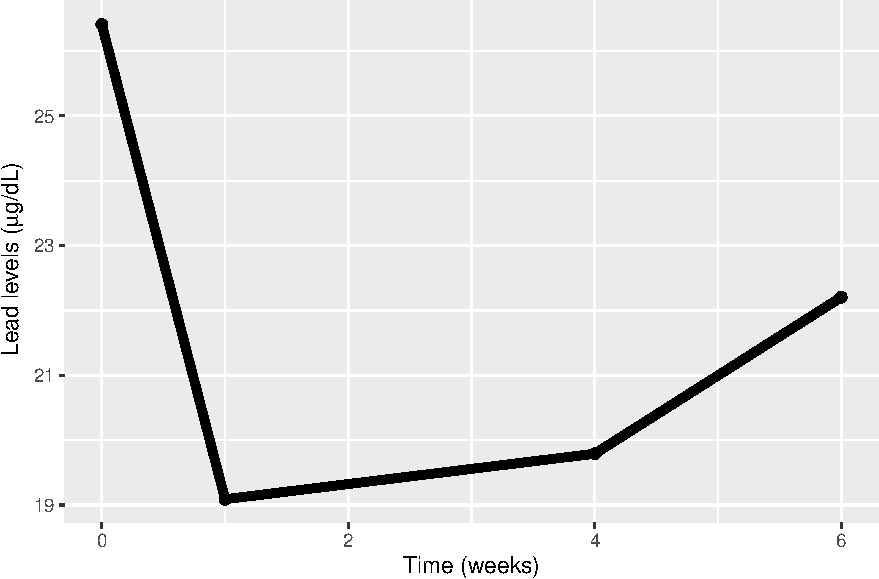
\includegraphics{Longi_EDA_files/figure-pdf/unnamed-chunk-9-1.pdf}

}

\end{figure}

\hypertarget{box-plot}{%
\subsection{Box Plot}\label{box-plot}}

Another helpful method of visualizing the data is to use a boxplot. A
boxplot is a standardized way of displaying the distribution of data
based on five statistics: The minimum (bottom line), the 1st quartile
(bottom of the box), the median (the line inside the box), the 3rd
quartile (top of the box) and the maximum (top line). Sometimes you will
encounter values that are above the maximum or below the minimum. These
are known as outliers. This theoretically shouldn't be true, but it
occurs due to how the min and max are defined. The maximum is defined as
the third quartile plus 1.5 times the InterQuartile Range (3rd quartile
minus 1st quartile), and the minimum is defined as the 1st quartile
minus 1.5 times the IQR.

\begin{Shaded}
\begin{Highlighting}[]
\NormalTok{lead\_box\_plot }\OtherTok{\textless{}{-}} \FunctionTok{ggplot}\NormalTok{(long\_TLC, }\FunctionTok{aes}\NormalTok{(}\AttributeTok{x =}\NormalTok{ factor\_time, }\AttributeTok{y =}\NormalTok{ measurements, }\AttributeTok{fill =}\NormalTok{ group)) }\SpecialCharTok{+}
  \FunctionTok{geom\_boxplot}\NormalTok{() }\SpecialCharTok{+}
  \FunctionTok{facet\_wrap}\NormalTok{(.}\SpecialCharTok{\textasciitilde{}}\NormalTok{group) }\SpecialCharTok{+} \CommentTok{\#this is what allows us to make separate boxes for the groups}
  \FunctionTok{theme}\NormalTok{(}\AttributeTok{axis.line =} \FunctionTok{element\_line}\NormalTok{(}\AttributeTok{colour =} \StringTok{"black"}\NormalTok{, }\AttributeTok{linewidth =} \DecValTok{2}\NormalTok{),}
        \AttributeTok{text =} \FunctionTok{element\_text}\NormalTok{(}\AttributeTok{size =} \DecValTok{20}\NormalTok{),}
        \AttributeTok{axis.text =} \FunctionTok{element\_text}\NormalTok{(}\AttributeTok{colour =} \StringTok{"black"}\NormalTok{, }\AttributeTok{size =} \DecValTok{20}\NormalTok{, }\AttributeTok{face =} \StringTok{"bold"}\NormalTok{),}
        \AttributeTok{axis.title =} \FunctionTok{element\_text}\NormalTok{(}\AttributeTok{size =} \DecValTok{24}\NormalTok{, }\AttributeTok{face =}\StringTok{"bold"}\NormalTok{),}
        \AttributeTok{axis.ticks.length=}\FunctionTok{unit}\NormalTok{(.}\DecValTok{25}\NormalTok{, }\StringTok{"cm"}\NormalTok{),}
        \AttributeTok{axis.ticks =} \FunctionTok{element\_line}\NormalTok{(}\AttributeTok{colour =} \StringTok{"black"}\NormalTok{, }\AttributeTok{linewidth =} \FloatTok{1.5}\NormalTok{)) }\SpecialCharTok{+}
  \FunctionTok{ylab}\NormalTok{(}\SpecialCharTok{\textasciitilde{}} \FunctionTok{paste}\NormalTok{(}\StringTok{" Lead levels ( "}\NormalTok{, mu, }\StringTok{"g/dL )"}\NormalTok{)) }\SpecialCharTok{+}
  \FunctionTok{xlab}\NormalTok{(}\StringTok{"Time (weeks)"}\NormalTok{)}

\CommentTok{\# print the boxplot}
\FunctionTok{print}\NormalTok{(lead\_box\_plot)}
\end{Highlighting}
\end{Shaded}

\begin{figure}[H]

{\centering 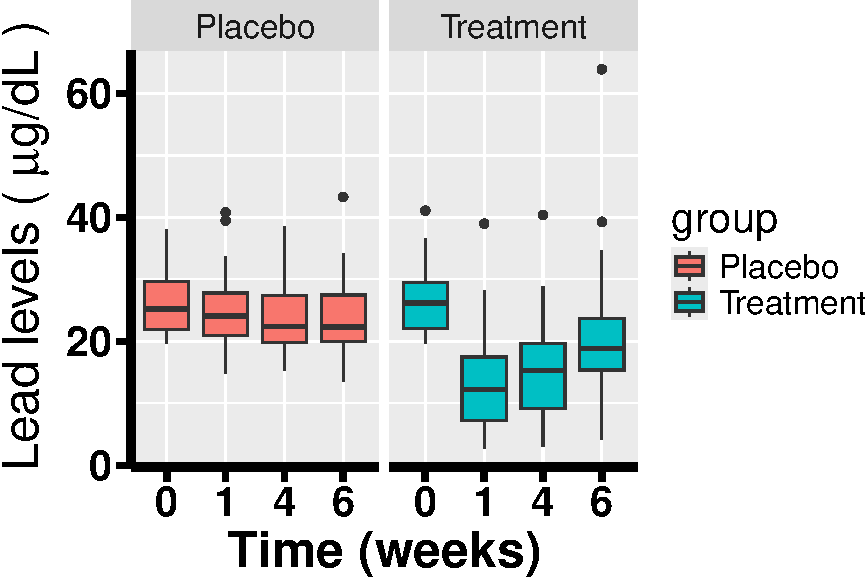
\includegraphics{Longi_EDA_files/figure-pdf/unnamed-chunk-10-1.pdf}

}

\end{figure}

\hypertarget{correlation-plot}{%
\subsection{Correlation Plot}\label{correlation-plot}}

Next, we can create a correlation plot using \texttt{GGally} package.

\begin{Shaded}
\begin{Highlighting}[]
\FunctionTok{ggpairs}\NormalTok{(TLC, }\AttributeTok{columns =} \FunctionTok{c}\NormalTok{(}\DecValTok{2}\SpecialCharTok{:}\DecValTok{5}\NormalTok{))}
\end{Highlighting}
\end{Shaded}

\begin{figure}[H]

{\centering 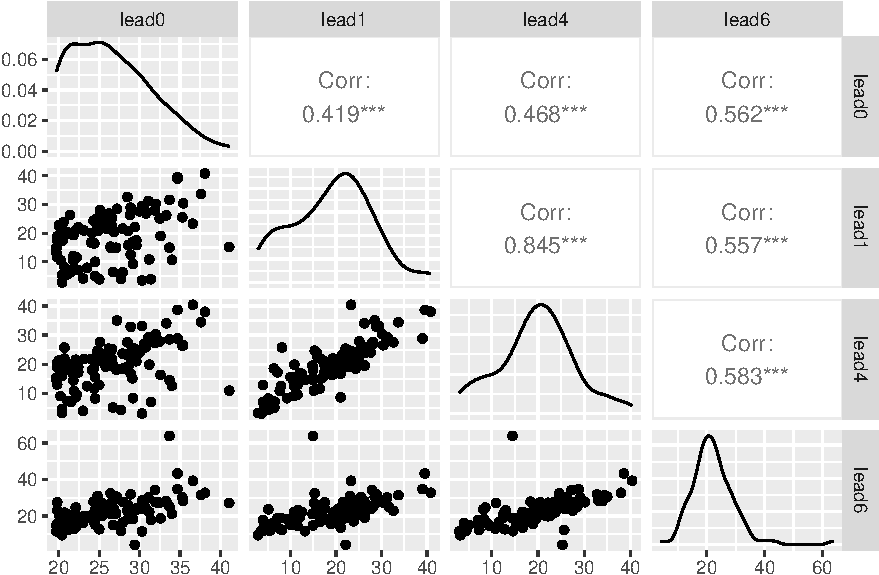
\includegraphics{Longi_EDA_files/figure-pdf/unnamed-chunk-11-1.pdf}

}

\end{figure}

\hypertarget{descriptive-statistics-for-longitudinal-data}{%
\section{Descriptive statistics for longitudinal
data}\label{descriptive-statistics-for-longitudinal-data}}

In this section we will calculate some summary statistics for our
continuous covariates. For simplicity I will be using the wide format of
the data since every observation (i.e.~row) will correspond to a unique
id. There are many functions in R which will calculate any type of
summary statistics you can think of. The most general is the summary()
function in base R which calculates the minimum, 1st Quartile (25\%
Percentile), Median, Mean, 3rd Quartile (75\%) and Maximum.

\hypertarget{calculate-summary-statistics-by-group}{%
\subsection{Calculate summary statistics by
group}\label{calculate-summary-statistics-by-group}}

\begin{Shaded}
\begin{Highlighting}[]
\CommentTok{\# Use by() function (in base R) to calculate summary statistics by Group}
\FunctionTok{by}\NormalTok{(TLC[, }\FunctionTok{c}\NormalTok{(}\StringTok{"lead0"}\NormalTok{, }\StringTok{"lead1"}\NormalTok{, }\StringTok{"lead4"}\NormalTok{, }\StringTok{"lead6"}\NormalTok{)], TLC[, }\StringTok{"group"}\NormalTok{], }\AttributeTok{FUN =}\NormalTok{ summary)}
\end{Highlighting}
\end{Shaded}

\begin{verbatim}
TLC[, "group"]: Placebo
     lead0           lead1           lead4           lead6      
 Min.   :19.70   Min.   :14.90   Min.   :15.30   Min.   :13.50  
 1st Qu.:21.88   1st Qu.:20.93   1st Qu.:19.82   1st Qu.:19.95  
 Median :25.25   Median :24.10   Median :22.45   Median :22.35  
 Mean   :26.27   Mean   :24.66   Mean   :24.07   Mean   :23.65  
 3rd Qu.:29.73   3rd Qu.:27.82   3rd Qu.:27.45   3rd Qu.:27.50  
 Max.   :38.10   Max.   :40.80   Max.   :38.60   Max.   :43.30  
------------------------------------------------------------ 
TLC[, "group"]: Treatment
     lead0           lead1            lead4            lead6      
 Min.   :19.70   Min.   : 2.800   Min.   : 3.000   Min.   : 4.10  
 1st Qu.:22.12   1st Qu.: 7.225   1st Qu.: 9.125   1st Qu.:15.40  
 Median :26.20   Median :12.250   Median :15.350   Median :18.85  
 Mean   :26.54   Mean   :13.522   Mean   :15.514   Mean   :20.76  
 3rd Qu.:29.55   3rd Qu.:17.500   3rd Qu.:19.725   3rd Qu.:23.75  
 Max.   :41.10   Max.   :39.000   Max.   :40.400   Max.   :63.90  
\end{verbatim}

\hypertarget{calculate-summary-statistics-for-all-bll-data-not-as-groups}{%
\subsection{Calculate summary statistics for all BLL data (not as
groups)}\label{calculate-summary-statistics-for-all-bll-data-not-as-groups}}

\begin{Shaded}
\begin{Highlighting}[]
\NormalTok{lead\_all }\OtherTok{\textless{}{-}} \FunctionTok{c}\NormalTok{(TLC}\SpecialCharTok{$}\NormalTok{lead0, TLC}\SpecialCharTok{$}\NormalTok{lead1, TLC}\SpecialCharTok{$}\NormalTok{lead4, TLC}\SpecialCharTok{$}\NormalTok{lead6)}
\FunctionTok{summary}\NormalTok{(lead\_all)  }\CommentTok{\#print summary statistics}
\end{Highlighting}
\end{Shaded}

\begin{verbatim}
   Min. 1st Qu.  Median    Mean 3rd Qu.    Max. 
   2.80   17.50   21.90   21.87   26.73   63.90 
\end{verbatim}

If you're in need of even more summary statistics you can use the
stat.desc package from the pastecs library.stat.desc provides you with
the additional following descriptive statistics: the number of values
(nbr.val), the number of null values (nbr.null), the number of missing
values (nbr.na), the minimal value (min), the maximal value (max), the
range (range, that is, max-min) and the sum of all non-missing values
(sum), the median (median), the mean (mean), the standard error on the
mean (SE.mean), the confidence interval of the mean (CI.mean) at the p
level, the variance (var), the standard deviation (std.dev) and the
variation coefficient (coef.var) defined as the standard deviation
divided by the mean.

\begin{Shaded}
\begin{Highlighting}[]
\DocumentationTok{\#\#\# Calculate summary statistics by group}
\FunctionTok{library}\NormalTok{(pastecs)}
\CommentTok{\# Use by() function (in base R) to calculate summary statistics by Group}
\FunctionTok{by}\NormalTok{(TLC[, }\FunctionTok{c}\NormalTok{(}\StringTok{"lead0"}\NormalTok{, }\StringTok{"lead1"}\NormalTok{, }\StringTok{"lead4"}\NormalTok{, }\StringTok{"lead6"}\NormalTok{)], TLC[, }\StringTok{"group"}\NormalTok{], }\AttributeTok{FUN =}\NormalTok{ stat.desc)}
\end{Highlighting}
\end{Shaded}

\begin{verbatim}
TLC[, "group"]: Placebo
                    lead0        lead1        lead4        lead6
nbr.val        50.0000000   50.0000000   50.0000000   50.0000000
nbr.null        0.0000000    0.0000000    0.0000000    0.0000000
nbr.na          0.0000000    0.0000000    0.0000000    0.0000000
min            19.7000010   14.9000000   15.3000000   13.5000000
max            38.0999980   40.7999990   38.5999980   43.2999990
range          18.3999970   25.8999990   23.2999980   29.7999990
sum          1313.5999970 1232.9999970 1203.5000030 1182.2999980
median         25.2500000   24.0999995   22.4500010   22.3500005
mean           26.2719999   24.6599999   24.0700001   23.6460000
SE.mean         0.7105160    0.7723275    0.8136150    0.7975893
CI.mean.0.95    1.4278353    1.5520502    1.6350205    1.6028157
var            25.2416481   29.8244892   33.0984669   31.8074323
std.dev         5.0241067    5.4611802    5.7531267    5.6398078
coef.var        0.1912343    0.2214591    0.2390165    0.2385100
------------------------------------------------------------ 
TLC[, "group"]: Treatment
                    lead0       lead1       lead4        lead6
nbr.val        50.0000000  50.0000000  50.0000000   50.0000000
nbr.null        0.0000000   0.0000000   0.0000000    0.0000000
nbr.na          0.0000000   0.0000000   0.0000000    0.0000000
min            19.7000010   2.8000000   3.0000000    4.0999999
max            41.0999980  39.0000000  40.4000020   63.9000020
range          21.3999970  36.2000000  37.4000020   59.8000021
sum          1326.9999960 676.0999983 775.6999992 1038.1000055
median         26.2000000  12.2500000  15.3500000   18.8499995
mean           26.5399999  13.5220000  15.5140000   20.7620001
SE.mean         0.7100675   1.0850535   1.1104697    1.3076288
CI.mean.0.95    1.4269341   2.1804967   2.2315724    2.6277784
var            25.2097935  58.8670567  61.6571480   85.4946530
std.dev         5.0209355   7.6724870   7.8522066    9.2463319
coef.var        0.1891837   0.5674077   0.5061368    0.4453488
\end{verbatim}

What do you observe in the variance-covariance matrices below? What
happens when the units change? Write 1-3 sentences.

\begin{Shaded}
\begin{Highlighting}[]
\DocumentationTok{\#\#\# Covariance Matrix for lead levels in ug/dL}
\FunctionTok{round}\NormalTok{(}\FunctionTok{cov}\NormalTok{(TLC[, }\FunctionTok{c}\NormalTok{(}\StringTok{"lead0"}\NormalTok{, }\StringTok{"lead1"}\NormalTok{, }\StringTok{"lead4"}\NormalTok{, }\StringTok{"lead6"}\NormalTok{)]), }\DecValTok{5}\NormalTok{)}
\end{Highlighting}
\end{Shaded}

\begin{verbatim}
         lead0    lead1    lead4    lead6
lead0 24.98905 18.16066 18.92146 21.78220
lead1 18.16066 75.22487 59.24104 37.48690
lead4 18.92146 59.24104 65.38539 36.54235
lead6 21.78220 37.48690 36.54235 60.15898
\end{verbatim}

\begin{Shaded}
\begin{Highlighting}[]
\DocumentationTok{\#\#\# Correlation Matrix for lead levels in mg/dL}
\FunctionTok{round}\NormalTok{(}\FunctionTok{cov}\NormalTok{(TLC[, }\FunctionTok{c}\NormalTok{(}\StringTok{"lead0"}\NormalTok{, }\StringTok{"lead1"}\NormalTok{, }\StringTok{"lead4"}\NormalTok{, }\StringTok{"lead6"}\NormalTok{)] }\SpecialCharTok{*} \DecValTok{10}\SpecialCharTok{\^{}{-}}\DecValTok{3}\NormalTok{), }\DecValTok{6}\NormalTok{)}
\end{Highlighting}
\end{Shaded}

\begin{verbatim}
        lead0   lead1   lead4   lead6
lead0 2.5e-05 1.8e-05 1.9e-05 2.2e-05
lead1 1.8e-05 7.5e-05 5.9e-05 3.7e-05
lead4 1.9e-05 5.9e-05 6.5e-05 3.7e-05
lead6 2.2e-05 3.7e-05 3.7e-05 6.0e-05
\end{verbatim}

What do you observe in the correlation matrices below? Write 1-3
sentences.

\begin{Shaded}
\begin{Highlighting}[]
\DocumentationTok{\#\#\# Correlation Matrix for lead levels in ug/dL}
\FunctionTok{round}\NormalTok{(}\FunctionTok{cor}\NormalTok{(TLC[, }\FunctionTok{c}\NormalTok{(}\StringTok{"lead0"}\NormalTok{, }\StringTok{"lead1"}\NormalTok{, }\StringTok{"lead4"}\NormalTok{, }\StringTok{"lead6"}\NormalTok{)]), }\DecValTok{3}\NormalTok{)}
\end{Highlighting}
\end{Shaded}

\begin{verbatim}
      lead0 lead1 lead4 lead6
lead0 1.000 0.419 0.468 0.562
lead1 0.419 1.000 0.845 0.557
lead4 0.468 0.845 1.000 0.583
lead6 0.562 0.557 0.583 1.000
\end{verbatim}

\begin{Shaded}
\begin{Highlighting}[]
\DocumentationTok{\#\#\# Correlation Matrix for lead levels in mg/dL}
\FunctionTok{round}\NormalTok{(}\FunctionTok{cor}\NormalTok{(TLC[, }\FunctionTok{c}\NormalTok{(}\StringTok{"lead0"}\NormalTok{, }\StringTok{"lead1"}\NormalTok{, }\StringTok{"lead4"}\NormalTok{, }\StringTok{"lead6"}\NormalTok{)] }\SpecialCharTok{*} \DecValTok{10}\SpecialCharTok{\^{}{-}}\DecValTok{3}\NormalTok{), }\DecValTok{3}\NormalTok{)}
\end{Highlighting}
\end{Shaded}

\begin{verbatim}
      lead0 lead1 lead4 lead6
lead0 1.000 0.419 0.468 0.562
lead1 0.419 1.000 0.845 0.557
lead4 0.468 0.845 1.000 0.583
lead6 0.562 0.557 0.583 1.000
\end{verbatim}

\hypertarget{sec-longi-GEE}{%
\chapter{Marginal Model (GEE)}\label{sec-longi-GEE}}

\hypertarget{introduction}{%
\section{Introduction}\label{introduction}}

For this section we will return to the TLC dataset with N = 100
participants in order to better understand marginal models for
longitudinal data when the outcome is continuous.

\hypertarget{required-packages}{%
\section{Required Packages}\label{required-packages}}

We will use the following packages:

\begin{itemize}
\item
  \texttt{nlme}: This package is for fitting and comparing Gaussian
  linear and nonlinear mixed-effects models. The variance-covariance
  structures for the residuals can be specified, and it is useful for
  data with repeated measures or longitudinal designs. We will use the
  \texttt{gls()} function to fit a linear model using generalized least
  squares.
\item
  \texttt{lme4}: This package is for fitting mixed-effects models. We
  will use the \texttt{lmer()} function to fit a linear model.
\end{itemize}

These packages are for applying the generalized estimating equations
(GEE) approach for fitting marginal generalized linear models to data
with repeated measures or longitudinal designs:

\begin{itemize}
\item
  \texttt{gee}: This is the ``Generalized Estimation Equation Solver''
  package.
\item
  \texttt{gpack}: This is the ``Generalized Estimating Equation
  Package'' package.
\item
  \texttt{geeM}: This is the ``Solve Generalized Estimating Equations''
  package.
\end{itemize}

\begin{Shaded}
\begin{Highlighting}[]
\FunctionTok{library}\NormalTok{(tidyr)  }\CommentTok{\#Allows for us to manipulate the data structure}
\FunctionTok{library}\NormalTok{(data.table)  }\CommentTok{\#Allows for us to manipulate the data structure}
\FunctionTok{library}\NormalTok{(ggplot2)  }\CommentTok{\#this makes better looking plots in R}

\CommentTok{\# new packages for models}
\FunctionTok{library}\NormalTok{(nlme)  }\CommentTok{\#used for the gls() function}
\FunctionTok{library}\NormalTok{(gee)  }\CommentTok{\# install.packages(\textquotesingle{}gee\textquotesingle{}), used for the gee() function}
\FunctionTok{library}\NormalTok{(geepack)  }\CommentTok{\# install.packages(\textquotesingle{}geepack\textquotesingle{}), used for the geeglm() function}
\FunctionTok{library}\NormalTok{(geeM)  }\CommentTok{\# install.packages(\textquotesingle{}geeM\textquotesingle{}), used for the geeglm() function}
\FunctionTok{theme\_set}\NormalTok{(}\FunctionTok{theme\_minimal}\NormalTok{())}
\end{Highlighting}
\end{Shaded}

\hypertarget{constructing-marginal-models}{%
\section{Constructing Marginal
Models}\label{constructing-marginal-models}}

Consider a continuous outcome \(Y\) which indicates a patient's blood
lead level (in micrograms per deciLiter \(\mu\)g/dL). The correct way to
write Y when doing a model like this would be as \(Y_{ij}\). \(Y_{ij}\)
is the lead blood level of patient i at time point j. Likewise the
covariates \(X = (1,X^1, \dots,X^p)\) would be as
\(X_{ij} = (1,X^1_{ij},\dots X^p_{ij})\), the p covariates for
individual i measured at time point j. 1 is simply the intercept. The
superscript here just represents the \(k-th\) covariate in the analysis
(i.e.~in other words we have p covariates).

In these different modelling strategies we always specify a link between
the mean of our distribution and the data,
\(E(y_{ij} \mid X_{ij}) = \mu_{ij} = g^{-1}(X^T_{ij}\beta)\). Here
\(g^{-1}\) is what is commonly referred to as a link function. It is
exactly what it sounds like. A function which links the mean of your
distribution to your data. There are many common link functions that
you've probably already dealt with in other regression courses. For
example there is the logit link function
\(g(\mu) =log(\frac{\mu}{1-\mu}) = X^T\beta\) that one uses when doing
logistic function.

When one is doing linear regression a common link function is just the
identity link \(g(\mu) =\mu = X^T\beta\).

\textbf{Here we introduce a few functions and corresponding packages to
fit these models:}

\textbf{1. Using the gls() function to fit a linear model using
generalized least squares}

The syntax for the function \texttt{gls()} in \texttt{nlme} package is

gls(model, data, correlation, weights, subset, method, na.action,
control, verbose)

\begin{itemize}
\tightlist
\item
  Description

  \begin{itemize}
  \tightlist
  \item
    \texttt{model}: A two-sided linear formula object describing the
    model
  \item
    \texttt{data}: Optional dataframe
  \item
    \texttt{correlation}: See description for details.

    \begin{itemize}
    \tightlist
    \item
      The corStruct object describes the within-group correlation
      structure.
    \item
      Note we use \texttt{corCompSymm} which has the following syntax:
      corCompSymm(value, form, fixed) compound symmetry structure
      corresponding to a constant correlation.
    \end{itemize}
  \item
    \texttt{weights}: See description for details.

    \begin{itemize}
    \tightlist
    \item
      Describes the variance function.
    \item
      Note we use \texttt{varClasses} which defines standard classes of
      variance function structures and use \texttt{varIdent} which
      describes constant variance(s), that is generally used to allow
      different variances.
    \end{itemize}
  \end{itemize}
\end{itemize}

We consider the first model discussed in lecture. This model includes
time as a categorical covariate and also includes an interaction term to
account and adjust for any possible discrepancies between the treatment
and control.

Model 1:
\[E(y_{ij} \mid X_{ij}) = \beta_0 +  \beta_{trt}trt +  \beta_{T_1}T_1 +  \beta_{T_4}T_4 +  \beta_{T_6}T_6 +  \]
\[\beta_{trt:T_1}trt*T_1+ \beta_{trt:T_4}trt*T_4 + \beta_{trt:T_6}trt*T_6\]

\begin{Shaded}
\begin{Highlighting}[]
\CommentTok{\# Model fit with compound symmetry heterogeneous variances}

\CommentTok{\# Model 1: Response Profiles (time T categorical)}
\NormalTok{fit.compsym }\OtherTok{\textless{}{-}} \FunctionTok{gls}\NormalTok{(measurements }\SpecialCharTok{\textasciitilde{}} \FunctionTok{factor}\NormalTok{(group) }\SpecialCharTok{*} \FunctionTok{factor}\NormalTok{(level), }\AttributeTok{data =}\NormalTok{ long\_TLC,}
    \AttributeTok{corr =} \FunctionTok{corCompSymm}\NormalTok{(, }\AttributeTok{form =} \SpecialCharTok{\textasciitilde{}}\FunctionTok{factor}\NormalTok{(level) }\SpecialCharTok{|}\NormalTok{ id), }\AttributeTok{weights =} \FunctionTok{varIdent}\NormalTok{(}\AttributeTok{form =} \SpecialCharTok{\textasciitilde{}}\DecValTok{1} \SpecialCharTok{|}
        \FunctionTok{factor}\NormalTok{(level)))}
\FunctionTok{summary}\NormalTok{(fit.compsym)}
\end{Highlighting}
\end{Shaded}

\begin{verbatim}
Generalized least squares fit by REML
  Model: measurements ~ factor(group) * factor(level) 
  Data: long_TLC 
      AIC      BIC   logLik
  2459.96 2511.587 -1216.98

Correlation Structure: Compound symmetry
 Formula: ~factor(level) | id 
 Parameter estimate(s):
      Rho 
0.6102708 
Variance function:
 Structure: Different standard deviations per stratum
 Formula: ~1 | factor(level) 
 Parameter estimates:
   lead0    lead1    lead4    lead6 
1.000000 1.279672 1.323197 1.519220 

Coefficients:
                                            Value Std.Error   t-value p-value
(Intercept)                                26.272 0.7237951  36.29757  0.0000
factor(group)Treatment                      0.268 1.0236008   0.26182  0.7936
factor(level)lead1                         -1.612 0.7506796  -2.14739  0.0324
factor(level)lead4                         -2.202 0.7713883  -2.85459  0.0045
factor(level)lead6                         -2.626 0.8726932  -3.00908  0.0028
factor(group)Treatment:factor(level)lead1 -11.406 1.0616213 -10.74394  0.0000
factor(group)Treatment:factor(level)lead4  -8.824 1.0909078  -8.08868  0.0000
factor(group)Treatment:factor(level)lead6  -3.152 1.2341746  -2.55393  0.0110

 Correlation: 
                                          (Intr) fct()T fct()1 fct()4 fct()6
factor(group)Treatment                    -0.707                            
factor(level)lead1                        -0.211  0.149                     
factor(level)lead4                        -0.181  0.128  0.402              
factor(level)lead6                        -0.060  0.043  0.383  0.383       
factor(group)Treatment:factor(level)lead1  0.149 -0.211 -0.707 -0.285 -0.270
factor(group)Treatment:factor(level)lead4  0.128 -0.181 -0.285 -0.707 -0.271
factor(group)Treatment:factor(level)lead6  0.043 -0.060 -0.270 -0.271 -0.707
                                          f()T:()1 f()T:()4
factor(group)Treatment                                     
factor(level)lead1                                         
factor(level)lead4                                         
factor(level)lead6                                         
factor(group)Treatment:factor(level)lead1                  
factor(group)Treatment:factor(level)lead4  0.402           
factor(group)Treatment:factor(level)lead6  0.383    0.383  

Standardized residuals:
       Min         Q1        Med         Q3        Max 
-2.1429199 -0.6927789 -0.1528885  0.5263121  5.5480303 

Residual standard error: 5.118004 
Degrees of freedom: 400 total; 392 residual
\end{verbatim}

\begin{Shaded}
\begin{Highlighting}[]
\FunctionTok{anova}\NormalTok{(fit.compsym)}
\end{Highlighting}
\end{Shaded}

\begin{verbatim}
Denom. DF: 392 
                            numDF   F-value p-value
(Intercept)                     1 2438.1366  <.0001
factor(group)                   1    7.1161   0.008
factor(level)                   3   80.5490  <.0001
factor(group):factor(level)     3   46.9288  <.0001
\end{verbatim}

\textbf{2. Next, we discuss Marginal Models (GEE) and three R Packages }

\textbf{1. Using the \texttt{gee} package}

The syntax for the function \texttt{gee()} in \texttt{gee} package is

gee(formula, id, data, family = gaussian, constr = `independence',Mv)

\begin{itemize}
\tightlist
\item
  Using the \texttt{GEE} Package

  \begin{itemize}
  \tightlist
  \item
    \texttt{formula}: Symbolic description of the model to be fitted
  \item
    \texttt{family}: Description of the error distribution and link
    function
  \item
    \texttt{data}: Optional dataframe
  \item
    \texttt{id}: Vector that identifies the clusters
  \item
    \texttt{constr}: Working correlation structure: ``independence'',
    ``exchangeable'', ``AR-M'', ``unstructured''
  \item
    \texttt{Mv}: order of AR correlation (AR1: Mv = 1)
  \end{itemize}
\end{itemize}

Consider the same model 1 defined earlier:

\begin{Shaded}
\begin{Highlighting}[]
\CommentTok{\# Model 1: Response Profiles (time T categorical)}
\NormalTok{mod\_tlc\_gee }\OtherTok{\textless{}{-}} \FunctionTok{gee}\NormalTok{(measurements }\SpecialCharTok{\textasciitilde{}}\NormalTok{ level }\SpecialCharTok{+}\NormalTok{ group }\SpecialCharTok{+}\NormalTok{ level }\SpecialCharTok{*}\NormalTok{ group, }\AttributeTok{id =}\NormalTok{ id, }\AttributeTok{data =}\NormalTok{ long\_TLC,}
    \AttributeTok{family =} \FunctionTok{gaussian}\NormalTok{(}\AttributeTok{link =} \StringTok{"identity"}\NormalTok{), }\AttributeTok{corstr =} \StringTok{"unstructured"}\NormalTok{)}
\end{Highlighting}
\end{Shaded}

\begin{verbatim}
              (Intercept)                levellead1                levellead4 
                   26.272                    -1.612                    -2.202 
               levellead6            groupTreatment levellead1:groupTreatment 
                   -2.626                     0.268                   -11.406 
levellead4:groupTreatment levellead6:groupTreatment 
                   -8.824                    -3.152 
\end{verbatim}

\begin{Shaded}
\begin{Highlighting}[]
\FunctionTok{summary}\NormalTok{(mod\_tlc\_gee)}
\end{Highlighting}
\end{Shaded}

\begin{verbatim}

 GEE:  GENERALIZED LINEAR MODELS FOR DEPENDENT DATA
 gee S-function, version 4.13 modified 98/01/27 (1998) 

Model:
 Link:                      Identity 
 Variance to Mean Relation: Gaussian 
 Correlation Structure:     Unstructured 

Call:
gee(formula = measurements ~ level + group + level * group, id = id, 
    data = long_TLC, family = gaussian(link = "identity"), corstr = "unstructured")

Summary of Residuals:
        Min          1Q      Median          3Q         Max 
-16.6620002  -4.6205000  -0.9930005   3.6724993  43.1380019 


Coefficients:
                          Estimate Naive S.E.    Naive z Robust S.E.
(Intercept)                 26.272  0.9370175 28.0378980   0.7033749
levellead1                  -1.612  0.9958441 -1.6187272   0.4330324
levellead4                  -2.202  0.9838821 -2.2380730   0.4386752
levellead6                  -2.626  0.9316319 -2.8187098   0.5278091
groupTreatment               0.268  1.3251428  0.2022423   0.9944085
levellead1:groupTreatment  -11.406  1.4083363 -8.0989180   1.1086833
levellead4:groupTreatment   -8.824  1.3914194 -6.3417258   1.1408849
levellead6:groupTreatment   -3.152  1.3175265 -2.3923617   1.2439296
                             Robust z
(Intercept)                37.3513450
levellead1                 -3.7225849
levellead4                 -5.0196593
levellead6                 -4.9752836
groupTreatment              0.2695069
levellead1:groupTreatment -10.2878795
levellead4:groupTreatment  -7.7343471
levellead6:groupTreatment  -2.5339053

Estimated Scale Parameter:  43.90009
Number of Iterations:  1

Working Correlation
          [,1]      [,2]      [,3]      [,4]
[1,] 1.0000000 0.4352485 0.4487346 0.5057310
[2,] 0.4352485 1.0000000 0.8094551 0.6759677
[3,] 0.4487346 0.8094551 1.0000000 0.6975035
[4,] 0.5057310 0.6759677 0.6975035 1.0000000
\end{verbatim}

\textbf{2. Using the \texttt{geepack} package}

The syntax for the function \texttt{geeglm()} in \texttt{geepack}
package is

geeglm(formula, family = gaussian, data, id, zcor = NULL, constr,
std.err = `san.se')

\begin{itemize}
\tightlist
\item
  Using the \texttt{geepack} package

  \begin{itemize}
  \tightlist
  \item
    \texttt{formula}: Symbolic description of the model to be fitted
  \item
    \texttt{family}: Description of the error distribution and link
    function
  \item
    \texttt{data}: Optional dataframe
  \item
    \texttt{id}: Vector that identifies the clusters
  \item
    \texttt{contr}: A character string specifying the correlation
    structure. The following are permitted: ``independence'',
    ``exchangeable'', ``ar1'', ``unstructured'' and ``userdefined''
  \item
    \texttt{zcor}: Enter a user defined correlation structure
  \end{itemize}
\end{itemize}

Consider the same model 1 defined earlier

\begin{Shaded}
\begin{Highlighting}[]
\CommentTok{\# Model 1: Response Profiles (time T categorical)}
\NormalTok{mod\_tlc\_geep }\OtherTok{\textless{}{-}} \FunctionTok{geeglm}\NormalTok{(measurements }\SpecialCharTok{\textasciitilde{}}\NormalTok{ level }\SpecialCharTok{+}\NormalTok{ group }\SpecialCharTok{+}\NormalTok{ level }\SpecialCharTok{*}\NormalTok{ group, }\AttributeTok{id =}\NormalTok{ id, }\AttributeTok{data =}\NormalTok{ long\_TLC,}
    \AttributeTok{family =} \FunctionTok{gaussian}\NormalTok{(}\AttributeTok{link =} \StringTok{"identity"}\NormalTok{), }\AttributeTok{corstr =} \StringTok{"unstructured"}\NormalTok{)}

\FunctionTok{summary}\NormalTok{(mod\_tlc\_geep)}
\end{Highlighting}
\end{Shaded}

\begin{verbatim}

Call:
geeglm(formula = measurements ~ level + group + level * group, 
    family = gaussian(link = "identity"), data = long_TLC, id = id, 
    corstr = "unstructured")

 Coefficients:
                          Estimate  Std.err     Wald Pr(>|W|)    
(Intercept)                26.2720   0.7034 1395.123  < 2e-16 ***
levellead1                 -1.6120   0.4330   13.858 0.000197 ***
levellead4                 -2.2020   0.4387   25.197 5.18e-07 ***
levellead6                 -2.6260   0.5278   24.753 6.52e-07 ***
groupTreatment              0.2680   0.9944    0.073 0.787540    
levellead1:groupTreatment -11.4060   1.1087  105.840  < 2e-16 ***
levellead4:groupTreatment  -8.8240   1.1409   59.820 1.04e-14 ***
levellead6:groupTreatment  -3.1520   1.2439    6.421 0.011280 *  
---
Signif. codes:  0 '***' 0.001 '**' 0.01 '*' 0.05 '.' 0.1 ' ' 1

Correlation structure = unstructured 
Estimated Scale Parameters:

            Estimate Std.err
(Intercept)    43.02   6.583
  Link = identity 

Estimated Correlation Parameters:
          Estimate Std.err
alpha.1:2   0.4352 0.07616
alpha.1:3   0.4487 0.08482
alpha.1:4   0.5057 0.05768
alpha.2:3   0.8095 0.11232
alpha.2:4   0.6760 0.10359
alpha.3:4   0.6975 0.13711
Number of clusters:   100  Maximum cluster size: 4 
\end{verbatim}

We can use the QIC() function from the geepack package.

\begin{Shaded}
\begin{Highlighting}[]
\FunctionTok{QIC}\NormalTok{(mod\_tlc\_geep)}
\end{Highlighting}
\end{Shaded}

\begin{verbatim}
      QIC      QICu Quasi Lik       CIC    params      QICC 
    17225     17225     -8604         8         8     17230 
\end{verbatim}

\textbf{3. Using the geeM package}

The syntax for the function \texttt{geem()} in \texttt{geeM} package is

geem(formula, id, waves = NULL, data, family = gaussian, constr =
``independence'', Mv = 1)

\begin{itemize}
\tightlist
\item
  Using the \texttt{geeM} package

  \begin{itemize}
  \tightlist
  \item
    \texttt{formula}: Symbolic description of the model to be fitted
  \item
    \texttt{id}: Vector that identifies the clusters
  \item
    \texttt{data}: Optional dataframe
  \item
    \texttt{family}: Description of the error distribution and link
    function
  \item
    \texttt{constr}: A character string specifying the correlation
    structure. Allowed structures are: ``independence'',
    ``exchangeable'' (equal correlation), ``ar1'' (exponential decay),
    ``m-dependent'' (m-diagonal), ``unstructured'', ``fixed'', and
    ``userdefined''.
  \item
    \texttt{Mv}: for ``m-dependent'', the value for m.
  \end{itemize}
\end{itemize}

Consider the same model 1 defined earlier

\begin{Shaded}
\begin{Highlighting}[]
\CommentTok{\# Model 1: Response Profiles (time T categorical)}
\NormalTok{mod\_tlc\_geeM }\OtherTok{\textless{}{-}} \FunctionTok{geem}\NormalTok{(measurements }\SpecialCharTok{\textasciitilde{}}\NormalTok{ level }\SpecialCharTok{+}\NormalTok{ group }\SpecialCharTok{+}\NormalTok{ level }\SpecialCharTok{*}\NormalTok{ group, }\AttributeTok{id =}\NormalTok{ id, }\AttributeTok{data =}\NormalTok{ long\_TLC,}
    \AttributeTok{family =} \FunctionTok{gaussian}\NormalTok{(}\AttributeTok{link =} \StringTok{"identity"}\NormalTok{), }\AttributeTok{corstr =} \StringTok{"unstructured"}\NormalTok{)}

\FunctionTok{summary}\NormalTok{(mod\_tlc\_geeM)}
\end{Highlighting}
\end{Shaded}

\begin{verbatim}
                          Estimates Model SE Robust SE     wald         p
(Intercept)                  26.270    1.143    0.7034  37.3500 0.000e+00
levellead1                   -1.612    1.543    0.4330  -3.7230 1.972e-04
levellead4                   -2.202    1.487    0.4387  -5.0200 5.200e-07
levellead6                   -2.626    1.270    0.5278  -4.9750 6.500e-07
groupTreatment                0.268    1.617    0.9944   0.2695 7.875e-01
levellead1:groupTreatment   -11.410    2.182    1.1090 -10.2900 0.000e+00
levellead4:groupTreatment    -8.824    2.103    1.1410  -7.7340 0.000e+00
levellead6:groupTreatment    -3.152    1.795    1.2440  -2.5340 1.128e-02

 Working Correlation: 
       [,1]   [,2]   [,3]   [,4]
[1,] 1.0000 0.0893 0.1546 0.3835
[2,] 0.0893 1.0000 1.0716 0.6018
[3,] 0.1546 1.0716 1.0000 0.5901
[4,] 0.3835 0.6018 0.5901 1.0000
 Correlation Structure:  unstructured 
 Est. Scale Parameter:  65.36 

 Number of GEE iterations: 1 
 Number of Clusters:  100    Maximum Cluster Size:  4 
 Number of observations with nonzero weight:  400 
\end{verbatim}

\hypertarget{response-profile-analysis}{%
\section{Response Profile Analysis}\label{response-profile-analysis}}

Model 1:
\[E(y_{ij} \mid X_{ij}) = \beta_0 +  \beta_{trt}trt +  \beta_{T_1}T_1 +  \beta_{T_4}T_4 +  \beta_{T_6}T_6 +  \]
\[\beta_{trt:T_1}trt*T_1+ \beta_{trt:T_4}trt*T_4 + \beta_{trt:T_6}trt*T_6\]

This model includes time as a categorical covariate and also includes an
interaction term to account and adjust for any possible discrepancies
between the treatment and control.

Using the GLS approach, we can fit a model to include time, treatment,
and their interaction as categorical variables (use dummy variables).
What is your overall conclusion?

\begin{Shaded}
\begin{Highlighting}[]
\CommentTok{\# Recall the example above from the nlme package}

\CommentTok{\# Model 1: Response Profiles (time T categorical)}
\NormalTok{resprof\_gls\_mod\_1 }\OtherTok{\textless{}{-}} \FunctionTok{gls}\NormalTok{(measurements }\SpecialCharTok{\textasciitilde{}} \FunctionTok{factor}\NormalTok{(group) }\SpecialCharTok{*} \FunctionTok{factor}\NormalTok{(level), }\AttributeTok{data =}\NormalTok{ long\_TLC,}
    \AttributeTok{corr =} \FunctionTok{corCompSymm}\NormalTok{(, }\AttributeTok{form =} \SpecialCharTok{\textasciitilde{}}\FunctionTok{factor}\NormalTok{(level) }\SpecialCharTok{|}\NormalTok{ id), }\AttributeTok{weights =} \FunctionTok{varIdent}\NormalTok{(}\AttributeTok{form =} \SpecialCharTok{\textasciitilde{}}\DecValTok{1} \SpecialCharTok{|}
        \FunctionTok{factor}\NormalTok{(level)))}

\CommentTok{\# Print summary}
\FunctionTok{summary}\NormalTok{(resprof\_gls\_mod\_1)}
\end{Highlighting}
\end{Shaded}

\begin{verbatim}
Generalized least squares fit by REML
  Model: measurements ~ factor(group) * factor(level) 
  Data: long_TLC 
   AIC  BIC logLik
  2460 2512  -1217

Correlation Structure: Compound symmetry
 Formula: ~factor(level) | id 
 Parameter estimate(s):
   Rho 
0.6103 
Variance function:
 Structure: Different standard deviations per stratum
 Formula: ~1 | factor(level) 
 Parameter estimates:
lead0 lead1 lead4 lead6 
1.000 1.280 1.323 1.519 

Coefficients:
                                            Value Std.Error t-value p-value
(Intercept)                                26.272    0.7238   36.30  0.0000
factor(group)Treatment                      0.268    1.0236    0.26  0.7936
factor(level)lead1                         -1.612    0.7507   -2.15  0.0324
factor(level)lead4                         -2.202    0.7714   -2.85  0.0045
factor(level)lead6                         -2.626    0.8727   -3.01  0.0028
factor(group)Treatment:factor(level)lead1 -11.406    1.0616  -10.74  0.0000
factor(group)Treatment:factor(level)lead4  -8.824    1.0909   -8.09  0.0000
factor(group)Treatment:factor(level)lead6  -3.152    1.2342   -2.55  0.0110

 Correlation: 
                                          (Intr) fct()T fct()1 fct()4 fct()6
factor(group)Treatment                    -0.707                            
factor(level)lead1                        -0.211  0.149                     
factor(level)lead4                        -0.181  0.128  0.402              
factor(level)lead6                        -0.060  0.043  0.383  0.383       
factor(group)Treatment:factor(level)lead1  0.149 -0.211 -0.707 -0.285 -0.270
factor(group)Treatment:factor(level)lead4  0.128 -0.181 -0.285 -0.707 -0.271
factor(group)Treatment:factor(level)lead6  0.043 -0.060 -0.270 -0.271 -0.707
                                          f()T:()1 f()T:()4
factor(group)Treatment                                     
factor(level)lead1                                         
factor(level)lead4                                         
factor(level)lead6                                         
factor(group)Treatment:factor(level)lead1                  
factor(group)Treatment:factor(level)lead4  0.402           
factor(group)Treatment:factor(level)lead6  0.383    0.383  

Standardized residuals:
    Min      Q1     Med      Q3     Max 
-2.1429 -0.6928 -0.1529  0.5263  5.5480 

Residual standard error: 5.118 
Degrees of freedom: 400 total; 392 residual
\end{verbatim}

Using the GEE approach, we can fit a model to include time, treatment,
and their interaction as categorical variables (use dummy variables).
Assume unstructured covariance model. Compare model estimates, standard
errors, and covariance matrices with those from the methods you used in
the previous question.

\begin{Shaded}
\begin{Highlighting}[]
\NormalTok{model\_1 }\OtherTok{\textless{}{-}} \FunctionTok{geeglm}\NormalTok{(measurements }\SpecialCharTok{\textasciitilde{}}\NormalTok{ group }\SpecialCharTok{+} \FunctionTok{as.factor}\NormalTok{(time) }\SpecialCharTok{+} \FunctionTok{as.factor}\NormalTok{(time) }\SpecialCharTok{*}\NormalTok{ group,}
    \AttributeTok{id =}\NormalTok{ id, }\AttributeTok{data =}\NormalTok{ long\_TLC, }\AttributeTok{family =} \FunctionTok{gaussian}\NormalTok{(}\AttributeTok{link =} \StringTok{"identity"}\NormalTok{), }\AttributeTok{corstr =} \StringTok{"unstructured"}\NormalTok{)}
\FunctionTok{summary}\NormalTok{(model\_1)}
\end{Highlighting}
\end{Shaded}

\begin{verbatim}

Call:
geeglm(formula = measurements ~ group + as.factor(time) + as.factor(time) * 
    group, family = gaussian(link = "identity"), data = long_TLC, 
    id = id, corstr = "unstructured")

 Coefficients:
                                Estimate Std.err    Wald Pr(>|W|)    
(Intercept)                       26.272   0.703 1395.12  < 2e-16 ***
groupTreatment                     0.268   0.994    0.07   0.7875    
as.factor(time)1                  -1.612   0.433   13.86   0.0002 ***
as.factor(time)4                  -2.202   0.439   25.20  5.2e-07 ***
as.factor(time)6                  -2.626   0.528   24.75  6.5e-07 ***
groupTreatment:as.factor(time)1  -11.406   1.109  105.84  < 2e-16 ***
groupTreatment:as.factor(time)4   -8.824   1.141   59.82  1.0e-14 ***
groupTreatment:as.factor(time)6   -3.152   1.244    6.42   0.0113 *  
---
Signif. codes:  0 '***' 0.001 '**' 0.01 '*' 0.05 '.' 0.1 ' ' 1

Correlation structure = unstructured 
Estimated Scale Parameters:

            Estimate Std.err
(Intercept)       43    6.58
  Link = identity 

Estimated Correlation Parameters:
          Estimate Std.err
alpha.1:2    0.435  0.0762
alpha.1:3    0.449  0.0848
alpha.1:4    0.506  0.0577
alpha.2:3    0.809  0.1123
alpha.2:4    0.676  0.1036
alpha.3:4    0.698  0.1371
Number of clusters:   100  Maximum cluster size: 4 
\end{verbatim}

\begin{Shaded}
\begin{Highlighting}[]
\CommentTok{\# Recall the example above from the geepack package}

\CommentTok{\# Model 1: Response Profiles (time T categorical)}
\NormalTok{resprof\_gee\_mod\_1 }\OtherTok{\textless{}{-}} \FunctionTok{geeglm}\NormalTok{(measurements }\SpecialCharTok{\textasciitilde{}}\NormalTok{ level }\SpecialCharTok{+}\NormalTok{ group }\SpecialCharTok{+}\NormalTok{ level }\SpecialCharTok{*}\NormalTok{ group, }\AttributeTok{id =}\NormalTok{ id,}
    \AttributeTok{data =}\NormalTok{ long\_TLC, }\AttributeTok{family =} \FunctionTok{gaussian}\NormalTok{(}\AttributeTok{link =} \StringTok{"identity"}\NormalTok{), }\AttributeTok{corstr =} \StringTok{"unstructured"}\NormalTok{)}

\CommentTok{\# Print summary}
\FunctionTok{summary}\NormalTok{(resprof\_gee\_mod\_1)}
\end{Highlighting}
\end{Shaded}

\begin{verbatim}

Call:
geeglm(formula = measurements ~ level + group + level * group, 
    family = gaussian(link = "identity"), data = long_TLC, id = id, 
    corstr = "unstructured")

 Coefficients:
                          Estimate Std.err    Wald Pr(>|W|)    
(Intercept)                 26.272   0.703 1395.12  < 2e-16 ***
levellead1                  -1.612   0.433   13.86   0.0002 ***
levellead4                  -2.202   0.439   25.20  5.2e-07 ***
levellead6                  -2.626   0.528   24.75  6.5e-07 ***
groupTreatment               0.268   0.994    0.07   0.7875    
levellead1:groupTreatment  -11.406   1.109  105.84  < 2e-16 ***
levellead4:groupTreatment   -8.824   1.141   59.82  1.0e-14 ***
levellead6:groupTreatment   -3.152   1.244    6.42   0.0113 *  
---
Signif. codes:  0 '***' 0.001 '**' 0.01 '*' 0.05 '.' 0.1 ' ' 1

Correlation structure = unstructured 
Estimated Scale Parameters:

            Estimate Std.err
(Intercept)       43    6.58
  Link = identity 

Estimated Correlation Parameters:
          Estimate Std.err
alpha.1:2    0.435  0.0762
alpha.1:3    0.449  0.0848
alpha.1:4    0.506  0.0577
alpha.2:3    0.809  0.1123
alpha.2:4    0.676  0.1036
alpha.3:4    0.698  0.1371
Number of clusters:   100  Maximum cluster size: 4 
\end{verbatim}

\begin{Shaded}
\begin{Highlighting}[]
\CommentTok{\# Print QIC}
\FunctionTok{QIC}\NormalTok{(resprof\_gee\_mod\_1)}
\end{Highlighting}
\end{Shaded}

\begin{verbatim}
      QIC      QICu Quasi Lik       CIC    params      QICC 
    17225     17225     -8604         8         8     17230 
\end{verbatim}

\hypertarget{parametric-curves}{%
\section{Parametric Curves}\label{parametric-curves}}

\begin{Shaded}
\begin{Highlighting}[]
\CommentTok{\# create new variable to make time continuous}
\NormalTok{long\_TLC}\SpecialCharTok{$}\NormalTok{week }\OtherTok{=} \DecValTok{0}  \CommentTok{\#baseline, week 0 }
\NormalTok{long\_TLC}\SpecialCharTok{$}\NormalTok{week[long\_TLC}\SpecialCharTok{$}\NormalTok{level }\SpecialCharTok{==} \StringTok{"lead1"}\NormalTok{] }\OtherTok{=} \DecValTok{1}  \CommentTok{\#week 1}
\NormalTok{long\_TLC}\SpecialCharTok{$}\NormalTok{week[long\_TLC}\SpecialCharTok{$}\NormalTok{level }\SpecialCharTok{==} \StringTok{"lead4"}\NormalTok{] }\OtherTok{=} \DecValTok{4}  \CommentTok{\#week 4}
\NormalTok{long\_TLC}\SpecialCharTok{$}\NormalTok{week[long\_TLC}\SpecialCharTok{$}\NormalTok{level }\SpecialCharTok{==} \StringTok{"lead6"}\NormalTok{] }\OtherTok{=} \DecValTok{6}  \CommentTok{\#week 6}
\end{Highlighting}
\end{Shaded}

\begin{Shaded}
\begin{Highlighting}[]
\NormalTok{parcurv\_mod\_2 }\OtherTok{\textless{}{-}} \FunctionTok{gls}\NormalTok{(measurements }\SpecialCharTok{\textasciitilde{}} \FunctionTok{factor}\NormalTok{(group) }\SpecialCharTok{+}\NormalTok{ week, }\AttributeTok{data =}\NormalTok{ long\_TLC, }\AttributeTok{corr =} \FunctionTok{corCompSymm}\NormalTok{(,}
    \AttributeTok{form =} \SpecialCharTok{\textasciitilde{}}\NormalTok{week }\SpecialCharTok{|}\NormalTok{ id), }\AttributeTok{weights =} \FunctionTok{varIdent}\NormalTok{(}\AttributeTok{form =} \SpecialCharTok{\textasciitilde{}}\DecValTok{1} \SpecialCharTok{|}\NormalTok{ week), }\AttributeTok{method =} \StringTok{"REML"}\NormalTok{)}

\CommentTok{\# Print summary}
\FunctionTok{summary}\NormalTok{(parcurv\_mod\_2)}
\end{Highlighting}
\end{Shaded}

\begin{verbatim}
Generalized least squares fit by REML
  Model: measurements ~ factor(group) + week 
  Data: long_TLC 
   AIC  BIC logLik
  2663 2695  -1323

Correlation Structure: Compound symmetry
 Formula: ~week | id 
 Parameter estimate(s):
  Rho 
0.659 
Variance function:
 Structure: Different standard deviations per stratum
 Formula: ~1 | week 
 Parameter estimates:
   0    1    4    6 
1.00 2.22 1.83 1.54 

Coefficients:
                       Value Std.Error t-value p-value
(Intercept)            26.53     0.742    35.8  0.0000
factor(group)Treatment  2.30     1.049     2.2  0.0291
week                   -0.58     0.098    -5.9  0.0000

 Correlation: 
                       (Intr) fct()T
factor(group)Treatment -0.707       
week                   -0.035  0.000

Standardized residuals:
    Min      Q1     Med      Q3     Max 
-2.5179 -1.0636 -0.3993  0.0715  4.5654 

Residual standard error: 5.48 
Degrees of freedom: 400 total; 397 residual
\end{verbatim}

\hypertarget{more-marginal-models}{%
\section{More Marginal Models}\label{more-marginal-models}}

\textbf{Model 1: time is categorical, main effects, interaction terms}

Model 1:
\[E(y_{ij} \mid X_{ij}) = \beta_0 +  \beta_{trt}trt +  \beta_{T_1}T_1 +  \beta_{T_4}T_4 +  \beta_{T_6}T_6 +  \beta_{trt:T_1}trt*T_1+ \]
\[\beta_{trt:T_4}trt*T_4 + \beta_{trt:T_6}trt*T_6\]

This model includes time as a categorical covariate and also includes an
interaction term to account and adjust for any possible discrepancies
between the treatment and control.

\begin{Shaded}
\begin{Highlighting}[]
\NormalTok{model\_1 }\OtherTok{\textless{}{-}} \FunctionTok{geeglm}\NormalTok{(measurements }\SpecialCharTok{\textasciitilde{}}\NormalTok{ group }\SpecialCharTok{+} \FunctionTok{as.factor}\NormalTok{(time) }\SpecialCharTok{+} \FunctionTok{as.factor}\NormalTok{(time) }\SpecialCharTok{*}\NormalTok{ group,}
    \AttributeTok{id =}\NormalTok{ id, }\AttributeTok{data =}\NormalTok{ long\_TLC, }\AttributeTok{family =} \FunctionTok{gaussian}\NormalTok{(}\AttributeTok{link =} \StringTok{"identity"}\NormalTok{), }\AttributeTok{corstr =} \StringTok{"unstructured"}\NormalTok{)}

\CommentTok{\# Print summary}
\FunctionTok{summary}\NormalTok{(model\_1)}
\end{Highlighting}
\end{Shaded}

\begin{verbatim}

Call:
geeglm(formula = measurements ~ group + as.factor(time) + as.factor(time) * 
    group, family = gaussian(link = "identity"), data = long_TLC, 
    id = id, corstr = "unstructured")

 Coefficients:
                                Estimate Std.err    Wald Pr(>|W|)    
(Intercept)                       26.272   0.703 1395.12  < 2e-16 ***
groupTreatment                     0.268   0.994    0.07   0.7875    
as.factor(time)1                  -1.612   0.433   13.86   0.0002 ***
as.factor(time)4                  -2.202   0.439   25.20  5.2e-07 ***
as.factor(time)6                  -2.626   0.528   24.75  6.5e-07 ***
groupTreatment:as.factor(time)1  -11.406   1.109  105.84  < 2e-16 ***
groupTreatment:as.factor(time)4   -8.824   1.141   59.82  1.0e-14 ***
groupTreatment:as.factor(time)6   -3.152   1.244    6.42   0.0113 *  
---
Signif. codes:  0 '***' 0.001 '**' 0.01 '*' 0.05 '.' 0.1 ' ' 1

Correlation structure = unstructured 
Estimated Scale Parameters:

            Estimate Std.err
(Intercept)       43    6.58
  Link = identity 

Estimated Correlation Parameters:
          Estimate Std.err
alpha.1:2    0.435  0.0762
alpha.1:3    0.449  0.0848
alpha.1:4    0.506  0.0577
alpha.2:3    0.809  0.1123
alpha.2:4    0.676  0.1036
alpha.3:4    0.698  0.1371
Number of clusters:   100  Maximum cluster size: 4 
\end{verbatim}

\textbf{Model 2: time is continuous, main effects}

Model 2:
\(E(y_{ij} \mid X_{ij}) = \beta_0 + \beta_{trt}trt + \beta_{T}T\)

This model includes time as a continuous covariate and doesn't specify
any interaction between treatment and control groups.

\begin{Shaded}
\begin{Highlighting}[]
\NormalTok{model\_2 }\OtherTok{\textless{}{-}} \FunctionTok{geeglm}\NormalTok{(measurements }\SpecialCharTok{\textasciitilde{}}\NormalTok{ group }\SpecialCharTok{+}\NormalTok{ time, }\AttributeTok{id =}\NormalTok{ id, }\AttributeTok{data =}\NormalTok{ long\_TLC, }\AttributeTok{family =} \FunctionTok{gaussian}\NormalTok{(}\AttributeTok{link =} \StringTok{"identity"}\NormalTok{),}
    \AttributeTok{corstr =} \StringTok{"unstructured"}\NormalTok{)}

\CommentTok{\# Print summary}
\FunctionTok{summary}\NormalTok{(model\_2)}
\end{Highlighting}
\end{Shaded}

\begin{verbatim}

Call:
geeglm(formula = measurements ~ group + time, family = gaussian(link = "identity"), 
    data = long_TLC, id = id, corstr = "unstructured")

 Coefficients:
               Estimate Std.err    Wald Pr(>|W|)    
(Intercept)     25.5006  0.7040 1312.05  < 2e-16 ***
groupTreatment  -5.3442  1.0307   26.89  2.2e-07 ***
time            -0.1510  0.0913    2.74    0.098 .  
---
Signif. codes:  0 '***' 0.001 '**' 0.01 '*' 0.05 '.' 0.1 ' ' 1

Correlation structure = unstructured 
Estimated Scale Parameters:

            Estimate Std.err
(Intercept)       56    7.57
  Link = identity 

Estimated Correlation Parameters:
          Estimate Std.err
alpha.1:2  -0.0399  0.1068
alpha.1:3   0.1088  0.1099
alpha.1:4   0.4679  0.0820
alpha.2:3   0.8603  0.0929
alpha.2:4   0.4375  0.1145
alpha.3:4   0.4881  0.1208
Number of clusters:   100  Maximum cluster size: 4 
\end{verbatim}

\textbf{Model 3: time is continuous, main effects, interaction term}

Model 3:
\(E(y_{ij} \mid X_{ij}) = \beta_0 + \beta_{trt}trt + \beta_{T}T + \beta_{trt:T}trt*T\)

This model includes time as a continuous covariate and also includes an
interaction term to account and adjust for any possible discrepancies
between the treatment and control.

\begin{Shaded}
\begin{Highlighting}[]
\CommentTok{\# Define Model 3 and label it as: model\_3}
\NormalTok{model\_3 }\OtherTok{\textless{}{-}} \FunctionTok{geeglm}\NormalTok{(measurements }\SpecialCharTok{\textasciitilde{}}\NormalTok{ group }\SpecialCharTok{+}\NormalTok{ time }\SpecialCharTok{+}\NormalTok{ time }\SpecialCharTok{*}\NormalTok{ group, }\AttributeTok{id =}\NormalTok{ id, }\AttributeTok{data =}\NormalTok{ long\_TLC,}
    \AttributeTok{family =} \FunctionTok{gaussian}\NormalTok{(}\AttributeTok{link =} \StringTok{"identity"}\NormalTok{), }\AttributeTok{corstr =} \StringTok{"unstructured"}\NormalTok{)}

\CommentTok{\# Print summary}
\FunctionTok{summary}\NormalTok{(model\_3)}
\end{Highlighting}
\end{Shaded}

\begin{verbatim}

Call:
geeglm(formula = measurements ~ group + time + time * group, 
    family = gaussian(link = "identity"), data = long_TLC, id = id, 
    corstr = "unstructured")

 Coefficients:
                    Estimate Std.err    Wald Pr(>|W|)    
(Intercept)           25.589   0.707 1309.53  < 2e-16 ***
groupTreatment        -5.694   1.054   29.19  6.5e-08 ***
time                  -0.265   0.102    6.74   0.0094 ** 
groupTreatment:time    0.600   0.203    8.76   0.0031 ** 
---
Signif. codes:  0 '***' 0.001 '**' 0.01 '*' 0.05 '.' 0.1 ' ' 1

Correlation structure = unstructured 
Estimated Scale Parameters:

            Estimate Std.err
(Intercept)     58.6    7.61
  Link = identity 

Estimated Correlation Parameters:
          Estimate Std.err
alpha.1:2 -0.06469  0.1038
alpha.1:3  0.00237  0.1233
alpha.1:4  0.30449  0.1035
alpha.2:3  0.92472  0.0824
alpha.2:4  0.56396  0.1051
alpha.3:4  0.56953  0.1160
Number of clusters:   100  Maximum cluster size: 4 
\end{verbatim}

\textbf{Model 4: time is continuous, time\^{}2, main effects}

Model 4:
\(E(y_{ij} \mid X_{ij}) = \beta_0 + \beta_{trt}trt + \beta_{T}T + \beta_{T^2}T^2\)

This model treats time as a continuous covariate and also introduces a
quadratic term. As a general note when adding quadratic, or higher power
terms, into your regression you can either create a new covariate in
your dataframe and put that into your formula, or you can take the
existing one and specify the term as ``I(x\^{}2)''.

\begin{Shaded}
\begin{Highlighting}[]
\CommentTok{\# Define Model 4 and label it as: model\_4}
\NormalTok{model\_4 }\OtherTok{\textless{}{-}} \FunctionTok{geeglm}\NormalTok{(measurements }\SpecialCharTok{\textasciitilde{}}\NormalTok{ group }\SpecialCharTok{+}\NormalTok{ time }\SpecialCharTok{+} \FunctionTok{I}\NormalTok{(time}\SpecialCharTok{\^{}}\DecValTok{2}\NormalTok{), }\AttributeTok{id =}\NormalTok{ id, }\AttributeTok{data =}\NormalTok{ long\_TLC,}
    \AttributeTok{family =} \FunctionTok{gaussian}\NormalTok{(}\AttributeTok{link =} \StringTok{"identity"}\NormalTok{), }\AttributeTok{corstr =} \StringTok{"unstructured"}\NormalTok{)}

\CommentTok{\# Print summary}
\FunctionTok{summary}\NormalTok{(model\_4)}
\end{Highlighting}
\end{Shaded}

\begin{verbatim}

Call:
geeglm(formula = measurements ~ group + time + I(time^2), family = gaussian(link = "identity"), 
    data = long_TLC, id = id, corstr = "unstructured")

 Coefficients:
               Estimate Std.err   Wald Pr(>|W|)    
(Intercept)     26.1837  0.7144 1343.5  < 2e-16 ***
groupTreatment  -5.1837  1.0267   25.5  4.4e-07 ***
time            -2.0829  0.4685   19.8  8.7e-06 ***
I(time^2)        0.3299  0.0809   16.6  4.5e-05 ***
---
Signif. codes:  0 '***' 0.001 '**' 0.01 '*' 0.05 '.' 0.1 ' ' 1

Correlation structure = unstructured 
Estimated Scale Parameters:

            Estimate Std.err
(Intercept)     52.3    6.93
  Link = identity 

Estimated Correlation Parameters:
          Estimate Std.err
alpha.1:2    0.055  0.1133
alpha.1:3    0.241  0.1109
alpha.1:4    0.435  0.0903
alpha.2:3    0.801  0.1005
alpha.2:4    0.531  0.1120
alpha.3:4    0.548  0.1177
Number of clusters:   100  Maximum cluster size: 4 
\end{verbatim}

\textbf{Model 5: time is continuous, time\^{}2, main effects,
interaction}

Model 5:
\(E(y_{ij} \mid X_{ij}) = \beta_0 + \beta_{trt}trt + \beta_{T}T + \beta_{T^2}T^2 + \beta_{trt:T}trt*T+\beta_{trt:T^2}trt*T^2\)

This model includes time as a continuous covariate and also includes a
quadratic term to capture any possible non-linearity in time and an
interaction term to account and adjust for any possible discrepancies
between the treatment and control.

\begin{Shaded}
\begin{Highlighting}[]
\CommentTok{\# Define Model 5 and label it as: model\_5}

\NormalTok{model\_5 }\OtherTok{\textless{}{-}} \FunctionTok{geeglm}\NormalTok{(measurements }\SpecialCharTok{\textasciitilde{}}\NormalTok{ group }\SpecialCharTok{+}\NormalTok{ time }\SpecialCharTok{+} \FunctionTok{I}\NormalTok{(time}\SpecialCharTok{\^{}}\DecValTok{2}\NormalTok{) }\SpecialCharTok{+}\NormalTok{ group}\SpecialCharTok{:}\NormalTok{(time }\SpecialCharTok{+} \FunctionTok{I}\NormalTok{(time}\SpecialCharTok{\^{}}\DecValTok{2}\NormalTok{)),}
    \AttributeTok{id =}\NormalTok{ id, }\AttributeTok{data =}\NormalTok{ long\_TLC, }\AttributeTok{family =} \FunctionTok{gaussian}\NormalTok{(}\AttributeTok{link =} \StringTok{"identity"}\NormalTok{), }\AttributeTok{corstr =} \StringTok{"unstructured"}\NormalTok{)}
\CommentTok{\# Print summary}
\FunctionTok{summary}\NormalTok{(model\_5)}
\end{Highlighting}
\end{Shaded}

\begin{verbatim}

Call:
geeglm(formula = measurements ~ group + time + I(time^2) + group:(time + 
    I(time^2)), family = gaussian(link = "identity"), data = long_TLC, 
    id = id, corstr = "unstructured")

 Coefficients:
                         Estimate Std.err    Wald Pr(>|W|)    
(Intercept)               25.7785  0.6915 1389.59  < 2e-16 ***
groupTreatment            -3.4262  1.0497   10.65   0.0011 ** 
time                      -0.6750  0.2567    6.91   0.0085 ** 
I(time^2)                  0.0619  0.0417    2.20   0.1377    
groupTreatment:time       -4.8098  0.8088   35.36  2.7e-09 ***
groupTreatment:I(time^2)   0.8814  0.1393   40.00  2.5e-10 ***
---
Signif. codes:  0 '***' 0.001 '**' 0.01 '*' 0.05 '.' 0.1 ' ' 1

Correlation structure = unstructured 
Estimated Scale Parameters:

            Estimate Std.err
(Intercept)     48.5     6.6
  Link = identity 

Estimated Correlation Parameters:
          Estimate Std.err
alpha.1:2    0.199  0.1099
alpha.1:3    0.399  0.0988
alpha.1:4    0.333  0.1149
alpha.2:3    0.718  0.1067
alpha.2:4    0.719  0.1011
alpha.3:4    0.619  0.1175
Number of clusters:   100  Maximum cluster size: 4 
\end{verbatim}

Now that we have our five models how exactly can we go about choosing
which one is the best?

A common method of model selection is using the Akaike Information
Criterion (AIC) or the Bayesian Information Criterion (BIC). For
reference \(AIC = 2p - 2log(L)\) where \(L\) is the likelihood and p is
the number of covariates (excluding the intercept). Similarly \$BIC =
plog(n) - 2log(L) \$ where n is the sample size of the data. As an aside
when we say log() we are strictly talking about the natural logarithm.

Given a collection of models \(\{ \mathcal{M}_m \}^M_{m=1}\) we would
like to know which one to choose. AIC and BIC both reward goodness of
fit (as assessed by the likelihood function), but this can lead to
problems in overfitting (i.e.~using too much information that makes a
model too specific). Overfitting could arise because increasing the
number of covariates could cause the likelihood \(\hat{L}\) to increase.
To counteract this problem both the AIC and BIC introduce a penalty term
that is meant to punish models that are built with a high number of
predictors (predictors is synonymous with covariates). AIC uses the
\(2p\) penalty and BIC uses the \(plog(n)\) penalty. Unfortunately for
us using the AIC and BIC requires for their to be an actual likelihood.
GEE's don't have likelihood's attached to them so it would be
non-sensical for us to use either AIC or BIC to select a model.

One way to work around this issue is through the introduction of the
Quasi-likelihood Information Criterion (QIC). Developed by Pan (2001),
the QIC is a modification of the AIC for models fitted by GEE. Using the
QIC() function from the geepack package we can calculate the QIC's of
each model and see which of the five has the minimum QIC.

\begin{Shaded}
\begin{Highlighting}[]
\NormalTok{QIC\_comparisons }\OtherTok{\textless{}{-}} \FunctionTok{data.frame}\NormalTok{(}\StringTok{\textasciigrave{}}\AttributeTok{Model Name}\StringTok{\textasciigrave{}} \OtherTok{=} \FunctionTok{c}\NormalTok{(}\StringTok{"Model 1"}\NormalTok{, }\StringTok{"Model 2"}\NormalTok{, }\StringTok{"Model 3"}\NormalTok{, }\StringTok{"Model 4"}\NormalTok{,}
    \StringTok{"Model 5"}\NormalTok{), }\AttributeTok{QIC =} \FunctionTok{c}\NormalTok{(}\FunctionTok{QIC}\NormalTok{(model\_1)[}\DecValTok{1}\NormalTok{], }\FunctionTok{QIC}\NormalTok{(model\_2)[}\DecValTok{1}\NormalTok{], }\FunctionTok{QIC}\NormalTok{(model\_3)[}\DecValTok{1}\NormalTok{], }\FunctionTok{QIC}\NormalTok{(model\_4)[}\DecValTok{1}\NormalTok{],}
    \FunctionTok{QIC}\NormalTok{(model\_5)[}\DecValTok{1}\NormalTok{]))}
\NormalTok{QIC\_comparisons}
\end{Highlighting}
\end{Shaded}

\begin{verbatim}
  Model.Name   QIC
1    Model 1 17225
2    Model 2 22419
3    Model 3 23441
4    Model 4 20927
5    Model 5 19397
\end{verbatim}

From the above we can see that Model 1 has the smallest QIC out of the
five models.

\hypertarget{sec-longi-GEE-interpretation}{%
\chapter{Marginal Model
Interpretation}\label{sec-longi-GEE-interpretation}}

\hypertarget{brief-review-of-what-we-learned}{%
\section{Brief Review of What We
Learned}\label{brief-review-of-what-we-learned}}

\textbf{Models for LDA with Continuous Outcomes}

\begin{itemize}
\tightlist
\item
  Marginal Models

  \begin{itemize}
  \tightlist
  \item
    GLS

    \begin{itemize}
    \tightlist
    \item
      Define covariance model
    \item
      Compare models using AIC, BIC, likelihood ratio test
    \end{itemize}
  \item
    GEE

    \begin{itemize}
    \tightlist
    \item
      Compare models using QIC
    \item
      Define covariance model and link function
    \end{itemize}
  \end{itemize}
\end{itemize}

\begin{Shaded}
\begin{Highlighting}[]
\FunctionTok{library}\NormalTok{(nlme)  }\CommentTok{\#used for the gls() function}
\end{Highlighting}
\end{Shaded}

\hypertarget{interpreting-coefficients-of-marginal-models-systematic-component}{%
\section{Interpreting Coefficients of Marginal Models (Systematic
Component)}\label{interpreting-coefficients-of-marginal-models-systematic-component}}

First, lets consider a few simple cases in understanding the Marginal
Model:

\[\mu_{ij} = E(\textcolor{red}{y}_{ij} \mid {X_{ij},t_{ij}})\]

where \(X_{ij}\) are the explanatory variables and \(t_{ij}\) is time.

\begin{enumerate}
\def\labelenumi{\alph{enumi})}
\tightlist
\item
  If the mean is constant across time and other variables (\(X_{ij}\)),
  and the mean is the same for all individuals, then
\end{enumerate}

\[\mu_{ij} = \mu\]

\begin{enumerate}
\def\labelenumi{\alph{enumi})}
\setcounter{enumi}{1}
\tightlist
\item
  If the mean changes across time linearly and is not impacted by other
  variables (\(X_{i}\)), and is the same for all individuals, then
\end{enumerate}

\[\mu_{ij} = \beta_0 + \beta_1 t_{ij}\]

\begin{enumerate}
\def\labelenumi{\alph{enumi})}
\setcounter{enumi}{2}
\tightlist
\item
  If the mean changes across time with time-varying variables
  (\(X_{ij}\)) and is the same for all individuals, then
\end{enumerate}

\[\mu_{ij} = \beta_0 + \beta_1 x_{ij}\]

Now, lets go back to interpreting coefficients of our models

\begin{center}
$E(y_{ij} \mid X_{ij}) = \beta_0 +  \beta_{trt}trt +  \beta_{T}T$
\end{center}

\begin{Shaded}
\begin{Highlighting}[]
\CommentTok{\# unstructured covariance}
\NormalTok{marg\_mod }\OtherTok{\textless{}{-}} \FunctionTok{gls}\NormalTok{(measurements }\SpecialCharTok{\textasciitilde{}} \FunctionTok{factor}\NormalTok{(group) }\SpecialCharTok{+}\NormalTok{ time, }\AttributeTok{data =}\NormalTok{ long\_TLC, }\AttributeTok{corr =} \FunctionTok{corSymm}\NormalTok{(}\AttributeTok{form =} \SpecialCharTok{\textasciitilde{}}\DecValTok{1} \SpecialCharTok{|}
\NormalTok{    id), }\AttributeTok{weights =} \FunctionTok{varIdent}\NormalTok{(}\AttributeTok{form =} \SpecialCharTok{\textasciitilde{}}\DecValTok{1} \SpecialCharTok{|} \FunctionTok{as.factor}\NormalTok{(level)), }\AttributeTok{method =} \StringTok{"REML"}\NormalTok{)}

\FunctionTok{summary}\NormalTok{(marg\_mod)}
\end{Highlighting}
\end{Shaded}

\begin{verbatim}
Generalized least squares fit by REML
  Model: measurements ~ factor(group) + time 
  Data: long_TLC 
       AIC      BIC    logLik
  2583.433 2635.224 -1278.716

Correlation Structure: General
 Formula: ~1 | id 
 Parameter estimate(s):
 Correlation: 
  1     2     3    
2 0.124            
3 0.247 0.856      
4 0.518 0.455 0.522
Variance function:
 Structure: Different standard deviations per stratum
 Formula: ~1 | as.factor(level) 
 Parameter estimates:
   lead0    lead1    lead4    lead6 
1.000000 1.836722 1.583388 1.437453 

Coefficients:
                           Value Std.Error  t-value p-value
(Intercept)            26.053146 0.6930432 37.59238  0.0000
factor(group)Treatment -2.012020 0.9786776 -2.05586  0.0404
time                   -0.399965 0.0862719 -4.63610  0.0000

 Correlation: 
                       (Intr) fct()T
factor(group)Treatment -0.706       
time                   -0.054  0.000

Standardized residuals:
       Min         Q1        Med         Q3        Max 
-2.3061017 -0.7995745 -0.3107700  0.3410439  5.5215819 

Residual standard error: 5.324253 
Degrees of freedom: 400 total; 397 residual
\end{verbatim}

\(\beta_{trt}\) and \(\beta_{T}\) represents the estimated population
mean change.

The general interpretation for these coeffiecients when \(X_{ij}\) is
continuous, is that a unit difference in \(X\) leads to a \(\beta_1\)
difference in overall mean response while holding all other variables
constant.

Lets interpret these coefficients in the context of the TLC data.

\textbf{Interpretation}:

\(\beta_{trt}\): Among the treatment group, the average population
change of blood lead levels (BLL) decreases by 2 in comparison to the
control group.

\(\beta_{T}\): Among the control and treatment groups, blood lead levels
(BLL) decreases by 0.40 (\(\beta_{T}\)) for every one-unit increase in
time (\(T\)).

\(\beta_{0}\): Among the control and treatment group, the average
population change of blood lead levels (BLL) increases by 26 and is
constant over time.

\textbf{How would our interpretation change after adding an interaction
term?}

Consider the following model:

\begin{center}
$E(y_{ij} \mid X_{ij}) = \beta_0 +  \beta_{trt}trt +  \beta_{T}T + \beta_{trt:T}\cdot trt \cdot T$ 
\end{center}

\begin{Shaded}
\begin{Highlighting}[]
\CommentTok{\# unstructured covariance}
\NormalTok{marg\_mod\_inter }\OtherTok{\textless{}{-}} \FunctionTok{gls}\NormalTok{(measurements }\SpecialCharTok{\textasciitilde{}} \FunctionTok{factor}\NormalTok{(group) }\SpecialCharTok{+}\NormalTok{ time }\SpecialCharTok{+} \FunctionTok{factor}\NormalTok{(group)}\SpecialCharTok{:}\NormalTok{time, }\AttributeTok{data =}\NormalTok{ long\_TLC,}
    \AttributeTok{corr =} \FunctionTok{corSymm}\NormalTok{(}\AttributeTok{form =} \SpecialCharTok{\textasciitilde{}}\DecValTok{1} \SpecialCharTok{|}\NormalTok{ id), }\AttributeTok{weights =} \FunctionTok{varIdent}\NormalTok{(}\AttributeTok{form =} \SpecialCharTok{\textasciitilde{}}\DecValTok{1} \SpecialCharTok{|} \FunctionTok{as.factor}\NormalTok{(level)),}
    \AttributeTok{method =} \StringTok{"REML"}\NormalTok{)}

\FunctionTok{summary}\NormalTok{(marg\_mod\_inter)}
\end{Highlighting}
\end{Shaded}

\begin{verbatim}
Generalized least squares fit by REML
  Model: measurements ~ factor(group) + time + factor(group):time 
  Data: long_TLC 
       AIC      BIC    logLik
  2586.646 2642.386 -1279.323

Correlation Structure: General
 Formula: ~1 | id 
 Parameter estimate(s):
 Correlation: 
  1     2     3    
2 0.132            
3 0.271 0.846      
4 0.543 0.406 0.495
Variance function:
 Structure: Different standard deviations per stratum
 Formula: ~1 | as.factor(level) 
 Parameter estimates:
   lead0    lead1    lead4    lead6 
1.000000 1.833984 1.551842 1.439514 

Coefficients:
                                Value Std.Error  t-value p-value
(Intercept)                 26.039582 0.6940593 37.51780  0.0000
factor(group)Treatment      -1.938410 0.9815481 -1.97485  0.0490
time                        -0.368743 0.1223416 -3.01404  0.0027
factor(group)Treatment:time -0.169559 0.1730172 -0.98001  0.3277

 Correlation: 
                            (Intr) fct()T time  
factor(group)Treatment      -0.707              
time                        -0.077  0.054       
factor(group)Treatment:time  0.054 -0.077 -0.707

Standardized residuals:
       Min         Q1        Med         Q3        Max 
-2.2991338 -0.7973523 -0.2854752  0.3570825  5.6284768 

Residual standard error: 5.310688 
Degrees of freedom: 400 total; 396 residual
\end{verbatim}

\textbf{Interpretation}:

\(\beta_{0}\): Among the control and treatment groups, the average
population change of blood lead levels (BLL) increases by 26 and is
constant over time.

\(\beta_{trt}\): Among the treatment group, the average population
change of blood lead levels (BLL) decreases by 1.93 in comparison to the
control group.

\(\beta_{T}\): Among the control group, blood lead levels (BLL)
decreases by 0.40 (\(\beta_{T}\)) for every one-unit increase in time
(\(T\)).

\(\beta_{T} + \beta_{trt:T}\): Among the treatment groups, blood lead
levels (BLL) decreases by 2.09 for every one-unit increase in time
(\(T\)).

\(\beta_{trt:T}\): Comparing the treatment and control groups, the
difference in the mean change of blood lead levels (BLL) is 0.20 less
among the patients in the treatment group compared to the control group
for every one-unit increase in time (\(T\)).

\textbf{How would this change if time was categorical?}

Consider the Response Profiles Analysis case with no interaction terms
first:

\begin{center}
$E(y_{ij} \mid X_{ij}) = \beta_0 +  \beta_{trt}trt +  \beta_{T_1}T_1 +  \beta_{T_4}T_4 +  \beta_{T_6}T_6$
\end{center}

\begin{Shaded}
\begin{Highlighting}[]
\CommentTok{\# unstructured covariance}
\NormalTok{marg\_mod\_resp\_prof }\OtherTok{\textless{}{-}} \FunctionTok{gls}\NormalTok{(measurements }\SpecialCharTok{\textasciitilde{}} \FunctionTok{factor}\NormalTok{(group) }\SpecialCharTok{+} \FunctionTok{factor}\NormalTok{(level), }\AttributeTok{data =}\NormalTok{ long\_TLC,}
    \AttributeTok{corr =} \FunctionTok{corSymm}\NormalTok{(}\AttributeTok{form =} \SpecialCharTok{\textasciitilde{}}\DecValTok{1} \SpecialCharTok{|}\NormalTok{ id), }\AttributeTok{weights =} \FunctionTok{varIdent}\NormalTok{(}\AttributeTok{form =} \SpecialCharTok{\textasciitilde{}}\DecValTok{1} \SpecialCharTok{|} \FunctionTok{as.factor}\NormalTok{(level)),}
    \AttributeTok{method =} \StringTok{"REML"}\NormalTok{)}

\FunctionTok{summary}\NormalTok{(marg\_mod\_resp\_prof)}
\end{Highlighting}
\end{Shaded}

\begin{verbatim}
Generalized least squares fit by REML
  Model: measurements ~ factor(group) + factor(level) 
  Data: long_TLC 
       AIC      BIC    logLik
  2525.171 2584.854 -1247.585

Correlation Structure: General
 Formula: ~1 | id 
 Parameter estimate(s):
 Correlation: 
  1     2     3    
2 0.334            
3 0.407 0.822      
4 0.551 0.512 0.550
Variance function:
 Structure: Different standard deviations per stratum
 Formula: ~1 | as.factor(level) 
 Parameter estimates:
   lead0    lead1    lead4    lead6 
1.000000 1.567427 1.478108 1.484947 

Coefficients:
                           Value Std.Error  t-value p-value
(Intercept)            27.412077 0.7104365 38.58484  0.0000
factor(group)Treatment -2.012154 0.9786870 -2.05597  0.0404
factor(level)lead1     -7.315000 0.7993312 -9.15140  0.0000
factor(level)lead4     -6.614000 0.7247826 -9.12549  0.0000
factor(level)lead6     -4.202000 0.6448475 -6.51627  0.0000

 Correlation: 
                       (Intr) fct()T fct()1 fct()4
factor(group)Treatment -0.689                     
factor(level)lead1     -0.222  0.000              
factor(level)lead4     -0.205  0.000  0.814       
factor(level)lead6     -0.105  0.000  0.437  0.446

Standardized residuals:
        Min          Q1         Med          Q3         Max 
-2.23559962 -0.64349371 -0.04593541  0.61603790  5.58341207 

Residual standard error: 5.150368 
Degrees of freedom: 400 total; 395 residual
\end{verbatim}

\textbf{Interpretation}:

\(\beta_{0}\): Among the control and treatment groups, the average
population change of blood lead levels (BLL) increases by 27.41 and is
constant over time.

\(\beta_{trt}\): Among the treatment group, the average population
change of blood lead levels (BLL) decreases by 2.01 in comparison to the
control group.

\(\beta_{T_1}, \beta_{T_4}, \beta_{T_6}\): represent the average change
in blood lead levels (BLL) among the population (e.g.~both control and
treatment groups) relative to baseline which is the reference group for
each time variable (dichotomous indicator variable).

For example, the average change in blood lead levels (BLL) among the
population is 7.31 less compared to the baseline measure.

\textbf{How would this change if an interaction term was included in the
model?}

Consider the Response Profiles Analysis case with no interaction terms
first:

\begin{center}
$E(y_{ij} \mid X_{ij}) = \beta_0 +  \beta_{trt}trt +  \beta_{T_1}T_1 +  \beta_{T_4}T_4 +  \beta_{T_6}T_6 + \beta_{trt:T1}\cdot trt \cdot T_1 +  \beta_{trt:T4}\cdot trt \cdot T_4 +  \beta_{trt:T6}\cdot trt \cdot T_6$
\end{center}

\begin{Shaded}
\begin{Highlighting}[]
\CommentTok{\# unstructured covariance}
\NormalTok{marg\_mod\_resp\_prof }\OtherTok{\textless{}{-}} \FunctionTok{gls}\NormalTok{(measurements }\SpecialCharTok{\textasciitilde{}} \FunctionTok{factor}\NormalTok{(group) }\SpecialCharTok{+} \FunctionTok{factor}\NormalTok{(level) }\SpecialCharTok{+} \FunctionTok{factor}\NormalTok{(group)}\SpecialCharTok{:}\FunctionTok{factor}\NormalTok{(level),}
    \AttributeTok{data =}\NormalTok{ long\_TLC, }\AttributeTok{corr =} \FunctionTok{corSymm}\NormalTok{(}\AttributeTok{form =} \SpecialCharTok{\textasciitilde{}}\DecValTok{1} \SpecialCharTok{|}\NormalTok{ id), }\AttributeTok{weights =} \FunctionTok{varIdent}\NormalTok{(}\AttributeTok{form =} \SpecialCharTok{\textasciitilde{}}\DecValTok{1} \SpecialCharTok{|}
        \FunctionTok{as.factor}\NormalTok{(level)), }\AttributeTok{method =} \StringTok{"REML"}\NormalTok{)}

\FunctionTok{summary}\NormalTok{(marg\_mod\_resp\_prof)}
\end{Highlighting}
\end{Shaded}

\begin{verbatim}
Generalized least squares fit by REML
  Model: measurements ~ factor(group) + factor(level) + factor(group):factor(level) 
  Data: long_TLC 
       AIC      BIC    logLik
  2452.076 2523.559 -1208.038

Correlation Structure: General
 Formula: ~1 | id 
 Parameter estimate(s):
 Correlation: 
  1     2     3    
2 0.571            
3 0.570 0.775      
4 0.577 0.582 0.581
Variance function:
 Structure: Different standard deviations per stratum
 Formula: ~1 | as.factor(level) 
 Parameter estimates:
   lead0    lead1    lead4    lead6 
1.000000 1.325877 1.370471 1.524816 

Coefficients:
                                            Value Std.Error   t-value p-value
(Intercept)                                26.272 0.7102892  36.98775  0.0000
factor(group)Treatment                      0.268 1.0045006   0.26680  0.7898
factor(level)lead1                         -1.612 0.7919151  -2.03557  0.0425
factor(level)lead4                         -2.202 0.8149218  -2.70210  0.0072
factor(level)lead6                         -2.626 0.8885198  -2.95548  0.0033
factor(group)Treatment:factor(level)lead1 -11.406 1.1199371 -10.18450  0.0000
factor(group)Treatment:factor(level)lead4  -8.824 1.1524735  -7.65658  0.0000
factor(group)Treatment:factor(level)lead6  -3.152 1.2565568  -2.50844  0.0125

 Correlation: 
                                          (Intr) fct()T fct()1 fct()4 fct()6
factor(group)Treatment                    -0.707                            
factor(level)lead1                        -0.218  0.154                     
factor(level)lead4                        -0.191  0.135  0.680              
factor(level)lead6                        -0.096  0.068  0.386  0.385       
factor(group)Treatment:factor(level)lead1  0.154 -0.218 -0.707 -0.481 -0.273
factor(group)Treatment:factor(level)lead4  0.135 -0.191 -0.481 -0.707 -0.272
factor(group)Treatment:factor(level)lead6  0.068 -0.096 -0.273 -0.272 -0.707
                                          f()T:()1 f()T:()4
factor(group)Treatment                                     
factor(level)lead1                                         
factor(level)lead4                                         
factor(level)lead6                                         
factor(group)Treatment:factor(level)lead1                  
factor(group)Treatment:factor(level)lead4  0.680           
factor(group)Treatment:factor(level)lead6  0.386    0.385  

Standardized residuals:
       Min         Q1        Med         Q3        Max 
-2.1756516 -0.6849999 -0.1515556  0.5294195  5.6327729 

Residual standard error: 5.022503 
Degrees of freedom: 400 total; 392 residual
\end{verbatim}

\textbf{Interpretation of Interaction Term Parameters}:

\(\beta_{T_1}, \beta_{T_4}, \beta_{T_6}\): represent the average change
in blood lead levels (BLL) among the control group relative to baseline
which is the reference group in this case for each time variable
(dichotomous indicator variable).

\(\beta_{T_1} + \beta_{trt:T1}, \beta_{T_4} + \beta_{trt:T4}, \beta_{T_6} + \beta_{trt:T6}\):
represent the average change in blood lead levels (BLL) among the
treatment group compared to control group relative to baseline which is
the reference group in this case for each time variable (dichotomous
indicator variable).

For example, the average change in blood lead levels (BLL) among the
treatment group at week 1 compared to baseline is 13.02 less
(\(\beta_{T_1} + \beta_{trt:T1}\)) in comparison to the control group at
visit 1. Notice that there are two references here in our
interpretation: the group (treatment vs control) and the time point
(week 1 vs baseline).

\(\beta_{trt:T1}, \beta_{trt:T4}, \beta_{trt:T6}\): represent the
average difference in mean blood lead levels (BLL) between treatment
groups at the different time points in comparison to baseline which is
the reference group.

For example, the average difference in mean blood lead levels (BLL) from
baseline to week 1 was 11.40 (\(\beta_{trt:T1}\)) between treatment
groups.

\hypertarget{sec-longi-mixeffect}{%
\chapter{Mixed Effects Model}\label{sec-longi-mixeffect}}

\textbf{Learning Objectives}

\begin{enumerate}
\def\labelenumi{\arabic{enumi}.}
\tightlist
\item
  Understand how to fit mixed effects models to longitudinal data
\item
  Understand how to interpret results
\end{enumerate}

\hypertarget{introduction-1}{%
\section{Introduction}\label{introduction-1}}

Lets consider a few simple cases in understanding the Mixed-Effect
Model:

\[\mu_{ij} = E(Y_{ij} \mid {X_{ij},t_{ij}})\]

where \(X_{ij}\) are the explanatory variables and \(t_{ij}\) is time.

\textbf{Individual intercepts:} The coefficient \(b_i\) represents each
\(i\)th individual starting level.

Consider the three following cases:

\begin{enumerate}
\def\labelenumi{\alph{enumi})}
\item
  \(\mu_{ij} = \mu + b_i\)
\item
  Model with only time: \(\mu_{ij} = \beta_0 + \beta_1 t_{ij} + b_i\).
  The systematic component is \(\beta_0 + \beta_1 t_{ij}\) and random
  component is \(b_i\)
\item
  Model with only covariates:
  \(\mu_{ij} = \beta_0 + b_i + \beta_1 X_{ij}\). The systematic
  component is \(\beta_0 + \beta_1 X_{ij}\) and random component is
  \(b_i\)
\end{enumerate}

In all of these cases (a-c), the coefficient \(b_i\) represents the
difference between the overall mean intercept and an individual's
intercept. For example, if \(b_i = -2\) then the individual \(i\) starts
at \(2\) units lower in their outcome on average.

In the Mixed-Effects model, we assume that each individual has their own
intercept \(b_i\), where
\(b_i \overset{\text{iid}}{\sim} N(0,\sigma^2_b)\) and where
\(\sigma^2_b\) can be obtained from the summary R output. In addition,
we assume that errors have constant variance
\(e_{ij} \overset{\text{iid}}{\sim} N(0,\sigma^2_e)\) where
\(\sigma^2_e\) can be obtained from the summary R output.

Using the TLC data as an example, consider the two models

\begin{enumerate}
\def\labelenumi{\arabic{enumi})}
\tightlist
\item
  a simple Mixed-Effects model with a random intercept is defined as:
\end{enumerate}

\[E(y_{ij} \mid X_{ij}) = \beta_0 +  \beta_{trt}trt +  \beta_{T}T + b_{0,i}\]

\textbf{Individual slopes:} The interpretation of a random slope in the
model is that each individual has a unique growth rate or trajectory.

\begin{enumerate}
\def\labelenumi{\arabic{enumi})}
\setcounter{enumi}{1}
\tightlist
\item
  a simple Mixed-Effects model with a random intercept and random slope
  for time is defined as:
\end{enumerate}

\[E(y_{ij} \mid X_{ij}) = \beta_0 +  \beta_{trt}trt +  \beta_{T}T + b_{0,i} + b_{T,i}T\]

The systematic component is \(\beta_0 + \beta_{trt}trt + \beta_{T}T\)
and random component is \(b_{0,i} + b_{T,i}T\). Here every \(i\)th
individual has a unique starting point \(b_{0,i}\), hence the average
starting point of blood lead levels (BLL) for each individual is
\(\beta_0 + b_{0,i}\). Further, each \(i\)th individual has a unique
growth trajectory of BLL \(b_{T,i}\) where the average changes in BLL is
given by \(\beta_1 + b_{T,i}\).Thus, the new slope for time is
\((\beta_{T} + b_{T,i})T\)

Note: If the growth rate is explained by explanatory variables
(\(X_{ij}\)) then include an interaction term. Remember that explanatory
variables in the random component of the Mixed-Effects model
\textbf{must be time-varying}.

\hypertarget{brief-review-of-what-we-learned-so-far}{%
\section{Brief Review of what we learned so
far}\label{brief-review-of-what-we-learned-so-far}}

\textbf{Models for LDA with Continuous Outcomes}

\begin{itemize}
\tightlist
\item
  Marginal Models

  \begin{itemize}
  \tightlist
  \item
    GLS

    \begin{itemize}
    \tightlist
    \item
      Define covariance model
    \item
      Compare models using AIC, BIC, likelihood ratio test
    \end{itemize}
  \item
    GEE

    \begin{itemize}
    \tightlist
    \item
      Compare models using QIC
    \item
      Define covariance model and link function
    \end{itemize}
  \end{itemize}
\item
  \textcolor{blue}{Mixed-Effects Models}

  \begin{itemize}
  \tightlist
  \item
    Specify random effects
  \item
    Compare models using AIC, BIC
  \item
    Other packages allow you to specify the covariance model
  \end{itemize}
\end{itemize}

\hypertarget{fitting-mixed-effect-models-to-the-tlc-data}{%
\section{Fitting Mixed Effect Models to the TLC
data}\label{fitting-mixed-effect-models-to-the-tlc-data}}

\begin{Shaded}
\begin{Highlighting}[]
\FunctionTok{library}\NormalTok{(tidyr)  }\CommentTok{\#Allows for us to manipulate the data structure}
\FunctionTok{library}\NormalTok{(data.table)  }\CommentTok{\#Allows for us to manipulate the data structure}
\FunctionTok{library}\NormalTok{(lme4)  }\CommentTok{\#Allows us to fit mixed effects models}
\FunctionTok{library}\NormalTok{(lattice)  }\CommentTok{\#for plotting random effects}
\end{Highlighting}
\end{Shaded}

Here we will learn how to use R to fit Mixed-Effects (subject-specific)
Models for longitudinal data, when the outcome of interest is a
continuous variable (linear models).

\begin{center}
Model 1: $E(y_{ij} \mid X_{ij}) = \beta_0 +  \beta_{trt}trt +  \beta_{T}T + b_{0,i}$
\end{center}

The (1\textbar id) means that we are allowing the intercept, represented
by 1, to vary by patient.

\begin{Shaded}
\begin{Highlighting}[]
\CommentTok{\# label this model object as mod\_1}
\NormalTok{mod\_1 }\OtherTok{\textless{}{-}} \FunctionTok{lmer}\NormalTok{(measurements }\SpecialCharTok{\textasciitilde{}} \DecValTok{1} \SpecialCharTok{+}\NormalTok{ group }\SpecialCharTok{+}\NormalTok{ time }\SpecialCharTok{+}\NormalTok{ (}\DecValTok{1} \SpecialCharTok{|}\NormalTok{ id), }\AttributeTok{data =}\NormalTok{ long\_TLC, }\AttributeTok{REML =} \ConstantTok{TRUE}\NormalTok{)}
\FunctionTok{summary}\NormalTok{(mod\_1)}
\end{Highlighting}
\end{Shaded}

\begin{verbatim}
Linear mixed model fit by REML ['lmerMod']
Formula: measurements ~ 1 + group + time + (1 | id)
   Data: long_TLC

REML criterion at convergence: 2670.2

Scaled residuals: 
    Min      1Q  Median      3Q     Max 
-2.4885 -0.3686 -0.0176  0.4514  6.3428 

Random effects:
 Groups   Name        Variance Std.Dev.
 id       (Intercept) 22.09    4.700   
 Residual             33.98    5.829   
Number of obs: 400, groups:  id, 100

Fixed effects:
               Estimate Std. Error t value
(Intercept)     25.7647     0.8512  30.269
groupTreatment  -5.5775     1.1060  -5.043
time            -0.4010     0.1222  -3.281

Correlation of Fixed Effects:
            (Intr) grpTrt
groupTrtmnt -0.650       
time        -0.395  0.000
\end{verbatim}

\begin{Shaded}
\begin{Highlighting}[]
\CommentTok{\# added {-} some helpful functions}
\FunctionTok{coef}\NormalTok{(mod\_1)  }\CommentTok{\# plot all coefficients for each individual}
\end{Highlighting}
\end{Shaded}

\begin{verbatim}
$id
    (Intercept) groupTreatment   time
1      27.32695        -5.5775 -0.401
2      26.75096        -5.5775 -0.401
3      28.43016        -5.5775 -0.401
4      24.87134        -5.5775 -0.401
5      18.44525        -5.5775 -0.401
6      19.60083        -5.5775 -0.401
7      23.66160        -5.5775 -0.401
8      29.42143        -5.5775 -0.401
9      19.61708        -5.5775 -0.401
10     29.90894        -5.5775 -0.401
11     23.35465        -5.5775 -0.401
12     30.65103        -5.5775 -0.401
13     23.51715        -5.5775 -0.401
14     24.43981        -5.5775 -0.401
15     22.50602        -5.5775 -0.401
16     22.48797        -5.5775 -0.401
17     22.88520        -5.5775 -0.401
18     32.70760        -5.5775 -0.401
19     33.17886        -5.5775 -0.401
20     28.80933        -5.5775 -0.401
21     29.85477        -5.5775 -0.401
22     28.68294        -5.5775 -0.401
23     21.20780        -5.5775 -0.401
24     26.56860        -5.5775 -0.401
25     24.58426        -5.5775 -0.401
26     20.53974        -5.5775 -0.401
27     22.39949        -5.5775 -0.401
28     22.41574        -5.5775 -0.401
29     21.80365        -5.5775 -0.401
30     29.92699        -5.5775 -0.401
31     28.37599        -5.5775 -0.401
32     22.65228        -5.5775 -0.401
33     26.15331        -5.5775 -0.401
34     24.32967        -5.5775 -0.401
35     26.18942        -5.5775 -0.401
36     28.64683        -5.5775 -0.401
37     29.60199        -5.5775 -0.401
38     21.51295        -5.5775 -0.401
39     24.43981        -5.5775 -0.401
40     34.91223        -5.5775 -0.401
41     23.80605        -5.5775 -0.401
42     21.15183        -5.5775 -0.401
43     21.60503        -5.5775 -0.401
44     28.28571        -5.5775 -0.401
45     22.05643        -5.5775 -0.401
46     29.69227        -5.5775 -0.401
47     25.75608        -5.5775 -0.401
48     25.28844        -5.5775 -0.401
49     23.77174        -5.5775 -0.401
50     20.86294        -5.5775 -0.401
51     20.80877        -5.5775 -0.401
52     22.54213        -5.5775 -0.401
53     26.67874        -5.5775 -0.401
54     36.75393        -5.5775 -0.401
55     28.06724        -5.5775 -0.401
56     24.52828        -5.5775 -0.401
57     23.06756        -5.5775 -0.401
58     21.67545        -5.5775 -0.401
59     25.26857        -5.5775 -0.401
60     36.13822        -5.5775 -0.401
61     29.83671        -5.5775 -0.401
62     26.89360        -5.5775 -0.401
63     23.06576        -5.5775 -0.401
64     20.57585        -5.5775 -0.401
65     29.09823        -5.5775 -0.401
66     37.18727        -5.5775 -0.401
67     30.05338        -5.5775 -0.401
68     26.15512        -5.5775 -0.401
69     27.59959        -5.5775 -0.401
70     23.73563        -5.5775 -0.401
71     29.80241        -5.5775 -0.401
72     23.80785        -5.5775 -0.401
73     29.83671        -5.5775 -0.401
74     22.79492        -5.5775 -0.401
75     28.30196        -5.5775 -0.401
76     24.34772        -5.5775 -0.401
77     25.14218        -5.5775 -0.401
78     23.40882        -5.5775 -0.401
79     20.34112        -5.5775 -0.401
80     25.30469        -5.5775 -0.401
81     26.96583        -5.5775 -0.401
82     25.75789        -5.5775 -0.401
83     23.19215        -5.5775 -0.401
84     34.96459        -5.5775 -0.401
85     26.48012        -5.5775 -0.401
86     27.00194        -5.5775 -0.401
87     24.16897        -5.5775 -0.401
88     23.35465        -5.5775 -0.401
89     23.30229        -5.5775 -0.401
90     26.38984        -5.5775 -0.401
91     20.70224        -5.5775 -0.401
92     24.65467        -5.5775 -0.401
93     32.07745        -5.5775 -0.401
94     23.78980        -5.5775 -0.401
95     27.14819        -5.5775 -0.401
96     22.83283        -5.5775 -0.401
97     28.98989        -5.5775 -0.401
98     26.58846        -5.5775 -0.401
99     21.60503        -5.5775 -0.401
100    24.04258        -5.5775 -0.401

attr(,"class")
[1] "coef.mer"
\end{verbatim}

\begin{Shaded}
\begin{Highlighting}[]
\FunctionTok{ranef}\NormalTok{(mod\_1)  }\CommentTok{\# print random effects, in this case, random intercept}
\end{Highlighting}
\end{Shaded}

\begin{verbatim}
$id
     (Intercept)
1    1.562195132
2    0.986212749
3    2.665410575
4   -0.893405269
5   -7.319497004
6   -6.163919915
7   -2.103150120
8    3.656679165
9   -6.147669436
10   4.144188392
11  -2.410100441
12   4.886284940
13  -2.247597426
14  -1.324941394
15  -3.258727480
16  -3.276783010
17  -2.879553236
18   6.942851256
19   7.414109264
20   3.044584278
21   4.090020359
22   2.918193225
23  -4.556945687
24   0.803847907
25  -1.180494305
26  -5.225013477
27  -3.365256708
28  -3.349006572
29  -3.961101260
30   4.162244102
31   2.611242904
32  -3.112474239
33   0.388562965
34  -1.435081806
35   0.424674204
36   2.882081443
37   3.837238252
38  -4.251801464
39  -1.324941249
40   9.147475846
41  -1.958702995
42  -4.612919095
43  -4.159715894
44   2.520962909
45  -3.708318629
46   3.927517705
47  -0.008666629
48  -0.476314210
49  -1.993009202
50  -4.901813165
51  -4.955980475
52  -3.222615157
53   0.913989006
54  10.989176327
55   2.302486647
56  -1.236467551
57  -2.697188990
58  -4.089298087
59  -0.496175495
60  10.373469930
61   4.071963927
62   1.128854118
63  -2.698994691
64  -5.188901695
65   3.333477986
66  11.422517160
67   4.288634795
68   0.390368539
69   1.834839066
70  -2.029120803
71   4.037658623
72  -1.956897421
73   4.071964649
74  -2.969832689
75   2.537213405
76  -1.417026096
77  -0.622566910
78  -2.355932408
79  -5.423628400
80  -0.460064436
81   1.201078042
82  -0.006861163
83  -2.572602915
84   9.199837040
85   0.715374751
86   1.237189462
87  -1.595779789
88  -2.410100261
89  -2.462462340
90   0.625094575
91  -5.062510786
92  -1.110076137
93   6.312700659
94  -1.974952968
95   1.383442523
96  -2.931915676
97   3.225142823
98   0.823709535
99  -4.159716093
100 -1.722170409

with conditional variances for "id" 
\end{verbatim}

\begin{Shaded}
\begin{Highlighting}[]
\CommentTok{\# added {-} some helpful functions}
\FunctionTok{fixef}\NormalTok{(mod\_1)  }\CommentTok{\# print all fixed effects}
\end{Highlighting}
\end{Shaded}

\begin{verbatim}
   (Intercept) groupTreatment           time 
      25.76475       -5.57750       -0.40100 
\end{verbatim}

\begin{Shaded}
\begin{Highlighting}[]
\FunctionTok{AIC}\NormalTok{(mod\_1)  }\CommentTok{\#print model AIC}
\end{Highlighting}
\end{Shaded}

\begin{verbatim}
[1] 2680.185
\end{verbatim}

\begin{Shaded}
\begin{Highlighting}[]
\FunctionTok{summary}\NormalTok{(}\FunctionTok{ranef}\NormalTok{(mod\_1)}\SpecialCharTok{$}\NormalTok{id)  }\CommentTok{\# calculate summary statistics of random intercept}
\end{Highlighting}
\end{Shaded}

\begin{verbatim}
  (Intercept)    
 Min.   :-7.319  
 1st Qu.:-2.893  
 Median :-0.758  
 Mean   : 0.000  
 3rd Qu.: 2.625  
 Max.   :11.423  
\end{verbatim}

\begin{Shaded}
\begin{Highlighting}[]
\FunctionTok{boxplot}\NormalTok{(}\FunctionTok{ranef}\NormalTok{(mod\_1)}\SpecialCharTok{$}\NormalTok{id)  }\CommentTok{\# create boxplot of estimated random intercept}
\end{Highlighting}
\end{Shaded}

\begin{figure}[H]

{\centering 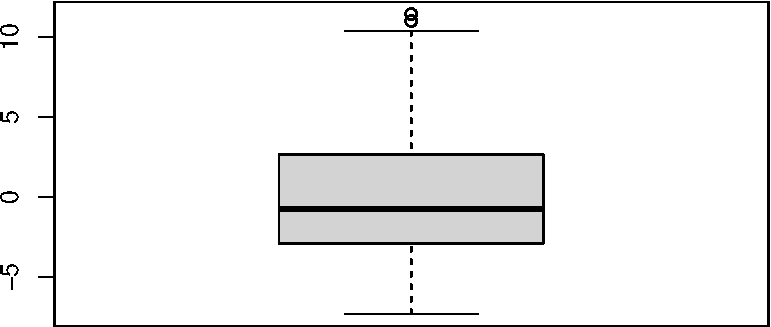
\includegraphics{Longi_mixeffect_files/figure-pdf/unnamed-chunk-6-1.pdf}

}

\end{figure}

\begin{Shaded}
\begin{Highlighting}[]
\CommentTok{\# added {-} some helpful functions}
\FunctionTok{summary}\NormalTok{(}\FunctionTok{resid}\NormalTok{(mod\_1))  }\CommentTok{\# calculate summary statistics of residuals}
\end{Highlighting}
\end{Shaded}

\begin{verbatim}
    Min.  1st Qu.   Median     Mean  3rd Qu.     Max. 
-14.5050  -2.1487  -0.1027   0.0000   2.6309  36.9713 
\end{verbatim}

\begin{Shaded}
\begin{Highlighting}[]
\FunctionTok{hist}\NormalTok{(}\FunctionTok{resid}\NormalTok{(mod\_1))  }\CommentTok{\# create histogram to assess distribution of residuals}
\end{Highlighting}
\end{Shaded}

\begin{figure}[H]

{\centering 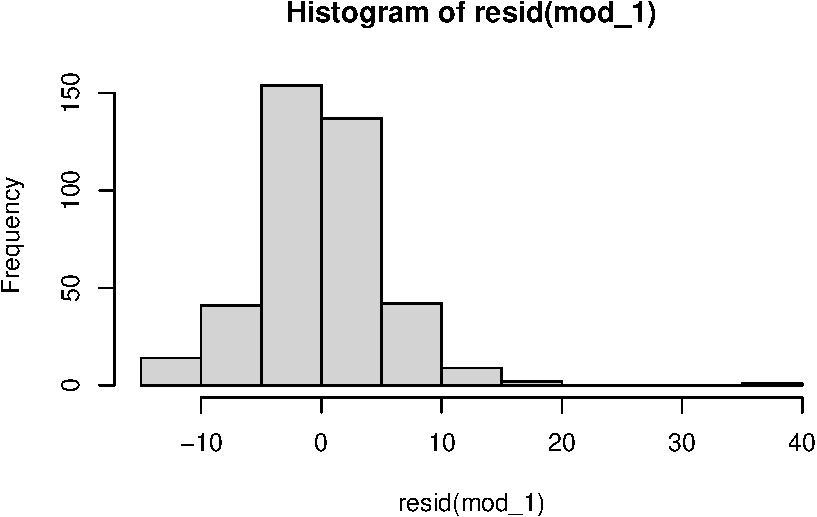
\includegraphics{Longi_mixeffect_files/figure-pdf/unnamed-chunk-7-1.pdf}

}

\end{figure}

\begin{Shaded}
\begin{Highlighting}[]
\CommentTok{\# add plot to visualize individual intercepts using dotplot() from the lattice}
\CommentTok{\# package}
\FunctionTok{dotplot}\NormalTok{(}\FunctionTok{ranef}\NormalTok{(mod\_1))}
\end{Highlighting}
\end{Shaded}

\begin{verbatim}
$id
\end{verbatim}

\begin{figure}[H]

{\centering 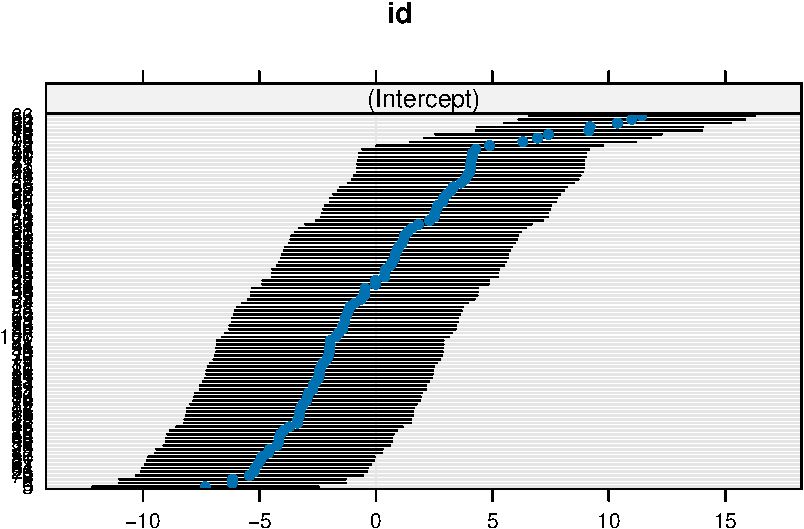
\includegraphics{Longi_mixeffect_files/figure-pdf/unnamed-chunk-8-1.pdf}

}

\end{figure}

\begin{center}
Model 2: $E(y_{ij} \mid X_{ij}) = \beta_0 +  \beta_{trt}trt +  \beta_{T}T + b_{0,i} + b_{T,i}T$
\end{center}

Here the term (1+time\textbar id) specifies the random intercept and
random slope for time.

\begin{Shaded}
\begin{Highlighting}[]
\CommentTok{\# label this model object as mod\_2}
\NormalTok{mod\_2 }\OtherTok{\textless{}{-}} \FunctionTok{lmer}\NormalTok{(measurements }\SpecialCharTok{\textasciitilde{}} \DecValTok{1} \SpecialCharTok{+}\NormalTok{ group }\SpecialCharTok{+}\NormalTok{ time }\SpecialCharTok{+}\NormalTok{ (}\DecValTok{1} \SpecialCharTok{+}\NormalTok{ time }\SpecialCharTok{|}\NormalTok{ id), }\AttributeTok{data =}\NormalTok{ long\_TLC,}
    \AttributeTok{REML =} \ConstantTok{TRUE}\NormalTok{)}
\FunctionTok{summary}\NormalTok{(mod\_2)}
\end{Highlighting}
\end{Shaded}

\begin{verbatim}
Linear mixed model fit by REML ['lmerMod']
Formula: measurements ~ 1 + group + time + (1 + time | id)
   Data: long_TLC

REML criterion at convergence: 2664.4

Scaled residuals: 
    Min      1Q  Median      3Q     Max 
-2.6833 -0.3869 -0.0118  0.4731  5.8022 

Random effects:
 Groups   Name        Variance Std.Dev. Corr
 id       (Intercept) 14.93750 3.8649       
          time         0.09966 0.3157   1.00
 Residual             33.08488 5.7519       
Number of obs: 400, groups:  id, 100

Fixed effects:
               Estimate Std. Error t value
(Intercept)     25.7370     0.7965  32.312
groupTreatment  -5.5220     1.0814  -5.106
time            -0.4010     0.1247  -3.217

Correlation of Fixed Effects:
            (Intr) grpTrt
groupTrtmnt -0.679       
time        -0.280  0.000
optimizer (nloptwrap) convergence code: 0 (OK)
boundary (singular) fit: see help('isSingular')
\end{verbatim}

\begin{center}
Model 3: $E(y_{ij} \mid X_{ij}) = \beta_0 + \beta_{trt}trt + \beta_{T}T + \beta_{trt:T}trt*T + b_{0,i}$
\end{center}

This model includes time as a continuous covariate and also includes an
interaction term to account and adjust for any possible discrepancies
between the treatment and control.

\begin{Shaded}
\begin{Highlighting}[]
\CommentTok{\# label this model object as mod\_3}
\NormalTok{mod\_3 }\OtherTok{\textless{}{-}} \FunctionTok{lmer}\NormalTok{(measurements }\SpecialCharTok{\textasciitilde{}} \DecValTok{1} \SpecialCharTok{+}\NormalTok{ group }\SpecialCharTok{+}\NormalTok{ time }\SpecialCharTok{+}\NormalTok{ group}\SpecialCharTok{:}\NormalTok{time }\SpecialCharTok{+}\NormalTok{ (}\DecValTok{1} \SpecialCharTok{|}\NormalTok{ id), }\AttributeTok{data =}\NormalTok{ long\_TLC,}
    \AttributeTok{REML =} \ConstantTok{TRUE}\NormalTok{)}
\FunctionTok{summary}\NormalTok{(mod\_3)}
\end{Highlighting}
\end{Shaded}

\begin{verbatim}
Linear mixed model fit by REML ['lmerMod']
Formula: measurements ~ 1 + group + time + group:time + (1 | id)
   Data: long_TLC

REML criterion at convergence: 2671.1

Scaled residuals: 
    Min      1Q  Median      3Q     Max 
-2.4683 -0.3762 -0.0182  0.4630  6.3507 

Random effects:
 Groups   Name        Variance Std.Dev.
 id       (Intercept) 22.06    4.697   
 Residual             34.08    5.838   
Number of obs: 400, groups:  id, 100

Fixed effects:
                    Estimate Std. Error t value
(Intercept)         25.68536    0.91553  28.055
groupTreatment      -5.41873    1.29476  -4.185
time                -0.37213    0.17310  -2.150
groupTreatment:time -0.05774    0.24480  -0.236

Correlation of Fixed Effects:
            (Intr) grpTrt time  
groupTrtmnt -0.707              
time        -0.520  0.368       
grpTrtmnt:t  0.368 -0.520 -0.707
\end{verbatim}

\begin{center}
Model 4: $E(y_{ij} \mid X_{ij}) = \beta_0 +  \beta_{trt}trt +  \beta_{T}T + \beta_{trt:T}T*trt+b_{0,i} + b_{T,i}T$
\end{center}

This model treats time as a continuous covariate and also introduces a
quadratic term.

\begin{Shaded}
\begin{Highlighting}[]
\CommentTok{\# label this model object as mod\_4}
\NormalTok{mod\_4 }\OtherTok{\textless{}{-}} \FunctionTok{lmer}\NormalTok{(measurements }\SpecialCharTok{\textasciitilde{}} \DecValTok{1} \SpecialCharTok{+}\NormalTok{ group }\SpecialCharTok{+}\NormalTok{ time }\SpecialCharTok{+}\NormalTok{ time}\SpecialCharTok{:}\NormalTok{group }\SpecialCharTok{+}\NormalTok{ (}\DecValTok{1} \SpecialCharTok{+}\NormalTok{ time }\SpecialCharTok{|}\NormalTok{ id), }\AttributeTok{data =}\NormalTok{ long\_TLC,}
    \AttributeTok{REML =} \ConstantTok{TRUE}\NormalTok{)}
\FunctionTok{summary}\NormalTok{(mod\_4)}
\end{Highlighting}
\end{Shaded}

\begin{verbatim}
Linear mixed model fit by REML ['lmerMod']
Formula: measurements ~ 1 + group + time + time:group + (1 + time | id)
   Data: long_TLC

REML criterion at convergence: 2665.3

Scaled residuals: 
    Min      1Q  Median      3Q     Max 
-2.6754 -0.3847 -0.0057  0.4880  5.8046 

Random effects:
 Groups   Name        Variance Std.Dev. Corr
 id       (Intercept) 14.8608  3.8550       
          time         0.1017  0.3189   1.00
 Residual             33.1807  5.7603       
Number of obs: 400, groups:  id, 100

Fixed effects:
                    Estimate Std. Error t value
(Intercept)         25.68536    0.82687  31.063
groupTreatment      -5.41873    1.16937  -4.634
time                -0.37213    0.17665  -2.107
groupTreatment:time -0.05774    0.24982  -0.231

Correlation of Fixed Effects:
            (Intr) grpTrt time  
groupTrtmnt -0.707              
time        -0.381  0.269       
grpTrtmnt:t  0.269 -0.381 -0.707
optimizer (nloptwrap) convergence code: 0 (OK)
boundary (singular) fit: see help('isSingular')
\end{verbatim}

\begin{center}
Model 5: $E(y_{ij} \mid X_{ij}) = \beta_0 + \beta_{trt}trt + \beta_{T}T + \beta_{T^2}T^2 + \beta_{trt:T}trt*T+\beta_{trt:T^2}trt*T^2+b_{0,i} + b_{T,i}T$
\end{center}

This model includes time as a continuous covariate and also includes a
quadratic term to capture any possible non-linearity in time and an
interaction term to account and adjust for any possible discrepancies
between the treatment and control.

\begin{Shaded}
\begin{Highlighting}[]
\CommentTok{\# label this model object as mod\_5}
\NormalTok{mod\_5 }\OtherTok{\textless{}{-}} \FunctionTok{lmer}\NormalTok{(measurements }\SpecialCharTok{\textasciitilde{}} \DecValTok{1} \SpecialCharTok{+}\NormalTok{ group }\SpecialCharTok{+}\NormalTok{ time }\SpecialCharTok{+} \FunctionTok{I}\NormalTok{(time}\SpecialCharTok{\^{}}\DecValTok{2}\NormalTok{) }\SpecialCharTok{+}\NormalTok{ group}\SpecialCharTok{:}\NormalTok{(time }\SpecialCharTok{+} \FunctionTok{I}\NormalTok{(time}\SpecialCharTok{\^{}}\DecValTok{2}\NormalTok{)) }\SpecialCharTok{+}
\NormalTok{    (}\DecValTok{1} \SpecialCharTok{+}\NormalTok{ time }\SpecialCharTok{|}\NormalTok{ id) }\SpecialCharTok{+}\NormalTok{ (}\FunctionTok{I}\NormalTok{(time}\SpecialCharTok{\^{}}\DecValTok{2}\NormalTok{) }\SpecialCharTok{|}\NormalTok{ id), }\AttributeTok{data =}\NormalTok{ long\_TLC, }\AttributeTok{REML =} \ConstantTok{TRUE}\NormalTok{)}
\FunctionTok{summary}\NormalTok{(mod\_5)}
\end{Highlighting}
\end{Shaded}

\begin{verbatim}
Linear mixed model fit by REML ['lmerMod']
Formula: 
measurements ~ 1 + group + time + I(time^2) + group:(time + I(time^2)) +  
    (1 + time | id) + (I(time^2) | id)
   Data: long_TLC

REML criterion at convergence: 2547.2

Scaled residuals: 
    Min      1Q  Median      3Q     Max 
-3.7766 -0.4184 -0.0564  0.3925  5.9170 

Random effects:
 Groups   Name        Variance Std.Dev. Corr
 id       (Intercept) 16.660   4.0817       
          time         0.114   0.3377   1.00
 id.1     (Intercept)  0.000   0.0000       
          I(time^2)    0.000   0.0000    NaN
 Residual             22.056   4.6964       
Number of obs: 400, groups:  id, 100

Fixed effects:
                         Estimate Std. Error t value
(Intercept)              25.96954    0.82515  31.473
groupTreatment           -1.99607    1.16693  -1.711
time                     -0.91731    0.59637  -1.538
I(time^2)                 0.09170    0.09721   0.943
groupTreatment:time      -6.62390    0.84339  -7.854
groupTreatment:I(time^2)  1.10447    0.13747   8.034

Correlation of Fixed Effects:
            (Intr) grpTrt time   I(t^2) grpTr:
groupTrtmnt -0.707                            
time        -0.406  0.287                     
I(time^2)    0.365 -0.258 -0.969              
grpTrtmnt:t  0.287 -0.406 -0.707  0.685       
grpTr:I(^2) -0.258  0.365  0.685 -0.707 -0.969
optimizer (nloptwrap) convergence code: 0 (OK)
boundary (singular) fit: see help('isSingular')
\end{verbatim}

\begin{Shaded}
\begin{Highlighting}[]
\NormalTok{mod\_5\_test }\OtherTok{\textless{}{-}} \FunctionTok{lmer}\NormalTok{(measurements }\SpecialCharTok{\textasciitilde{}} \DecValTok{1} \SpecialCharTok{+}\NormalTok{ group }\SpecialCharTok{+}\NormalTok{ time }\SpecialCharTok{+} \FunctionTok{I}\NormalTok{(time}\SpecialCharTok{\^{}}\DecValTok{2}\NormalTok{) }\SpecialCharTok{+}\NormalTok{ group}\SpecialCharTok{:}\NormalTok{(time }\SpecialCharTok{+} \FunctionTok{I}\NormalTok{(time}\SpecialCharTok{\^{}}\DecValTok{2}\NormalTok{)) }\SpecialCharTok{+}
\NormalTok{    (}\DecValTok{1} \SpecialCharTok{+}\NormalTok{ time }\SpecialCharTok{+} \FunctionTok{I}\NormalTok{(time}\SpecialCharTok{\^{}}\DecValTok{2}\NormalTok{) }\SpecialCharTok{|}\NormalTok{ id), }\AttributeTok{data =}\NormalTok{ long\_TLC, }\AttributeTok{REML =} \ConstantTok{TRUE}\NormalTok{)}
\FunctionTok{summary}\NormalTok{(mod\_5\_test)}
\end{Highlighting}
\end{Shaded}

\begin{verbatim}
Linear mixed model fit by REML ['lmerMod']
Formula: 
measurements ~ 1 + group + time + I(time^2) + group:(time + I(time^2)) +  
    (1 + time + I(time^2) | id)
   Data: long_TLC

REML criterion at convergence: 2543

Scaled residuals: 
    Min      1Q  Median      3Q     Max 
-3.2531 -0.4033 -0.0512  0.3865  5.2033 

Random effects:
 Groups   Name        Variance Std.Dev. Corr       
 id       (Intercept) 14.6592  3.8287              
          time         3.3089  1.8190    0.49      
          I(time^2)    0.1047  0.3236   -0.28 -0.98
 Residual             19.8761  4.4583              
Number of obs: 400, groups:  id, 100

Fixed effects:
                         Estimate Std. Error t value
(Intercept)               25.9695     0.7788  33.347
groupTreatment            -1.9961     1.1014  -1.812
time                      -0.9173     0.6202  -1.479
I(time^2)                  0.0917     0.1030   0.890
groupTreatment:time       -6.6239     0.8771  -7.552
groupTreatment:I(time^2)   1.1045     0.1457   7.582

Correlation of Fixed Effects:
            (Intr) grpTrt time   I(t^2) grpTr:
groupTrtmnt -0.707                            
time        -0.283  0.200                     
I(time^2)    0.242 -0.171 -0.972              
grpTrtmnt:t  0.200 -0.283 -0.707  0.687       
grpTr:I(^2) -0.171  0.242  0.687 -0.707 -0.972
optimizer (nloptwrap) convergence code: 0 (OK)
boundary (singular) fit: see help('isSingular')
\end{verbatim}

\hypertarget{model-comparison}{%
\section{Model Comparison}\label{model-comparison}}

We are able to compare the models using AIC and BIC. After you write the
other models above, run this chunk below.

\begin{Shaded}
\begin{Highlighting}[]
\NormalTok{Mixed\_Model\_comparisons }\OtherTok{\textless{}{-}} \FunctionTok{data.frame}\NormalTok{(}\StringTok{\textasciigrave{}}\AttributeTok{Model Name}\StringTok{\textasciigrave{}} \OtherTok{=} \FunctionTok{c}\NormalTok{(}\StringTok{"Mixed Model 1"}\NormalTok{, }\StringTok{"Mixed Model 2"}\NormalTok{,}
    \StringTok{"Mixed Model 3"}\NormalTok{, }\StringTok{"Mixed Model 4"}\NormalTok{, }\StringTok{"Mixed Model 5"}\NormalTok{), }\AttributeTok{AIC =} \FunctionTok{c}\NormalTok{(}\FunctionTok{AIC}\NormalTok{(mod\_1), }\FunctionTok{AIC}\NormalTok{(mod\_2),}
    \FunctionTok{AIC}\NormalTok{(mod\_3), }\FunctionTok{AIC}\NormalTok{(mod\_4), }\FunctionTok{AIC}\NormalTok{(mod\_5)), }\AttributeTok{BIC =} \FunctionTok{c}\NormalTok{(}\FunctionTok{BIC}\NormalTok{(mod\_1), }\FunctionTok{BIC}\NormalTok{(mod\_2), }\FunctionTok{BIC}\NormalTok{(mod\_3),}
    \FunctionTok{BIC}\NormalTok{(mod\_4), }\FunctionTok{BIC}\NormalTok{(mod\_5)))}
\NormalTok{Mixed\_Model\_comparisons}
\end{Highlighting}
\end{Shaded}

\begin{verbatim}
     Model.Name      AIC      BIC
1 Mixed Model 1 2680.185 2700.143
2 Mixed Model 2 2678.397 2706.337
3 Mixed Model 3 2683.108 2707.057
4 Mixed Model 4 2681.281 2713.213
5 Mixed Model 5 2573.229 2625.118
\end{verbatim}

Which model would you select?

\textbf{Answer: We would pick Model 5 because it has the lowest AIC and
lowest BIC value.}

\hypertarget{sec-longi-compare}{%
\chapter{Comparison Covariance and Marginal
Model}\label{sec-longi-compare}}

\hypertarget{sec-longi-covmodel}{%
\chapter{Modeling the Covariance}\label{sec-longi-covmodel}}

\begin{Shaded}
\begin{Highlighting}[]
\FunctionTok{library}\NormalTok{(tidyr)  }\CommentTok{\#Allows for us to manipulate the data structure}
\FunctionTok{library}\NormalTok{(data.table)  }\CommentTok{\#Allows for us to manipulate the data structure}
\FunctionTok{library}\NormalTok{(lme4)  }\CommentTok{\#Allows us to fit mixed effects models}
\FunctionTok{library}\NormalTok{(lattice)  }\CommentTok{\#for plotting random effects}
\FunctionTok{library}\NormalTok{(nlme)}
\end{Highlighting}
\end{Shaded}

Recall (from \textcolor{red}{Lab 2} notes): Using the \texttt{gls()}
function to fit a linear model using generalized least squares. The
syntax for the function \texttt{gls()} in \texttt{nlme} package is

gls(model, data, correlation, weights, subset, method, na.action,
control, verbose)

\begin{itemize}
\tightlist
\item
  Description

  \begin{itemize}
  \tightlist
  \item
    \texttt{model}: A two-sided linear formula object describing the
    model
  \item
    \texttt{data}: Optional dataframe
  \item
    \texttt{correlation}: See description for details.

    \begin{itemize}
    \tightlist
    \item
      The \texttt{corStruct} object describes the within-group
      correlation structure.
    \item
      Note we use \texttt{corCompSymm} which has the following syntax:
      corCompSymm(value, form, fixed) compound symmetry structure
      corresponding to a constant correlation.
    \end{itemize}
  \item
    \texttt{weights}: See description for details.

    \begin{itemize}
    \tightlist
    \item
      Describes the variance function.
    \item
      Note we use \texttt{varClasses} which defines standard classes of
      variance function structures and use ``varIdent'' which describes
      constant variance(s), that is generally used to allow different
      variances.
    \end{itemize}
  \end{itemize}
\end{itemize}

Model 1:
\(E(y_{ij} \mid X_{ij}) = \beta_0 + \beta_{trt}trt + \beta_{T_1}T_1 + \beta_{T_4}T_4 + \beta_{T_6}T_6 + \beta_{trt:T_1}trt*T_1 + \beta_{trt:T_4}trt*T_4 + \beta_{trt:T_6}trt*T_6\).

This model includes time as a categorical covariate and also includes an
interaction term to account and adjust for any possible discrepancies
between the treatment and control.

\begin{Shaded}
\begin{Highlighting}[]
\CommentTok{\# unstructured covariance}
\NormalTok{mod\_1\_unstruc }\OtherTok{\textless{}{-}} \FunctionTok{gls}\NormalTok{(measurements }\SpecialCharTok{\textasciitilde{}} \FunctionTok{factor}\NormalTok{(group) }\SpecialCharTok{+} \FunctionTok{factor}\NormalTok{(level) }\SpecialCharTok{+} \FunctionTok{factor}\NormalTok{(group)}\SpecialCharTok{:}\FunctionTok{factor}\NormalTok{(level),}
    \AttributeTok{data =}\NormalTok{ long\_TLC, }\AttributeTok{corr =} \FunctionTok{corSymm}\NormalTok{(}\AttributeTok{form =} \SpecialCharTok{\textasciitilde{}}\DecValTok{1} \SpecialCharTok{|}\NormalTok{ id), }\AttributeTok{weights =} \FunctionTok{varIdent}\NormalTok{(}\AttributeTok{form =} \SpecialCharTok{\textasciitilde{}}\DecValTok{1} \SpecialCharTok{|}
        \FunctionTok{as.factor}\NormalTok{(level)), }\AttributeTok{method =} \StringTok{"REML"}\NormalTok{)}
\FunctionTok{summary}\NormalTok{(mod\_1\_unstruc)}
\end{Highlighting}
\end{Shaded}

\begin{verbatim}
Generalized least squares fit by REML
  Model: measurements ~ factor(group) + factor(level) + factor(group):factor(level) 
  Data: long_TLC 
       AIC      BIC    logLik
  2452.076 2523.559 -1208.038

Correlation Structure: General
 Formula: ~1 | id 
 Parameter estimate(s):
 Correlation: 
  1     2     3    
2 0.571            
3 0.570 0.775      
4 0.577 0.582 0.581
Variance function:
 Structure: Different standard deviations per stratum
 Formula: ~1 | as.factor(level) 
 Parameter estimates:
   lead0    lead1    lead4    lead6 
1.000000 1.325877 1.370471 1.524816 

Coefficients:
                                            Value Std.Error   t-value p-value
(Intercept)                                26.272 0.7102892  36.98775  0.0000
factor(group)Treatment                      0.268 1.0045006   0.26680  0.7898
factor(level)lead1                         -1.612 0.7919151  -2.03557  0.0425
factor(level)lead4                         -2.202 0.8149218  -2.70210  0.0072
factor(level)lead6                         -2.626 0.8885198  -2.95548  0.0033
factor(group)Treatment:factor(level)lead1 -11.406 1.1199371 -10.18450  0.0000
factor(group)Treatment:factor(level)lead4  -8.824 1.1524735  -7.65658  0.0000
factor(group)Treatment:factor(level)lead6  -3.152 1.2565568  -2.50844  0.0125

 Correlation: 
                                          (Intr) fct()T fct()1 fct()4 fct()6
factor(group)Treatment                    -0.707                            
factor(level)lead1                        -0.218  0.154                     
factor(level)lead4                        -0.191  0.135  0.680              
factor(level)lead6                        -0.096  0.068  0.386  0.385       
factor(group)Treatment:factor(level)lead1  0.154 -0.218 -0.707 -0.481 -0.273
factor(group)Treatment:factor(level)lead4  0.135 -0.191 -0.481 -0.707 -0.272
factor(group)Treatment:factor(level)lead6  0.068 -0.096 -0.273 -0.272 -0.707
                                          f()T:()1 f()T:()4
factor(group)Treatment                                     
factor(level)lead1                                         
factor(level)lead4                                         
factor(level)lead6                                         
factor(group)Treatment:factor(level)lead1                  
factor(group)Treatment:factor(level)lead4  0.680           
factor(group)Treatment:factor(level)lead6  0.386    0.385  

Standardized residuals:
       Min         Q1        Med         Q3        Max 
-2.1756516 -0.6849999 -0.1515556  0.5294195  5.6327729 

Residual standard error: 5.022503 
Degrees of freedom: 400 total; 392 residual
\end{verbatim}

\begin{Shaded}
\begin{Highlighting}[]
\CommentTok{\# exchangeable (constant variances)}
\NormalTok{mod\_1\_exch\_const }\OtherTok{\textless{}{-}} \FunctionTok{gls}\NormalTok{(measurements }\SpecialCharTok{\textasciitilde{}} \FunctionTok{factor}\NormalTok{(group) }\SpecialCharTok{+} \FunctionTok{factor}\NormalTok{(level) }\SpecialCharTok{+} \FunctionTok{factor}\NormalTok{(group)}\SpecialCharTok{:}\FunctionTok{factor}\NormalTok{(level),}
    \AttributeTok{data =}\NormalTok{ long\_TLC, }\AttributeTok{corr =} \FunctionTok{corCompSymm}\NormalTok{(}\AttributeTok{form =} \SpecialCharTok{\textasciitilde{}}\FunctionTok{factor}\NormalTok{(level) }\SpecialCharTok{|}\NormalTok{ id), }\AttributeTok{weights =} \FunctionTok{varIdent}\NormalTok{(}\AttributeTok{form =} \SpecialCharTok{\textasciitilde{}}\DecValTok{1}\NormalTok{),}
    \AttributeTok{method =} \StringTok{"REML"}\NormalTok{)}

\FunctionTok{summary}\NormalTok{(mod\_1\_exch\_const)}
\end{Highlighting}
\end{Shaded}

\begin{verbatim}
Generalized least squares fit by REML
  Model: measurements ~ factor(group) + factor(level) + factor(group):factor(level) 
  Data: long_TLC 
       AIC      BIC    logLik
  2480.621 2520.334 -1230.311

Correlation Structure: Compound symmetry
 Formula: ~factor(level) | id 
 Parameter estimate(s):
      Rho 
0.5954401 

Coefficients:
                                            Value Std.Error   t-value p-value
(Intercept)                                26.272 0.9370175 28.037898  0.0000
factor(group)Treatment                      0.268 1.3251428  0.202242  0.8398
factor(level)lead1                         -1.612 0.8428574 -1.912542  0.0565
factor(level)lead4                         -2.202 0.8428574 -2.612541  0.0093
factor(level)lead6                         -2.626 0.8428574 -3.115592  0.0020
factor(group)Treatment:factor(level)lead1 -11.406 1.1919804 -9.568950  0.0000
factor(group)Treatment:factor(level)lead4  -8.824 1.1919804 -7.402807  0.0000
factor(group)Treatment:factor(level)lead6  -3.152 1.1919804 -2.644339  0.0085

 Correlation: 
                                          (Intr) fct()T fct()1 fct()4 fct()6
factor(group)Treatment                    -0.707                            
factor(level)lead1                        -0.450  0.318                     
factor(level)lead4                        -0.450  0.318  0.500              
factor(level)lead6                        -0.450  0.318  0.500  0.500       
factor(group)Treatment:factor(level)lead1  0.318 -0.450 -0.707 -0.354 -0.354
factor(group)Treatment:factor(level)lead4  0.318 -0.450 -0.354 -0.707 -0.354
factor(group)Treatment:factor(level)lead6  0.318 -0.450 -0.354 -0.354 -0.707
                                          f()T:()1 f()T:()4
factor(group)Treatment                                     
factor(level)lead1                                         
factor(level)lead4                                         
factor(level)lead6                                         
factor(group)Treatment:factor(level)lead1                  
factor(group)Treatment:factor(level)lead4  0.500           
factor(group)Treatment:factor(level)lead6  0.500    0.500  

Standardized residuals:
       Min         Q1        Med         Q3        Max 
-2.5147478 -0.6973588 -0.1498707  0.5542798  6.5106947 

Residual standard error: 6.625714 
Degrees of freedom: 400 total; 392 residual
\end{verbatim}

\begin{Shaded}
\begin{Highlighting}[]
\CommentTok{\# exchangeable (heterogeneous variances)}
\NormalTok{mod\_1\_exch\_heter }\OtherTok{\textless{}{-}} \FunctionTok{gls}\NormalTok{(measurements }\SpecialCharTok{\textasciitilde{}} \FunctionTok{factor}\NormalTok{(group) }\SpecialCharTok{+} \FunctionTok{factor}\NormalTok{(level) }\SpecialCharTok{+} \FunctionTok{factor}\NormalTok{(group)}\SpecialCharTok{:}\FunctionTok{factor}\NormalTok{(level),}
    \AttributeTok{data =}\NormalTok{ long\_TLC, }\AttributeTok{corr =} \FunctionTok{corCompSymm}\NormalTok{(}\AttributeTok{form =} \SpecialCharTok{\textasciitilde{}}\FunctionTok{factor}\NormalTok{(level) }\SpecialCharTok{|}\NormalTok{ id), }\AttributeTok{weights =} \FunctionTok{varIdent}\NormalTok{(}\AttributeTok{form =} \SpecialCharTok{\textasciitilde{}}\DecValTok{1} \SpecialCharTok{|}
        \FunctionTok{factor}\NormalTok{(level)), }\AttributeTok{method =} \StringTok{"REML"}\NormalTok{)}

\FunctionTok{summary}\NormalTok{(mod\_1\_exch\_heter)}
\end{Highlighting}
\end{Shaded}

\begin{verbatim}
Generalized least squares fit by REML
  Model: measurements ~ factor(group) + factor(level) + factor(group):factor(level) 
  Data: long_TLC 
      AIC      BIC   logLik
  2459.96 2511.587 -1216.98

Correlation Structure: Compound symmetry
 Formula: ~factor(level) | id 
 Parameter estimate(s):
      Rho 
0.6102708 
Variance function:
 Structure: Different standard deviations per stratum
 Formula: ~1 | factor(level) 
 Parameter estimates:
   lead0    lead1    lead4    lead6 
1.000000 1.279672 1.323197 1.519220 

Coefficients:
                                            Value Std.Error   t-value p-value
(Intercept)                                26.272 0.7237951  36.29757  0.0000
factor(group)Treatment                      0.268 1.0236008   0.26182  0.7936
factor(level)lead1                         -1.612 0.7506796  -2.14739  0.0324
factor(level)lead4                         -2.202 0.7713883  -2.85459  0.0045
factor(level)lead6                         -2.626 0.8726932  -3.00908  0.0028
factor(group)Treatment:factor(level)lead1 -11.406 1.0616213 -10.74394  0.0000
factor(group)Treatment:factor(level)lead4  -8.824 1.0909078  -8.08868  0.0000
factor(group)Treatment:factor(level)lead6  -3.152 1.2341746  -2.55393  0.0110

 Correlation: 
                                          (Intr) fct()T fct()1 fct()4 fct()6
factor(group)Treatment                    -0.707                            
factor(level)lead1                        -0.211  0.149                     
factor(level)lead4                        -0.181  0.128  0.402              
factor(level)lead6                        -0.060  0.043  0.383  0.383       
factor(group)Treatment:factor(level)lead1  0.149 -0.211 -0.707 -0.285 -0.270
factor(group)Treatment:factor(level)lead4  0.128 -0.181 -0.285 -0.707 -0.271
factor(group)Treatment:factor(level)lead6  0.043 -0.060 -0.270 -0.271 -0.707
                                          f()T:()1 f()T:()4
factor(group)Treatment                                     
factor(level)lead1                                         
factor(level)lead4                                         
factor(level)lead6                                         
factor(group)Treatment:factor(level)lead1                  
factor(group)Treatment:factor(level)lead4  0.402           
factor(group)Treatment:factor(level)lead6  0.383    0.383  

Standardized residuals:
       Min         Q1        Med         Q3        Max 
-2.1429199 -0.6927789 -0.1528885  0.5263121  5.5480303 

Residual standard error: 5.118004 
Degrees of freedom: 400 total; 392 residual
\end{verbatim}

\hypertarget{sec-longi-modelselection}{%
\chapter{Model Selection}\label{sec-longi-modelselection}}

\begin{Shaded}
\begin{Highlighting}[]
\FunctionTok{library}\NormalTok{(tidyr)  }\CommentTok{\#Allows for us to manipulate the data structure}
\FunctionTok{library}\NormalTok{(data.table)  }\CommentTok{\#Allows for us to manipulate the data structure}
\FunctionTok{library}\NormalTok{(lme4)  }\CommentTok{\#Allows us to fit mixed effects models}
\FunctionTok{library}\NormalTok{(lattice)  }\CommentTok{\#for plotting random effects}
\FunctionTok{library}\NormalTok{(nlme)}
\end{Highlighting}
\end{Shaded}

\hypertarget{comparing-mean-models}{%
\section{Comparing Mean Models}\label{comparing-mean-models}}

In this section, we will apply the backward selection method to

Mod\_base:
\(E(y_{ij} \mid X_{ij}) = \beta_0 + \beta_{trt}trt + \beta_{T}T + \beta_{T^2}T^2 + \beta_{trt:T}trt*T+\beta_{trt:T^2}trt*T^2\).

\begin{Shaded}
\begin{Highlighting}[]
\CommentTok{\# start off with baseline model including all terms}
\NormalTok{mod\_base\_unstruc }\OtherTok{\textless{}{-}} \FunctionTok{gls}\NormalTok{(measurements }\SpecialCharTok{\textasciitilde{}} \FunctionTok{factor}\NormalTok{(group) }\SpecialCharTok{+}\NormalTok{ time }\SpecialCharTok{+} \FunctionTok{I}\NormalTok{(time}\SpecialCharTok{\^{}}\DecValTok{2}\NormalTok{) }\SpecialCharTok{+} \FunctionTok{factor}\NormalTok{(group)}\SpecialCharTok{:}\NormalTok{(time }\SpecialCharTok{+}
    \FunctionTok{I}\NormalTok{(time}\SpecialCharTok{\^{}}\DecValTok{2}\NormalTok{)), }\AttributeTok{data =}\NormalTok{ long\_TLC, }\AttributeTok{corr =} \FunctionTok{corSymm}\NormalTok{(}\AttributeTok{form =} \SpecialCharTok{\textasciitilde{}}\DecValTok{1} \SpecialCharTok{|}\NormalTok{ id), }\AttributeTok{weights =} \FunctionTok{varIdent}\NormalTok{(}\AttributeTok{form =} \SpecialCharTok{\textasciitilde{}}\DecValTok{1} \SpecialCharTok{|}
\NormalTok{    time), }\AttributeTok{method =} \StringTok{"REML"}\NormalTok{)}

\FunctionTok{summary}\NormalTok{(mod\_base\_unstruc)}
\end{Highlighting}
\end{Shaded}

\begin{verbatim}
Generalized least squares fit by REML
  Model: measurements ~ factor(group) + time + I(time^2) + factor(group):(time +      I(time^2)) 
  Data: long_TLC 
       AIC     BIC    logLik
  2551.458 2615.08 -1259.729

Correlation Structure: General
 Formula: ~1 | id 
 Parameter estimate(s):
 Correlation: 
  1     2     3    
2 0.383            
3 0.554 0.674      
4 0.479 0.645 0.561
Variance function:
 Structure: Different standard deviations per stratum
 Formula: ~1 | time 
 Parameter estimates:
       0        1        4        6 
1.000000 1.559260 1.353064 1.599957 

Coefficients:
                                     Value Std.Error  t-value p-value
(Intercept)                      26.131925 0.7026920 37.18830  0.0000
factor(group)Treatment           -0.780544 0.9937566 -0.78545  0.4327
time                             -0.833454 0.5657092 -1.47329  0.1415
I(time^2)                         0.082735 0.0983326  0.84138  0.4006
factor(group)Treatment:time      -5.996162 0.8000336 -7.49489  0.0000
factor(group)Treatment:I(time^2)  1.037344 0.1390633  7.45951  0.0000

 Correlation: 
                                 (Intr) fct()T time   I(t^2) fc()T:
factor(group)Treatment           -0.707                            
time                             -0.169  0.119                     
I(time^2)                         0.156 -0.110 -0.976              
factor(group)Treatment:time       0.119 -0.169 -0.707  0.690       
factor(group)Treatment:I(time^2) -0.110  0.156  0.690 -0.707 -0.976

Standardized residuals:
       Min         Q1        Med         Q3        Max 
-2.5279798 -0.7879764 -0.2643423  0.4368118  4.8117601 

Residual standard error: 5.092279 
Degrees of freedom: 400 total; 394 residual
\end{verbatim}

\begin{Shaded}
\begin{Highlighting}[]
\CommentTok{\# If there were higher order terms that were significant we would remove them,}
\CommentTok{\# but in this case both interaction terms are significant so we want to keep}
\CommentTok{\# them in the model}

\CommentTok{\# However, suppose the quadratic terms were not significant, lets remove them}
\CommentTok{\# here in this example}
\NormalTok{mod\_second\_unstruc }\OtherTok{\textless{}{-}} \FunctionTok{gls}\NormalTok{(measurements }\SpecialCharTok{\textasciitilde{}} \FunctionTok{factor}\NormalTok{(group) }\SpecialCharTok{+}\NormalTok{ time }\SpecialCharTok{+} \FunctionTok{factor}\NormalTok{(group)}\SpecialCharTok{:}\NormalTok{(time),}
    \AttributeTok{data =}\NormalTok{ long\_TLC, }\AttributeTok{corr =} \FunctionTok{corSymm}\NormalTok{(}\AttributeTok{form =} \SpecialCharTok{\textasciitilde{}}\DecValTok{1} \SpecialCharTok{|}\NormalTok{ id), }\AttributeTok{weights =} \FunctionTok{varIdent}\NormalTok{(}\AttributeTok{form =} \SpecialCharTok{\textasciitilde{}}\DecValTok{1} \SpecialCharTok{|}
\NormalTok{        time), }\AttributeTok{method =} \StringTok{"REML"}\NormalTok{)}

\FunctionTok{summary}\NormalTok{(mod\_second\_unstruc)}
\end{Highlighting}
\end{Shaded}

\begin{verbatim}
Generalized least squares fit by REML
  Model: measurements ~ factor(group) + time + factor(group):(time) 
  Data: long_TLC 
       AIC      BIC    logLik
  2586.646 2642.386 -1279.323

Correlation Structure: General
 Formula: ~1 | id 
 Parameter estimate(s):
 Correlation: 
  1     2     3    
2 0.132            
3 0.271 0.846      
4 0.543 0.406 0.495
Variance function:
 Structure: Different standard deviations per stratum
 Formula: ~1 | time 
 Parameter estimates:
       0        1        4        6 
1.000000 1.833984 1.551842 1.439514 

Coefficients:
                                Value Std.Error  t-value p-value
(Intercept)                 26.039582 0.6940593 37.51780  0.0000
factor(group)Treatment      -1.938410 0.9815481 -1.97485  0.0490
time                        -0.368743 0.1223416 -3.01404  0.0027
factor(group)Treatment:time -0.169559 0.1730172 -0.98001  0.3277

 Correlation: 
                            (Intr) fct()T time  
factor(group)Treatment      -0.707              
time                        -0.077  0.054       
factor(group)Treatment:time  0.054 -0.077 -0.707

Standardized residuals:
       Min         Q1        Med         Q3        Max 
-2.2991338 -0.7973523 -0.2854752  0.3570825  5.6284768 

Residual standard error: 5.310688 
Degrees of freedom: 400 total; 396 residual
\end{verbatim}

Note that all terms are now significant, including the interaction term.
We used the backwards selection method to obtain the ``best'' model.
Suppose we wanted to compare the mean models of mod\_base\_unstruc and
mod\_second\_unstruc. We can compare model means using anova()

\begin{Shaded}
\begin{Highlighting}[]
\FunctionTok{anova}\NormalTok{(mod\_base\_unstruc, mod\_second\_unstruc)}
\end{Highlighting}
\end{Shaded}

\begin{verbatim}
                   Model df      AIC      BIC    logLik   Test  L.Ratio p-value
mod_base_unstruc       1 16 2551.458 2615.080 -1259.729                        
mod_second_unstruc     2 14 2586.646 2642.386 -1279.323 1 vs 2 39.18782  <.0001
\end{verbatim}

Based on these results, which is the best model?

\textbf{Answer: The model called ``mod\_base\_unstruc'' is the best
model which is consistent with our previous results}

\hypertarget{comparing-covariance-models}{%
\section{Comparing Covariance
Models}\label{comparing-covariance-models}}

In previous section, we fit three models on our data using various
covariance structure below:

\begin{Shaded}
\begin{Highlighting}[]
\CommentTok{\# unstructured covariance}
\NormalTok{mod\_1\_unstruc }\OtherTok{\textless{}{-}} \FunctionTok{gls}\NormalTok{(measurements }\SpecialCharTok{\textasciitilde{}} \FunctionTok{factor}\NormalTok{(group) }\SpecialCharTok{+} \FunctionTok{factor}\NormalTok{(level) }\SpecialCharTok{+} \FunctionTok{factor}\NormalTok{(group)}\SpecialCharTok{:}\FunctionTok{factor}\NormalTok{(level),}
    \AttributeTok{data =}\NormalTok{ long\_TLC, }\AttributeTok{corr =} \FunctionTok{corSymm}\NormalTok{(}\AttributeTok{form =} \SpecialCharTok{\textasciitilde{}}\DecValTok{1} \SpecialCharTok{|}\NormalTok{ id), }\AttributeTok{weights =} \FunctionTok{varIdent}\NormalTok{(}\AttributeTok{form =} \SpecialCharTok{\textasciitilde{}}\DecValTok{1} \SpecialCharTok{|}
        \FunctionTok{as.factor}\NormalTok{(level)), }\AttributeTok{method =} \StringTok{"REML"}\NormalTok{)}

\CommentTok{\# exchangeable (constant variances)}
\NormalTok{mod\_1\_exch\_const }\OtherTok{\textless{}{-}} \FunctionTok{gls}\NormalTok{(measurements }\SpecialCharTok{\textasciitilde{}} \FunctionTok{factor}\NormalTok{(group) }\SpecialCharTok{+} \FunctionTok{factor}\NormalTok{(level) }\SpecialCharTok{+} \FunctionTok{factor}\NormalTok{(group)}\SpecialCharTok{:}\FunctionTok{factor}\NormalTok{(level),}
    \AttributeTok{data =}\NormalTok{ long\_TLC, }\AttributeTok{corr =} \FunctionTok{corCompSymm}\NormalTok{(}\AttributeTok{form =} \SpecialCharTok{\textasciitilde{}}\FunctionTok{factor}\NormalTok{(level) }\SpecialCharTok{|}\NormalTok{ id), }\AttributeTok{weights =} \FunctionTok{varIdent}\NormalTok{(}\AttributeTok{form =} \SpecialCharTok{\textasciitilde{}}\DecValTok{1}\NormalTok{),}
    \AttributeTok{method =} \StringTok{"REML"}\NormalTok{)}

\CommentTok{\# exchangeable (heterogeneous variances)}
\NormalTok{mod\_1\_exch\_heter }\OtherTok{\textless{}{-}} \FunctionTok{gls}\NormalTok{(measurements }\SpecialCharTok{\textasciitilde{}} \FunctionTok{factor}\NormalTok{(group) }\SpecialCharTok{+} \FunctionTok{factor}\NormalTok{(level) }\SpecialCharTok{+} \FunctionTok{factor}\NormalTok{(group)}\SpecialCharTok{:}\FunctionTok{factor}\NormalTok{(level),}
    \AttributeTok{data =}\NormalTok{ long\_TLC, }\AttributeTok{corr =} \FunctionTok{corCompSymm}\NormalTok{(}\AttributeTok{form =} \SpecialCharTok{\textasciitilde{}}\FunctionTok{factor}\NormalTok{(level) }\SpecialCharTok{|}\NormalTok{ id), }\AttributeTok{weights =} \FunctionTok{varIdent}\NormalTok{(}\AttributeTok{form =} \SpecialCharTok{\textasciitilde{}}\DecValTok{1} \SpecialCharTok{|}
        \FunctionTok{factor}\NormalTok{(level)), }\AttributeTok{method =} \StringTok{"REML"}\NormalTok{)}
\end{Highlighting}
\end{Shaded}

We can compare these models using \texttt{anova}.

\begin{Shaded}
\begin{Highlighting}[]
\CommentTok{\# compare three models together}
\FunctionTok{anova}\NormalTok{(mod\_1\_unstruc, mod\_1\_exch\_const, mod\_1\_exch\_heter)}
\end{Highlighting}
\end{Shaded}

\begin{verbatim}
                 Model df      AIC      BIC    logLik   Test  L.Ratio p-value
mod_1_unstruc        1 18 2452.076 2523.559 -1208.038                        
mod_1_exch_const     2 10 2480.621 2520.334 -1230.311 1 vs 2 44.54508  <.0001
mod_1_exch_heter     3 13 2459.960 2511.587 -1216.980 2 vs 3 26.66058  <.0001
\end{verbatim}

\begin{Shaded}
\begin{Highlighting}[]
\CommentTok{\# or compare two models at a time}
\FunctionTok{anova}\NormalTok{(mod\_1\_unstruc, mod\_1\_exch\_const)}
\end{Highlighting}
\end{Shaded}

\begin{verbatim}
                 Model df      AIC      BIC    logLik   Test  L.Ratio p-value
mod_1_unstruc        1 18 2452.076 2523.559 -1208.038                        
mod_1_exch_const     2 10 2480.621 2520.334 -1230.311 1 vs 2 44.54508  <.0001
\end{verbatim}

\begin{Shaded}
\begin{Highlighting}[]
\FunctionTok{anova}\NormalTok{(mod\_1\_exch\_const, mod\_1\_exch\_heter)}
\end{Highlighting}
\end{Shaded}

\begin{verbatim}
                 Model df      AIC      BIC   logLik   Test  L.Ratio p-value
mod_1_exch_const     1 10 2480.621 2520.334 -1230.31                        
mod_1_exch_heter     2 13 2459.960 2511.587 -1216.98 1 vs 2 26.66058  <.0001
\end{verbatim}

For model selection, we want to compare AIC and BIC. The model with the
unstructured covariance (e.g., mod\_1\_unstruc) has the lowest AIC. The
model with the exchangeable (heterogeneous variances) (e.g.,
mod\_1\_exch\_heter) has the lowest BIC. These results suggest that the
exchangeable (heterogeneous variances) fits the data best since it is
more parsimonious and has low information. Based on the likelihood ratio
test, the mod\_1\_exch\_heter model is a significantly better fit than
the other two models.

\hypertarget{sec-longi-prediction}{%
\chapter{Prediction}\label{sec-longi-prediction}}

\hypertarget{sec-longi-interpretation}{%
\chapter{Interpretation}\label{sec-longi-interpretation}}

ibgdvnbvolnhadv

\hypertarget{intercept}{%
\section{Intercept}\label{intercept}}

\hypertarget{sec-longi-noncontinuous}{%
\chapter{Models for Non-Continuous
Outcomes}\label{sec-longi-noncontinuous}}

\textbf{Learning Objectives}

\begin{enumerate}
\def\labelenumi{\arabic{enumi}.}
\tightlist
\item
  Understand how to conduct fit models with non-continuous outcomes
\item
  Understand how to interpret results
\end{enumerate}

\hypertarget{background}{%
\section{Background}\label{background}}

The purpose of this lab is to learn how to use R software to fit
regression models for longitudinal data when the outcome is
non-continuous. We will discuss Marginal and Mixed-Effects models.

There are two main types of non-continuous outcomes. The first outcome,
which will be the focus of this lab, are binary outcomes where the
response variable \(Y \in \{0,1\}\). For examples consider the
scenarios: Predict whether or not a person will have diabetes or not,
predict whether or not a person is positive for COVID-19 or not.

The response variable is dichotomous coded with 0's and 1's, where
observations labeled as 1's represent the occurrence of an event or
outcome of interest. Observations labeled with 0 are labeled as
belonging to the negative class, where the event or outcome was not
observed.

Here we only have two options which is usually why it's a popular
approach to build probabilistic models \(P(Y=1 \mid X)=g^{-1}(X\beta)\)
to model the outcome. g is what we call a link function, and common link
functions are the logistic link function \(g(p) = log(\frac{p}{1-p})\),
the standard normal cumulative density function \(\Phi(p)\), and the
complementary log-log function \(g(p) = log(-log(1-p))\). log refers to
the natural log.

For these outcomes, we need to build probabilistic models. Why? Because
we cannot use a linear model to estimate the classes. We cannot
interpret the output of a linear regression model with these
non-continuous outcomes.

Statisticians prefer probabilistic estimation as it gives us a way to
quantify an individual's level of association to a certain occurrence of
event. Probabilities are always bounded between 0 and 1. This
boundedness property allows us to know for certain how extreme your
estimates are. For instance if your predicted probability is 0.90 then
you know there's an extremely high chance this individual belongs to the
positive class. If \(P(Y=1 \mid X)\) is high (e.g.~greater than 0.5)
then we say it's more likely that they're in the positive class than in
the negative class. As an aside, but not relevant to the lab, this can
also be extended to categorical outcomes where instead of two outcomes
there are K outcomes, where \(K \ge 2\) (i.e.~multinomial logistic
regression). We will not discuss this further.

Another type of non-continuous outcome variable takes on discrete values
(i.e.~integer values like 0,1,2,3,\dots). This is defined as ``count
data'' which represents the number of occurrences of an event within a
fixed period. Examples include the number of accidents on a freeway over
a year or number of cancer cases in a month. Usually models with count
responses are estimated using, though not limited to, Poisson and
Negative Binomial distributions.

The main rules that we learnt in previous labs for continuous outcomes
also apply for non-continuous outcomes. For instance Marginal models for
non-continuous outcomes are also population level while Mixed Effect
models for non-continuous outcomes are individual (or subject-specific)
level.

Analogous overall model-selection procedures also remain the same. For
instance when doing Maximum Likelihood Estimation we can still use the
Akaike Information Criterion (AIC) and the Bayesian Information
Criterion (BIC) to select our final model. For reference
\(AIC = 2p - 2log(L)\) where \(L\) is the likelihood and p is the number
of covariates (excluding the intercept). Similarly
\(BIC = plog(n) - 2log(L)\) where n is the sample size of the data.

While model comparisons remain the same we need to be careful when
intepreting the coefficients that we derive from such models. There is a
non-linear relationship being imposed now and we need to adjust our
understanding accordlingly. Of course though the above sentence needs
some explanation for one to truly grasp what the difference is. In a
linear regression \(y = X^T\beta\) so we'd interpret the \(\beta\) in
relation to the response. In logistic regression,
\(logit(p) = log(\frac{p}{1-p}) = X^T\beta\) this \(\beta\) represents
how a covariate affects the log-odds. An easier way to interpret
\(\beta\) in terms of \(e^\beta\) which then tells us how it affects the
odds ratio \(\frac{p}{1-p}\).

\hypertarget{introduction-2}{%
\section{Introduction}\label{introduction-2}}

In this lab, we will use data from the ``Muscatine Coronary Risk Factor
Study'' (``muscatine.csv'' or ``muscatine.dta''). The goal of the study
was to examine the development and persistence of risk factors for
coronary disease in children. Below we describe our data.

The outcome of interest: Obesity status (binary response,
``obesity\_status'').

The data is longitudinal with each subject having at most three
measurements. Measurements were taken biannually (every two years) from
1977 to 1981 (i.e.~1977, 1979, 1981). You'll notice the dataset is
already in long format. This is captured in the occasion variable (``1''
= 1977, ``2'' = 1979, ``3'' = 1981).

\textbf{Covariates of interest:} Current age (``curr\_age''), baseline
age (``base\_age'') and gender (``gender''). There is also an id
variable (``id'') specific to each participant within the study.

\textbf{Main Objective:} Determine whether the risk of obesity increases
with age, and whether the patterns of change in obesity are the same for
boys and girls.

\begin{itemize}
\tightlist
\item
  We will use the following packages for models:

  \begin{itemize}
  \tightlist
  \item
    lme4: This package is for fitting mixed-effects models. We will use
    the lmer() function to fit a linear model.
  \item
    geepack: This is the ``Generalized Estimating Equation Package''
    package
  \end{itemize}
\end{itemize}

\hypertarget{loading-the-data-into-rstudio}{%
\section{Loading the Data into
RStudio}\label{loading-the-data-into-rstudio}}

\begin{Shaded}
\begin{Highlighting}[]
\FunctionTok{library}\NormalTok{(tidyr)  }\CommentTok{\# To manipulate the data structure}
\FunctionTok{library}\NormalTok{(data.table)  }\CommentTok{\# To manipulate the data structure}
\FunctionTok{library}\NormalTok{(ggplot2)  }\CommentTok{\# To create plots}
\FunctionTok{library}\NormalTok{(dplyr)  }\CommentTok{\#for dataset manipulations with the \%\textgreater{}\% operator}
\FunctionTok{library}\NormalTok{(scales)  }\CommentTok{\#for making percentages appear on y axis in ggplot}
\FunctionTok{library}\NormalTok{(naniar)  }\CommentTok{\#for missing data visualizations}

\CommentTok{\# packages for models}
\FunctionTok{library}\NormalTok{(lme4)  }\CommentTok{\# for mixed effects models}
\FunctionTok{library}\NormalTok{(geepack)  }\CommentTok{\# install.packages(\textquotesingle{}geepack\textquotesingle{}), used for the geeglm() function}
\end{Highlighting}
\end{Shaded}

\begin{Shaded}
\begin{Highlighting}[]
\DocumentationTok{\#\# SLOWEST METHOD: This is in base R (i.e. you odn\textquotesingle{}t need to load any packages)}
\NormalTok{muscatine }\OtherTok{\textless{}{-}} \FunctionTok{read.csv}\NormalTok{(}\StringTok{"Data/muscatine.csv"}\NormalTok{)}
\CommentTok{\# head function allows us to see a sneak preview of the data.}
\FunctionTok{head}\NormalTok{(muscatine, }\AttributeTok{n =} \DecValTok{10}\NormalTok{)}
\end{Highlighting}
\end{Shaded}

\begin{verbatim}
   id gender base_age curr_age occasion obesity_status
1   1      0        6        6        1              1
2   1      0        6        8        2              1
3   1      0        6       10        3              1
4   2      0        6        6        1              1
5   2      0        6        8        2              1
6   2      0        6       10        3              1
7   3      0        6        6        1              1
8   3      0        6        8        2              1
9   3      0        6       10        3              1
10  4      0        6        6        1              1
\end{verbatim}

Below we standardize the current age variable by centering by the mean.
We also create a label for the gender variable.

\begin{Shaded}
\begin{Highlighting}[]
\CommentTok{\# Here we turn muscatine into a data table for easier manipulations}
\NormalTok{muscatine }\OtherTok{\textless{}{-}} \FunctionTok{data.table}\NormalTok{(muscatine)}
\CommentTok{\# Center the variable age (curr\_age) around the mean}
\NormalTok{muscatine[, centered\_age }\SpecialCharTok{:}\ErrorTok{=}\NormalTok{ curr\_age }\SpecialCharTok{{-}} \FunctionTok{mean}\NormalTok{(curr\_age)]}
\CommentTok{\# create labels for gender variable}
\NormalTok{muscatine[, gender\_label }\SpecialCharTok{:}\ErrorTok{=} \FunctionTok{ifelse}\NormalTok{(gender }\SpecialCharTok{==} \DecValTok{0}\NormalTok{, }\StringTok{"male"}\NormalTok{, }\StringTok{"female"}\NormalTok{)]}

\FunctionTok{head}\NormalTok{(muscatine, }\AttributeTok{n =} \DecValTok{10}\NormalTok{)}
\end{Highlighting}
\end{Shaded}

\begin{verbatim}
       id gender base_age curr_age occasion obesity_status centered_age
    <int>  <int>    <int>    <int>    <int>          <int>        <num>
 1:     1      0        6        6        1              1    -5.976524
 2:     1      0        6        8        2              1    -3.976524
 3:     1      0        6       10        3              1    -1.976524
 4:     2      0        6        6        1              1    -5.976524
 5:     2      0        6        8        2              1    -3.976524
 6:     2      0        6       10        3              1    -1.976524
 7:     3      0        6        6        1              1    -5.976524
 8:     3      0        6        8        2              1    -3.976524
 9:     3      0        6       10        3              1    -1.976524
10:     4      0        6        6        1              1    -5.976524
    gender_label
          <char>
 1:         male
 2:         male
 3:         male
 4:         male
 5:         male
 6:         male
 7:         male
 8:         male
 9:         male
10:         male
\end{verbatim}

\hypertarget{exploratory-data-analysis}{%
\section{Exploratory Data Analysis}\label{exploratory-data-analysis}}

Before heading to the model fitting, we first would like to perform some
data exploration to have a better understanding. Firstly we will begin
with a missing data visualization using the \texttt{naniar} package. The
\texttt{naniar} package contains a function called \texttt{vis\_miss}
which allows us to see which covariates are missing data and by how
much. Be sure to install the \texttt{naniar} package first.

\begin{Shaded}
\begin{Highlighting}[]
\FunctionTok{vis\_miss}\NormalTok{(muscatine)}
\end{Highlighting}
\end{Shaded}

\begin{figure}[H]

{\centering 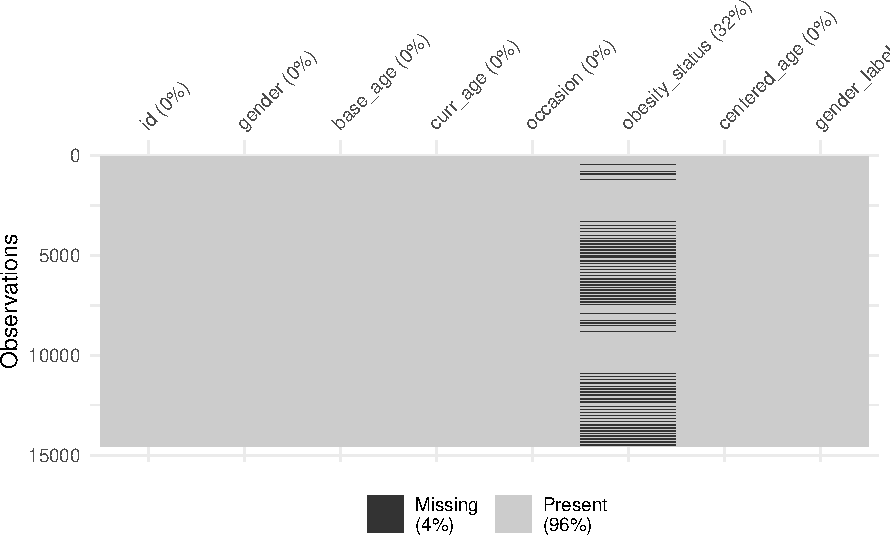
\includegraphics{Longi_noncontinuous_files/figure-pdf/unnamed-chunk-6-1.pdf}

}

\end{figure}

From the above plot we can see that our only missingness is due to the
outcome, obesity status.

\begin{Shaded}
\begin{Highlighting}[]
\NormalTok{muscatine[, numbered\_visit }\SpecialCharTok{:}\ErrorTok{=} \FunctionTok{seq\_len}\NormalTok{(.N), by }\OtherTok{=}\NormalTok{ id]}
\NormalTok{descript }\OtherTok{\textless{}{-}}\NormalTok{ muscatine }\SpecialCharTok{\%\textgreater{}\%}
    \FunctionTok{group\_by}\NormalTok{(numbered\_visit) }\SpecialCharTok{\%\textgreater{}\%}
    \FunctionTok{summarise}\NormalTok{(}\AttributeTok{ids =} \FunctionTok{length}\NormalTok{(id), }\AttributeTok{Males =} \FunctionTok{sum}\NormalTok{(gender\_label }\SpecialCharTok{==} \StringTok{"male"}\NormalTok{), }\AttributeTok{Females =} \FunctionTok{sum}\NormalTok{(gender\_label }\SpecialCharTok{==}
        \StringTok{"female"}\NormalTok{), }\AttributeTok{mean\_age =} \FunctionTok{round}\NormalTok{(}\FunctionTok{mean}\NormalTok{(curr\_age, }\AttributeTok{na.rm =}\NormalTok{ T), }\DecValTok{3}\NormalTok{), }\AttributeTok{sd =} \FunctionTok{round}\NormalTok{(}\FunctionTok{sd}\NormalTok{(curr\_age,}
        \AttributeTok{na.rm =}\NormalTok{ T), }\DecValTok{3}\NormalTok{), }\AttributeTok{var =} \FunctionTok{round}\NormalTok{(}\FunctionTok{var}\NormalTok{(curr\_age, }\AttributeTok{na.rm =}\NormalTok{ T), }\DecValTok{3}\NormalTok{))}
\NormalTok{descript}
\end{Highlighting}
\end{Shaded}

\begin{verbatim}
# A tibble: 3 x 7
  numbered_visit   ids Males Females mean_age    sd   var
           <int> <int> <int>   <int>    <dbl> <dbl> <dbl>
1              1  4856  2486    2370     9.98  2.79  7.80
2              2  4856  2486    2370    12.0   2.79  7.80
3              3  4856  2486    2370    14.0   2.79  7.80
\end{verbatim}

Now we will make barplots to summarize/visualize the proportion of
children who are classified as obese within each age within each gender.
To start we need to derive this proportion variable. ggplot
unfortunately does not have a built in way to specify this so we need to
create a new data frame which can take care of this for us. To do so we
wil be using the dplyr function.

\begin{Shaded}
\begin{Highlighting}[]
\CommentTok{\# by subject, summarize the proportion of these T/F combinations}
\NormalTok{obesity\_prop\_by\_age }\OtherTok{\textless{}{-}}\NormalTok{ muscatine }\SpecialCharTok{\%\textgreater{}\%}
    \CommentTok{\# create a unique identifier for each combination (e.g. \textquotesingle{}TRUE{-}TRUE{-}FALSE\textquotesingle{})}
\FunctionTok{group\_by}\NormalTok{(base\_age, gender\_label) }\SpecialCharTok{\%\textgreater{}\%}
    \CommentTok{\# prop of times each combo type occurs for a given subject:}
\FunctionTok{reframe}\NormalTok{(}\AttributeTok{prop =} \FunctionTok{mean}\NormalTok{(obesity\_status, }\AttributeTok{na.rm =}\NormalTok{ T), }\AttributeTok{times =} \FunctionTok{n}\NormalTok{())}
\end{Highlighting}
\end{Shaded}

Now that we have the proportions for each age group we create a new
variable.

\begin{Shaded}
\begin{Highlighting}[]
\NormalTok{bars }\OtherTok{\textless{}{-}} \FunctionTok{ggplot}\NormalTok{(obesity\_prop\_by\_age,}
        \FunctionTok{aes}\NormalTok{(}\AttributeTok{x =}\NormalTok{ base\_age,}\AttributeTok{y =}\NormalTok{ prop, }\AttributeTok{fill =}\NormalTok{ gender\_label)) }\SpecialCharTok{+} 
  \FunctionTok{geom\_bar}\NormalTok{(}\AttributeTok{stat =} \StringTok{"identity"}\NormalTok{) }\SpecialCharTok{+}
  \FunctionTok{facet\_wrap}\NormalTok{(.}\SpecialCharTok{\textasciitilde{}}\NormalTok{gender\_label) }\SpecialCharTok{+} \CommentTok{\#this is what allows us to make separate boxes for the groups}
  \FunctionTok{theme}\NormalTok{(}\AttributeTok{axis.line =} \FunctionTok{element\_line}\NormalTok{(}\AttributeTok{colour =} \StringTok{"black"}\NormalTok{, }\AttributeTok{linewidth =} \DecValTok{2}\NormalTok{),}
        \AttributeTok{text =} \FunctionTok{element\_text}\NormalTok{(}\AttributeTok{size =} \DecValTok{20}\NormalTok{),}
        \AttributeTok{axis.text =} \FunctionTok{element\_text}\NormalTok{(}\AttributeTok{colour =} \StringTok{"black"}\NormalTok{, }\AttributeTok{size =} \DecValTok{20}\NormalTok{, }\AttributeTok{face =} \StringTok{"bold"}\NormalTok{),}
        \AttributeTok{axis.title =} \FunctionTok{element\_text}\NormalTok{(}\AttributeTok{size =} \DecValTok{24}\NormalTok{, }\AttributeTok{face =} \StringTok{"bold"}\NormalTok{),}
        \AttributeTok{axis.ticks.length =} \FunctionTok{unit}\NormalTok{(.}\DecValTok{25}\NormalTok{, }\StringTok{"cm"}\NormalTok{),}
        \AttributeTok{axis.ticks =} \FunctionTok{element\_line}\NormalTok{(}\AttributeTok{colour =} \StringTok{"black"}\NormalTok{, }\AttributeTok{linewidth =} \FloatTok{1.5}\NormalTok{),}
        \AttributeTok{strip.background=}\FunctionTok{element\_rect}\NormalTok{(}\AttributeTok{colour =} \StringTok{"black"}\NormalTok{, }\AttributeTok{fill =} \StringTok{"yellow"}\NormalTok{)) }\SpecialCharTok{+}
  \FunctionTok{ggtitle}\NormalTok{(}\StringTok{"Proportion of Obese Children by Age and Gender"}\NormalTok{) }\SpecialCharTok{+}
  \FunctionTok{scale\_fill\_manual}\NormalTok{(}\AttributeTok{name =} \StringTok{"Gender"}\NormalTok{, }\AttributeTok{values =} \FunctionTok{c}\NormalTok{(}\StringTok{"green"}\NormalTok{,}\StringTok{"purple"}\NormalTok{)) }\SpecialCharTok{+}
  \FunctionTok{scale\_y\_continuous}\NormalTok{(}\AttributeTok{labels =}\NormalTok{ percent) }\SpecialCharTok{+}
  \FunctionTok{ylab}\NormalTok{(}\StringTok{"Percent of Obese Children"}\NormalTok{) }\SpecialCharTok{+}
  \FunctionTok{xlab}\NormalTok{(}\StringTok{"Baseline Age (years)"}\NormalTok{)}

\NormalTok{bars}
\end{Highlighting}
\end{Shaded}

\begin{figure}[H]

{\centering 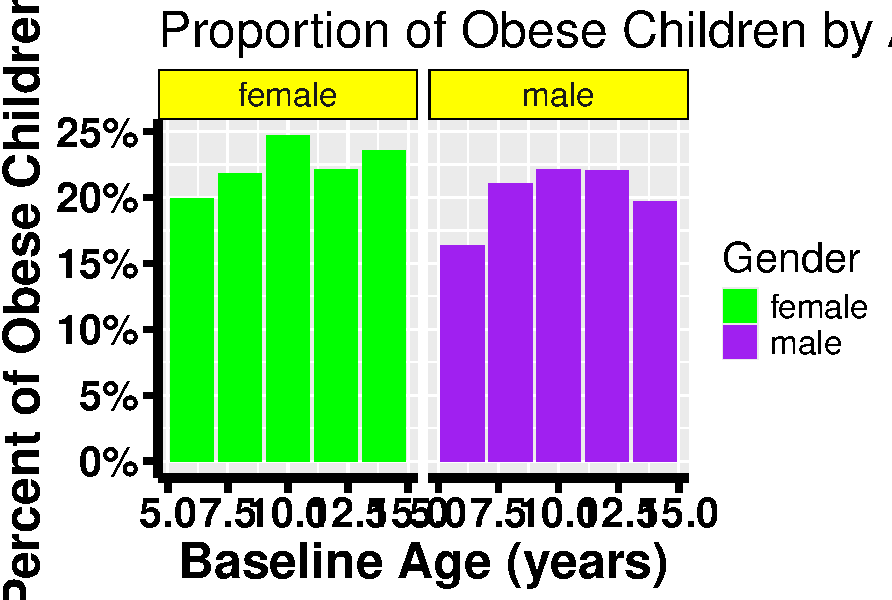
\includegraphics{Longi_noncontinuous_files/figure-pdf/unnamed-chunk-9-1.pdf}

}

\end{figure}

\begin{Shaded}
\begin{Highlighting}[]
\CommentTok{\# by subject, summarize the proportion of these T/F combinations}
\NormalTok{obesity\_prop\_by\_curr\_age }\OtherTok{\textless{}{-}}\NormalTok{ muscatine }\SpecialCharTok{\%\textgreater{}\%}
    \CommentTok{\# create a unique identifier for each combination (e.g. \textquotesingle{}TRUE{-}TRUE{-}FALSE\textquotesingle{})}
\FunctionTok{group\_by}\NormalTok{(curr\_age, gender\_label) }\SpecialCharTok{\%\textgreater{}\%}
    \CommentTok{\# prop of times each combo type occurs for a given subject:}
\FunctionTok{reframe}\NormalTok{(}\AttributeTok{prop =} \FunctionTok{mean}\NormalTok{(obesity\_status, }\AttributeTok{na.rm =}\NormalTok{ T), }\AttributeTok{times =} \FunctionTok{n}\NormalTok{())}
\end{Highlighting}
\end{Shaded}

Now that we have the proportions for each age group we create a new
variable.

\begin{Shaded}
\begin{Highlighting}[]
\NormalTok{lines }\OtherTok{\textless{}{-}} \FunctionTok{ggplot}\NormalTok{(obesity\_prop\_by\_curr\_age,}
                \FunctionTok{aes}\NormalTok{(}\AttributeTok{x =}\NormalTok{ curr\_age,}\AttributeTok{y =}\NormalTok{ prop,}\AttributeTok{color =}\NormalTok{ gender\_label)) }\SpecialCharTok{+} 
  \FunctionTok{geom\_line}\NormalTok{(}\AttributeTok{linewidth =} \DecValTok{3}\NormalTok{) }\SpecialCharTok{+}
  \FunctionTok{facet\_wrap}\NormalTok{(.}\SpecialCharTok{\textasciitilde{}}\NormalTok{gender\_label) }\SpecialCharTok{+} \CommentTok{\#this is what allows us to make separate boxes for the groups}
  \FunctionTok{theme}\NormalTok{(}\AttributeTok{axis.line =} \FunctionTok{element\_line}\NormalTok{(}\AttributeTok{colour =} \StringTok{"black"}\NormalTok{, }\AttributeTok{linewidth =} \DecValTok{2}\NormalTok{),}
        \AttributeTok{text =} \FunctionTok{element\_text}\NormalTok{(}\AttributeTok{size =} \DecValTok{20}\NormalTok{),}
        \AttributeTok{axis.text =} \FunctionTok{element\_text}\NormalTok{(}\AttributeTok{colour =} \StringTok{"black"}\NormalTok{, }\AttributeTok{size =} \DecValTok{20}\NormalTok{,}\AttributeTok{face =} \StringTok{"bold"}\NormalTok{),}
        \AttributeTok{axis.title =} \FunctionTok{element\_text}\NormalTok{(}\AttributeTok{size =} \DecValTok{24}\NormalTok{, }\AttributeTok{face =} \StringTok{"bold"}\NormalTok{),}
        \AttributeTok{axis.ticks.length =} \FunctionTok{unit}\NormalTok{(.}\DecValTok{25}\NormalTok{, }\StringTok{"cm"}\NormalTok{),}
        \AttributeTok{axis.ticks =} \FunctionTok{element\_line}\NormalTok{(}\AttributeTok{colour =} \StringTok{"black"}\NormalTok{, }\AttributeTok{linewidth =} \FloatTok{1.5}\NormalTok{),}
        \AttributeTok{strip.background=}\FunctionTok{element\_rect}\NormalTok{(}\AttributeTok{colour =} \StringTok{"black"}\NormalTok{, }\AttributeTok{fill =} \StringTok{"yellow"}\NormalTok{)) }\SpecialCharTok{+}
  \FunctionTok{scale\_fill\_manual}\NormalTok{(}\AttributeTok{name =} \StringTok{"Gender"}\NormalTok{,}\AttributeTok{values =} \FunctionTok{c}\NormalTok{(}\StringTok{"Female"} \OtherTok{=} \StringTok{"green"}\NormalTok{,}\StringTok{"Male"} \OtherTok{=} \StringTok{"purple"}\NormalTok{)) }\SpecialCharTok{+}
  \FunctionTok{scale\_y\_continuous}\NormalTok{(}\AttributeTok{labels =}\NormalTok{ percent) }\SpecialCharTok{+}
  \FunctionTok{ggtitle}\NormalTok{(}\StringTok{"Proportion of Obese Children by Age and Gender"}\NormalTok{) }\SpecialCharTok{+}
  \FunctionTok{ylab}\NormalTok{(}\StringTok{"Percent of Obese Children"}\NormalTok{) }\SpecialCharTok{+}
  \FunctionTok{xlab}\NormalTok{(}\StringTok{"Baseline Age (years)"}\NormalTok{)}

\NormalTok{lines}
\end{Highlighting}
\end{Shaded}

\begin{figure}[H]

{\centering 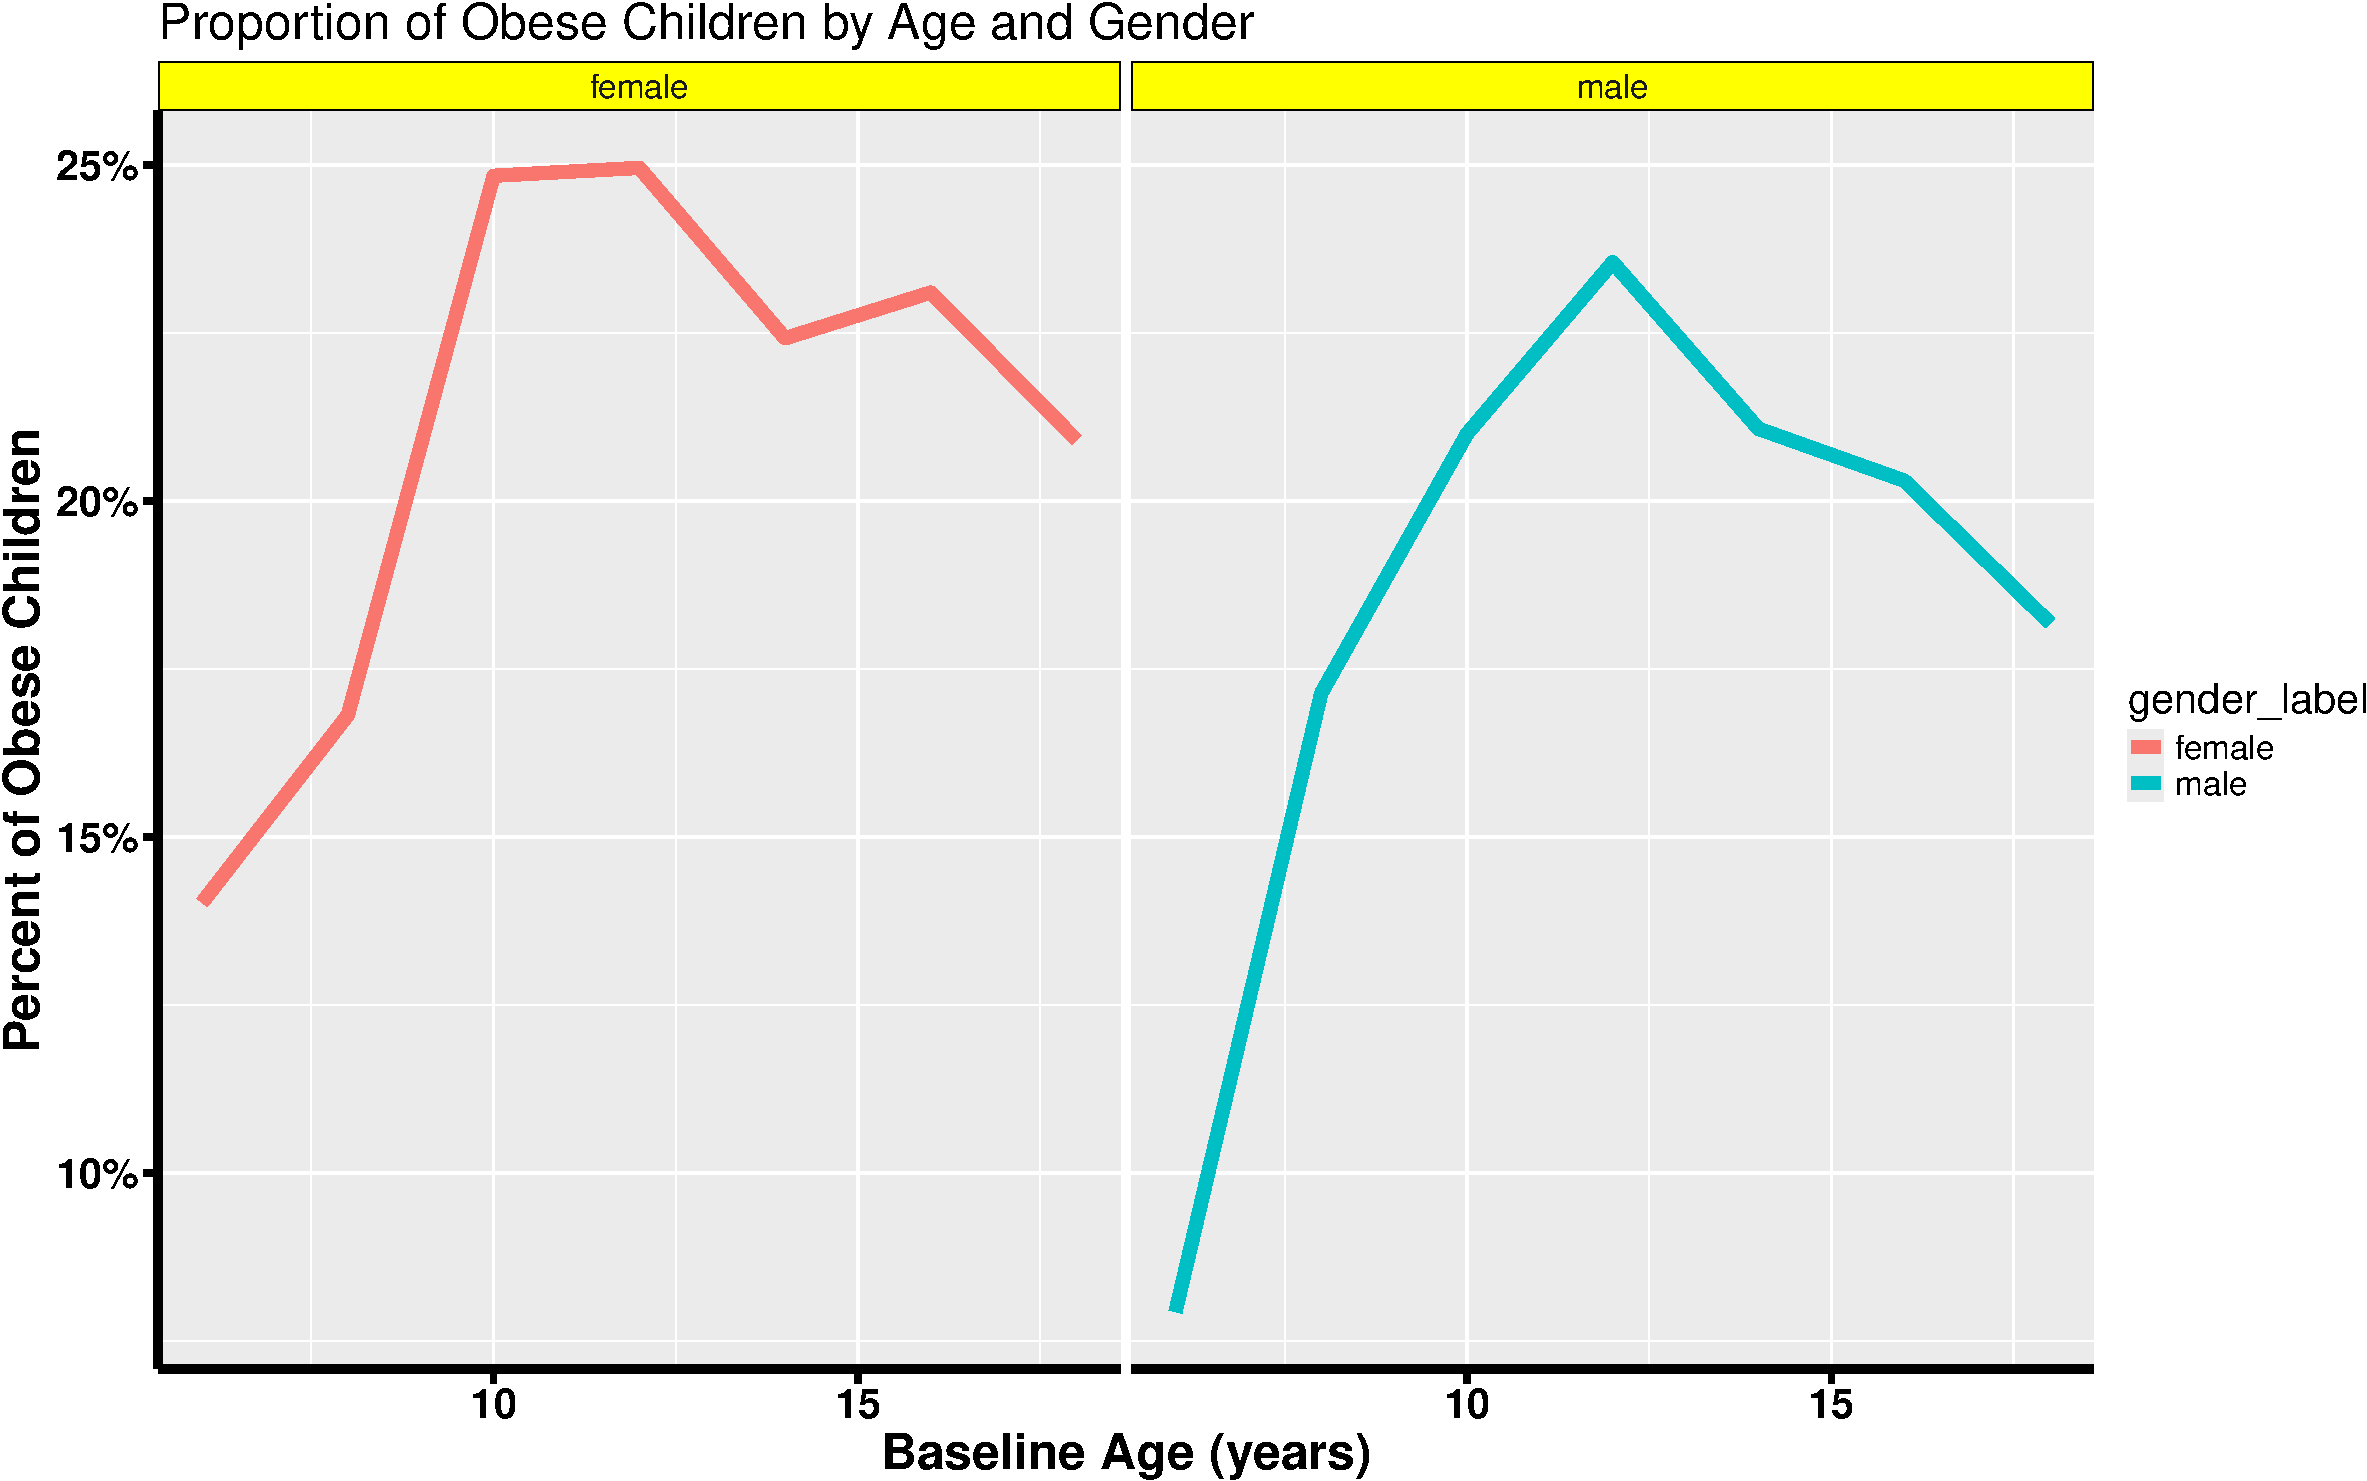
\includegraphics{Longi_noncontinuous_files/figure-pdf/unnamed-chunk-11-1.pdf}

}

\end{figure}

\hypertarget{marginal-models}{%
\section{Marginal Models}\label{marginal-models}}

\emph{Model 1:} This model includes gender, age, age\(^2\), and an
interaction term.

Model 1:
\(E(y_{ij} \mid X) = beta_{0} + \beta_{age}age + \beta_{age^2}age^2 + \beta_{gender}gender + \beta_{gender:age}gender*age + \beta_{gender:age^2}gender*age^2\).

\begin{Shaded}
\begin{Highlighting}[]
\NormalTok{model\_1 }\OtherTok{\textless{}{-}} \FunctionTok{geeglm}\NormalTok{(obesity\_status }\SpecialCharTok{\textasciitilde{}} \DecValTok{1} \SpecialCharTok{+}\NormalTok{ gender }\SpecialCharTok{+}\NormalTok{ centered\_age }\SpecialCharTok{+} \FunctionTok{I}\NormalTok{(centered\_age}\SpecialCharTok{\^{}}\DecValTok{2}\NormalTok{) }\SpecialCharTok{+}
\NormalTok{    centered\_age}\SpecialCharTok{:}\NormalTok{gender }\SpecialCharTok{+} \FunctionTok{I}\NormalTok{(centered\_age}\SpecialCharTok{\^{}}\DecValTok{2}\NormalTok{)}\SpecialCharTok{:}\NormalTok{gender, }\AttributeTok{id =}\NormalTok{ id, }\AttributeTok{data =}\NormalTok{ muscatine, }\AttributeTok{family =} \FunctionTok{binomial}\NormalTok{(}\AttributeTok{link =} \StringTok{"logit"}\NormalTok{),}
    \AttributeTok{corstr =} \StringTok{"unstructured"}\NormalTok{)}
\FunctionTok{summary}\NormalTok{(model\_1)}
\end{Highlighting}
\end{Shaded}

\begin{verbatim}

Call:
geeglm(formula = obesity_status ~ 1 + gender + centered_age + 
    I(centered_age^2) + centered_age:gender + I(centered_age^2):gender, 
    family = binomial(link = "logit"), data = muscatine, id = id, 
    corstr = "unstructured")

 Coefficients:
                          Estimate   Std.err    Wald Pr(>|W|)    
(Intercept)              -1.210629  0.050581 572.862  < 2e-16 ***
gender                    0.112872  0.071127   2.518  0.11253    
centered_age              0.040922  0.013348   9.398  0.00217 ** 
I(centered_age^2)        -0.017927  0.003388  28.002 1.21e-07 ***
gender:centered_age       0.005087  0.018349   0.077  0.78161    
gender:I(centered_age^2)  0.003883  0.004642   0.700  0.40295    
---
Signif. codes:  0 '***' 0.001 '**' 0.01 '*' 0.05 '.' 0.1 ' ' 1

Correlation structure = unstructured 
Estimated Scale Parameters:

            Estimate Std.err
(Intercept)   0.9925 0.02745
  Link = identity 

Estimated Correlation Parameters:
          Estimate Std.err
alpha.1:2   0.5792 0.02042
alpha.1:3   0.4624 0.03192
alpha.2:3   0.5589 0.03207
Number of clusters:   4856  Maximum cluster size: 3 
\end{verbatim}

\emph{Model 2:} This model includes gender, age, age\(^2\), and no
interaction term.

Model 2:
\(E(y_{ij} \mid X) = beta_{0} + \beta_{age}age + \beta_{age^2}age^2 + \beta_{gender}gender\).

\begin{Shaded}
\begin{Highlighting}[]
\NormalTok{model\_2 }\OtherTok{\textless{}{-}} \FunctionTok{geeglm}\NormalTok{(obesity\_status }\SpecialCharTok{\textasciitilde{}}\NormalTok{ gender }\SpecialCharTok{+}\NormalTok{ centered\_age }\SpecialCharTok{+} \FunctionTok{I}\NormalTok{(centered\_age}\SpecialCharTok{\^{}}\DecValTok{2}\NormalTok{), }\AttributeTok{id =}\NormalTok{ id,}
    \AttributeTok{data =}\NormalTok{ muscatine, }\AttributeTok{family =} \FunctionTok{binomial}\NormalTok{(}\AttributeTok{link =} \StringTok{"logit"}\NormalTok{), }\AttributeTok{corstr =} \StringTok{"unstructured"}\NormalTok{)}
\FunctionTok{summary}\NormalTok{(model\_2)}
\end{Highlighting}
\end{Shaded}

\begin{verbatim}

Call:
geeglm(formula = obesity_status ~ gender + centered_age + I(centered_age^2), 
    family = binomial(link = "logit"), data = muscatine, id = id, 
    corstr = "unstructured")

 Coefficients:
                  Estimate  Std.err  Wald Pr(>|W|)    
(Intercept)       -1.22520  0.04772 659.3  < 2e-16 ***
gender             0.14152  0.06270   5.1    0.024 *  
centered_age       0.04368  0.00915  22.8  1.8e-06 ***
I(centered_age^2) -0.01593  0.00231  47.4  5.8e-12 ***
---
Signif. codes:  0 '***' 0.001 '**' 0.01 '*' 0.05 '.' 0.1 ' ' 1

Correlation structure = unstructured 
Estimated Scale Parameters:

            Estimate Std.err
(Intercept)    0.992  0.0274
  Link = identity 

Estimated Correlation Parameters:
          Estimate Std.err
alpha.1:2    0.580  0.0204
alpha.1:3    0.462  0.0319
alpha.2:3    0.558  0.0320
Number of clusters:   4856  Maximum cluster size: 3 
\end{verbatim}

Now that we have our two models what do we do with them? As mentioned
before the purpose is to predict probabilities so let's do just that.
This can be done through the predict() function. To return predicted
probabilities specify type as ``response''. To get back the linear
predictions (i.e.~the natural log of the odds ratio
\(\frac{P(Y=1| \mid X)}{1-P(Y=1 \mid X)}\) in this case) specify type as
``link'' (i.e.~for link function). A third option is to specify type as
``terms''. This gives you back an \(N \times (p-1)\) matrix where each
column corresponds to the product of the estimated coefficient
\(\beta_j\) and the corresponding covariate \(X_j\). This is not done
for the intercept so that must be done manually.

\begin{Shaded}
\begin{Highlighting}[]
\CommentTok{\# calculate predicted probabilities for model 1}
\NormalTok{model\_1\_probs }\OtherTok{\textless{}{-}} \FunctionTok{predict}\NormalTok{(model\_1, }\AttributeTok{type =} \StringTok{"response"}\NormalTok{)}

\CommentTok{\# calculate predicted probabilities for model 2}
\NormalTok{model\_2\_probs }\OtherTok{\textless{}{-}} \FunctionTok{predict}\NormalTok{(model\_2, }\AttributeTok{type =} \StringTok{"response"}\NormalTok{)}
\end{Highlighting}
\end{Shaded}

Now that we have these two probability vectors what do we do with them?
We can see how these probabilities vary with respect to age and gender.

We can create plots. We will take the predicted probabilities and plot
them against the observed. To do so we begin by taking the mean
predicted probability within each Age/Gender strata. To make that
clearer, for example we look at the predicted probabilities for all 14
year old males and find their mean.

Note: Uncomment this after you defined model\_2\_probs

\begin{Shaded}
\begin{Highlighting}[]
\CommentTok{\#create new dataset that removes missing values}
\NormalTok{muscatine\_complete }\OtherTok{\textless{}{-}} \FunctionTok{na.omit}\NormalTok{(muscatine)}

\CommentTok{\# add in probabilities as covariates}
\NormalTok{muscatine\_complete[,model\_1 }\SpecialCharTok{:}\ErrorTok{=}\NormalTok{ model\_1\_probs]}
\NormalTok{muscatine\_complete[,model\_2 }\SpecialCharTok{:}\ErrorTok{=}\NormalTok{ model\_2\_probs]}

\CommentTok{\# by subject, summarize the proportion of these T/F combinations }
\NormalTok{gee\_probs }\OtherTok{\textless{}{-}} \FunctionTok{data.table}\NormalTok{(muscatine\_complete }\SpecialCharTok{\%\textgreater{}\%}
  \CommentTok{\# create a unique identifier for each combination (e.g. "TRUE{-}TRUE{-}FALSE")}
  \FunctionTok{group\_by}\NormalTok{(curr\_age, gender\_label) }\SpecialCharTok{\%\textgreater{}\%}
  \CommentTok{\# prop of times each combo type occurs for a given subject:}
  \FunctionTok{reframe}\NormalTok{(}\AttributeTok{prop =} \FunctionTok{mean}\NormalTok{(obesity\_status, }\AttributeTok{na.rm =}\NormalTok{ T),}
          \AttributeTok{prob\_1 =} \FunctionTok{mean}\NormalTok{(model\_1),}
          \AttributeTok{prob\_2 =} \FunctionTok{mean}\NormalTok{(model\_2)))}

\NormalTok{df\_models }\OtherTok{\textless{}{-}} \FunctionTok{data.frame}\NormalTok{(}\StringTok{"Age"} \OtherTok{=} \FunctionTok{unique}\NormalTok{(gee\_probs[, curr\_age]),}
                    \StringTok{"Est\_Female1"} \OtherTok{=}\NormalTok{ gee\_probs[gender\_label }\SpecialCharTok{==} \StringTok{"female"}\NormalTok{, prob\_1],}
                    \StringTok{"Est\_Male1"} \OtherTok{=}\NormalTok{ gee\_probs[gender\_label }\SpecialCharTok{==} \StringTok{"male"}\NormalTok{, prob\_1],}
                    \StringTok{"Est\_Female2"} \OtherTok{=}\NormalTok{ gee\_probs[gender\_label }\SpecialCharTok{==} \StringTok{"female"}\NormalTok{, prob\_2],}
                    \StringTok{"Est\_Male2"} \OtherTok{=}\NormalTok{ gee\_probs[gender\_label }\SpecialCharTok{==} \StringTok{"male"}\NormalTok{, prob\_2],}
                     \StringTok{"Obs\_Female"} \OtherTok{=}\NormalTok{ gee\_probs[gender\_label }\SpecialCharTok{==} \StringTok{"female"}\NormalTok{, prop],}
                     \StringTok{"Obs\_Male"} \OtherTok{=}\NormalTok{ gee\_probs[gender\_label }\SpecialCharTok{==} \StringTok{"male"}\NormalTok{, prop])}
\end{Highlighting}
\end{Shaded}

\begin{Shaded}
\begin{Highlighting}[]
\NormalTok{labels }\OtherTok{\textless{}{-}} \FunctionTok{c}\NormalTok{(}\StringTok{"Est. Probability, Female"}\NormalTok{, }\StringTok{"Est. Probability, Male"}\NormalTok{, }\StringTok{"Obs. Proportion, Female"}\NormalTok{,}
    \StringTok{"Obs. Proportion, Male"}\NormalTok{)}
\NormalTok{df }\OtherTok{\textless{}{-}} \FunctionTok{data.frame}\NormalTok{(}\AttributeTok{x =} \FunctionTok{rep}\NormalTok{(df\_models[, }\StringTok{"Age"}\NormalTok{], }\AttributeTok{times =} \DecValTok{4}\NormalTok{), }\AttributeTok{y =} \FunctionTok{c}\NormalTok{(df\_models[, }\StringTok{"Est\_Female1"}\NormalTok{],}
\NormalTok{    df\_models[, }\StringTok{"Est\_Male1"}\NormalTok{], df\_models[, }\StringTok{"Obs\_Female"}\NormalTok{], df\_models[, }\StringTok{"Obs\_Male"}\NormalTok{]),}
    \AttributeTok{group =} \FunctionTok{rep}\NormalTok{(labels, }\AttributeTok{each =} \DecValTok{7}\NormalTok{))}

\NormalTok{df }\SpecialCharTok{\%\textgreater{}\%}
    \FunctionTok{ggplot}\NormalTok{() }\SpecialCharTok{+} \FunctionTok{geom\_line}\NormalTok{(}\FunctionTok{aes}\NormalTok{(x, y, }\AttributeTok{color =}\NormalTok{ group, }\AttributeTok{linetype =}\NormalTok{ group), }\AttributeTok{linewidth =} \DecValTok{2}\NormalTok{) }\SpecialCharTok{+}
    \FunctionTok{theme}\NormalTok{(}\AttributeTok{axis.line =} \FunctionTok{element\_line}\NormalTok{(}\AttributeTok{colour =} \StringTok{"black"}\NormalTok{, }\AttributeTok{linewidth =} \DecValTok{2}\NormalTok{), }\AttributeTok{text =} \FunctionTok{element\_text}\NormalTok{(}\AttributeTok{size =} \DecValTok{20}\NormalTok{),}
        \AttributeTok{axis.text =} \FunctionTok{element\_text}\NormalTok{(}\AttributeTok{colour =} \StringTok{"black"}\NormalTok{, }\AttributeTok{size =} \DecValTok{20}\NormalTok{, }\AttributeTok{face =} \StringTok{"bold"}\NormalTok{), }\AttributeTok{axis.title =} \FunctionTok{element\_text}\NormalTok{(}\AttributeTok{size =} \DecValTok{24}\NormalTok{,}
            \AttributeTok{face =} \StringTok{"bold"}\NormalTok{), }\AttributeTok{axis.ticks.length =} \FunctionTok{unit}\NormalTok{(}\FloatTok{0.25}\NormalTok{, }\StringTok{"cm"}\NormalTok{), }\AttributeTok{axis.ticks =} \FunctionTok{element\_line}\NormalTok{(}\AttributeTok{colour =} \StringTok{"black"}\NormalTok{,}
            \AttributeTok{linewidth =} \FloatTok{1.5}\NormalTok{)) }\SpecialCharTok{+} \FunctionTok{scale\_color\_manual}\NormalTok{(}\AttributeTok{name =} \StringTok{""}\NormalTok{, }\AttributeTok{labels =}\NormalTok{ labels, }\AttributeTok{values =} \FunctionTok{c}\NormalTok{(}\StringTok{"darkred"}\NormalTok{,}
    \StringTok{"darkblue"}\NormalTok{, }\StringTok{"red"}\NormalTok{, }\StringTok{"dodgerblue3"}\NormalTok{)) }\SpecialCharTok{+} \FunctionTok{scale\_linetype\_manual}\NormalTok{(}\AttributeTok{name =} \StringTok{""}\NormalTok{, }\AttributeTok{labels =}\NormalTok{ labels,}
    \AttributeTok{values =} \FunctionTok{c}\NormalTok{(}\StringTok{"dashed"}\NormalTok{, }\StringTok{"dashed"}\NormalTok{, }\StringTok{"solid"}\NormalTok{, }\StringTok{"solid"}\NormalTok{)) }\SpecialCharTok{+} \FunctionTok{scale\_y\_continuous}\NormalTok{(}\AttributeTok{labels =}\NormalTok{ percent) }\SpecialCharTok{+}
    \FunctionTok{ggtitle}\NormalTok{(}\StringTok{"Marginal Model 1: Observed vs Predicted Probabilities"}\NormalTok{) }\SpecialCharTok{+} \FunctionTok{ylab}\NormalTok{(}\StringTok{"Percent of Obese Children"}\NormalTok{) }\SpecialCharTok{+}
    \FunctionTok{xlab}\NormalTok{(}\StringTok{"Age (years)"}\NormalTok{)}
\end{Highlighting}
\end{Shaded}

\begin{figure}[H]

{\centering 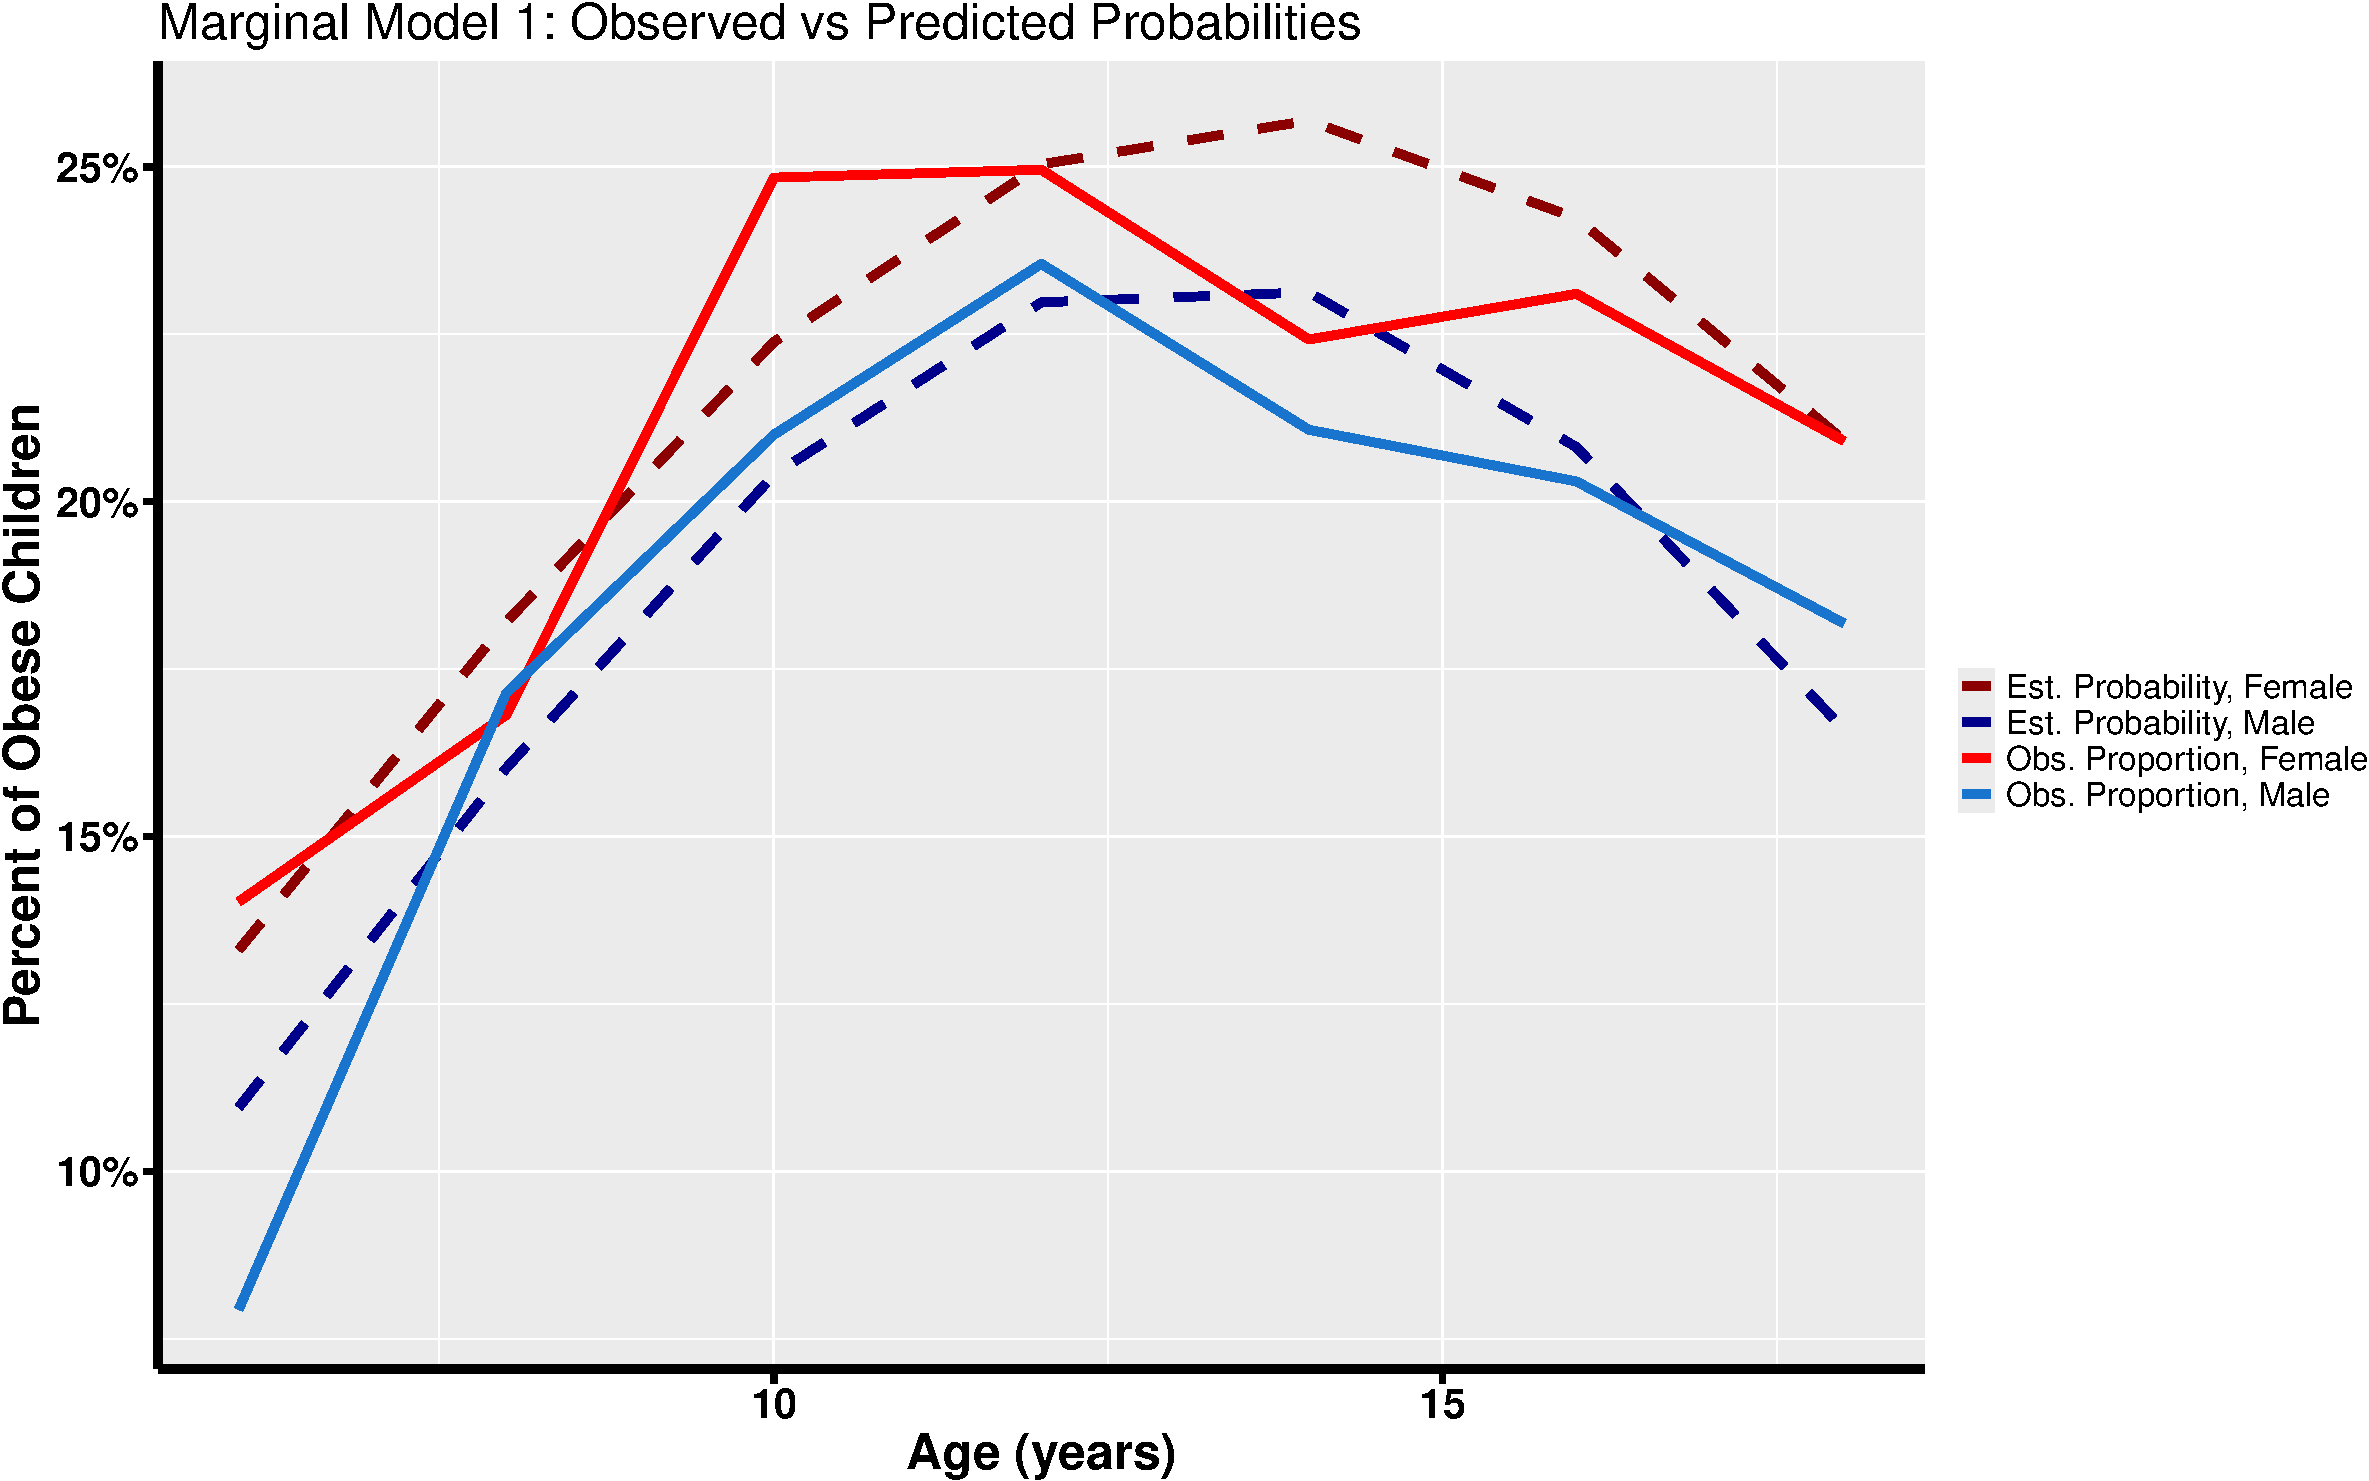
\includegraphics{Longi_noncontinuous_files/figure-pdf/unnamed-chunk-16-1.pdf}

}

\end{figure}

\begin{Shaded}
\begin{Highlighting}[]
\NormalTok{df }\OtherTok{\textless{}{-}} \FunctionTok{data.frame}\NormalTok{(}\AttributeTok{x =} \FunctionTok{rep}\NormalTok{(df\_models[, }\StringTok{"Age"}\NormalTok{], }\AttributeTok{times =} \DecValTok{4}\NormalTok{), }\AttributeTok{y =} \FunctionTok{c}\NormalTok{(df\_models[, }\StringTok{"Est\_Female2"}\NormalTok{],}
\NormalTok{    df\_models[, }\StringTok{"Est\_Male2"}\NormalTok{], df\_models[, }\StringTok{"Obs\_Female"}\NormalTok{], df\_models[, }\StringTok{"Obs\_Male"}\NormalTok{]),}
    \AttributeTok{group =} \FunctionTok{rep}\NormalTok{(labels, }\AttributeTok{each =} \DecValTok{7}\NormalTok{))}

\NormalTok{df }\SpecialCharTok{\%\textgreater{}\%}
    \FunctionTok{ggplot}\NormalTok{() }\SpecialCharTok{+} \FunctionTok{geom\_line}\NormalTok{(}\FunctionTok{aes}\NormalTok{(x, y, }\AttributeTok{color =}\NormalTok{ group, }\AttributeTok{linetype =}\NormalTok{ group), }\AttributeTok{linewidth =} \DecValTok{2}\NormalTok{) }\SpecialCharTok{+}
    \FunctionTok{theme}\NormalTok{(}\AttributeTok{axis.line =} \FunctionTok{element\_line}\NormalTok{(}\AttributeTok{colour =} \StringTok{"black"}\NormalTok{, }\AttributeTok{linewidth =} \DecValTok{2}\NormalTok{), }\AttributeTok{text =} \FunctionTok{element\_text}\NormalTok{(}\AttributeTok{size =} \DecValTok{20}\NormalTok{),}
        \AttributeTok{axis.text =} \FunctionTok{element\_text}\NormalTok{(}\AttributeTok{colour =} \StringTok{"black"}\NormalTok{, }\AttributeTok{size =} \DecValTok{20}\NormalTok{, }\AttributeTok{face =} \StringTok{"bold"}\NormalTok{), }\AttributeTok{axis.title =} \FunctionTok{element\_text}\NormalTok{(}\AttributeTok{size =} \DecValTok{24}\NormalTok{,}
            \AttributeTok{face =} \StringTok{"bold"}\NormalTok{), }\AttributeTok{axis.ticks.length =} \FunctionTok{unit}\NormalTok{(}\FloatTok{0.25}\NormalTok{, }\StringTok{"cm"}\NormalTok{), }\AttributeTok{axis.ticks =} \FunctionTok{element\_line}\NormalTok{(}\AttributeTok{colour =} \StringTok{"black"}\NormalTok{,}
            \AttributeTok{linewidth =} \FloatTok{1.5}\NormalTok{)) }\SpecialCharTok{+} \FunctionTok{scale\_color\_manual}\NormalTok{(}\AttributeTok{name =} \StringTok{" "}\NormalTok{, }\AttributeTok{labels =}\NormalTok{ labels, }\AttributeTok{values =} \FunctionTok{c}\NormalTok{(}\StringTok{"darkred"}\NormalTok{,}
    \StringTok{"darkblue"}\NormalTok{, }\StringTok{"red"}\NormalTok{, }\StringTok{"dodgerblue3"}\NormalTok{)) }\SpecialCharTok{+} \FunctionTok{scale\_linetype\_manual}\NormalTok{(}\AttributeTok{name =} \StringTok{" "}\NormalTok{, }\AttributeTok{labels =}\NormalTok{ labels,}
    \AttributeTok{values =} \FunctionTok{c}\NormalTok{(}\StringTok{"dashed"}\NormalTok{, }\StringTok{"dashed"}\NormalTok{, }\StringTok{"solid"}\NormalTok{, }\StringTok{"solid"}\NormalTok{)) }\SpecialCharTok{+} \FunctionTok{scale\_y\_continuous}\NormalTok{(}\AttributeTok{labels =}\NormalTok{ percent) }\SpecialCharTok{+}
    \FunctionTok{ggtitle}\NormalTok{(}\StringTok{"Marginal Model 2: Observed vs Predicted Probabilities"}\NormalTok{) }\SpecialCharTok{+} \FunctionTok{ylab}\NormalTok{(}\StringTok{"Percent of Obese Children"}\NormalTok{) }\SpecialCharTok{+}
    \FunctionTok{xlab}\NormalTok{(}\StringTok{"Age (years)"}\NormalTok{)}
\end{Highlighting}
\end{Shaded}

\begin{figure}[H]

{\centering 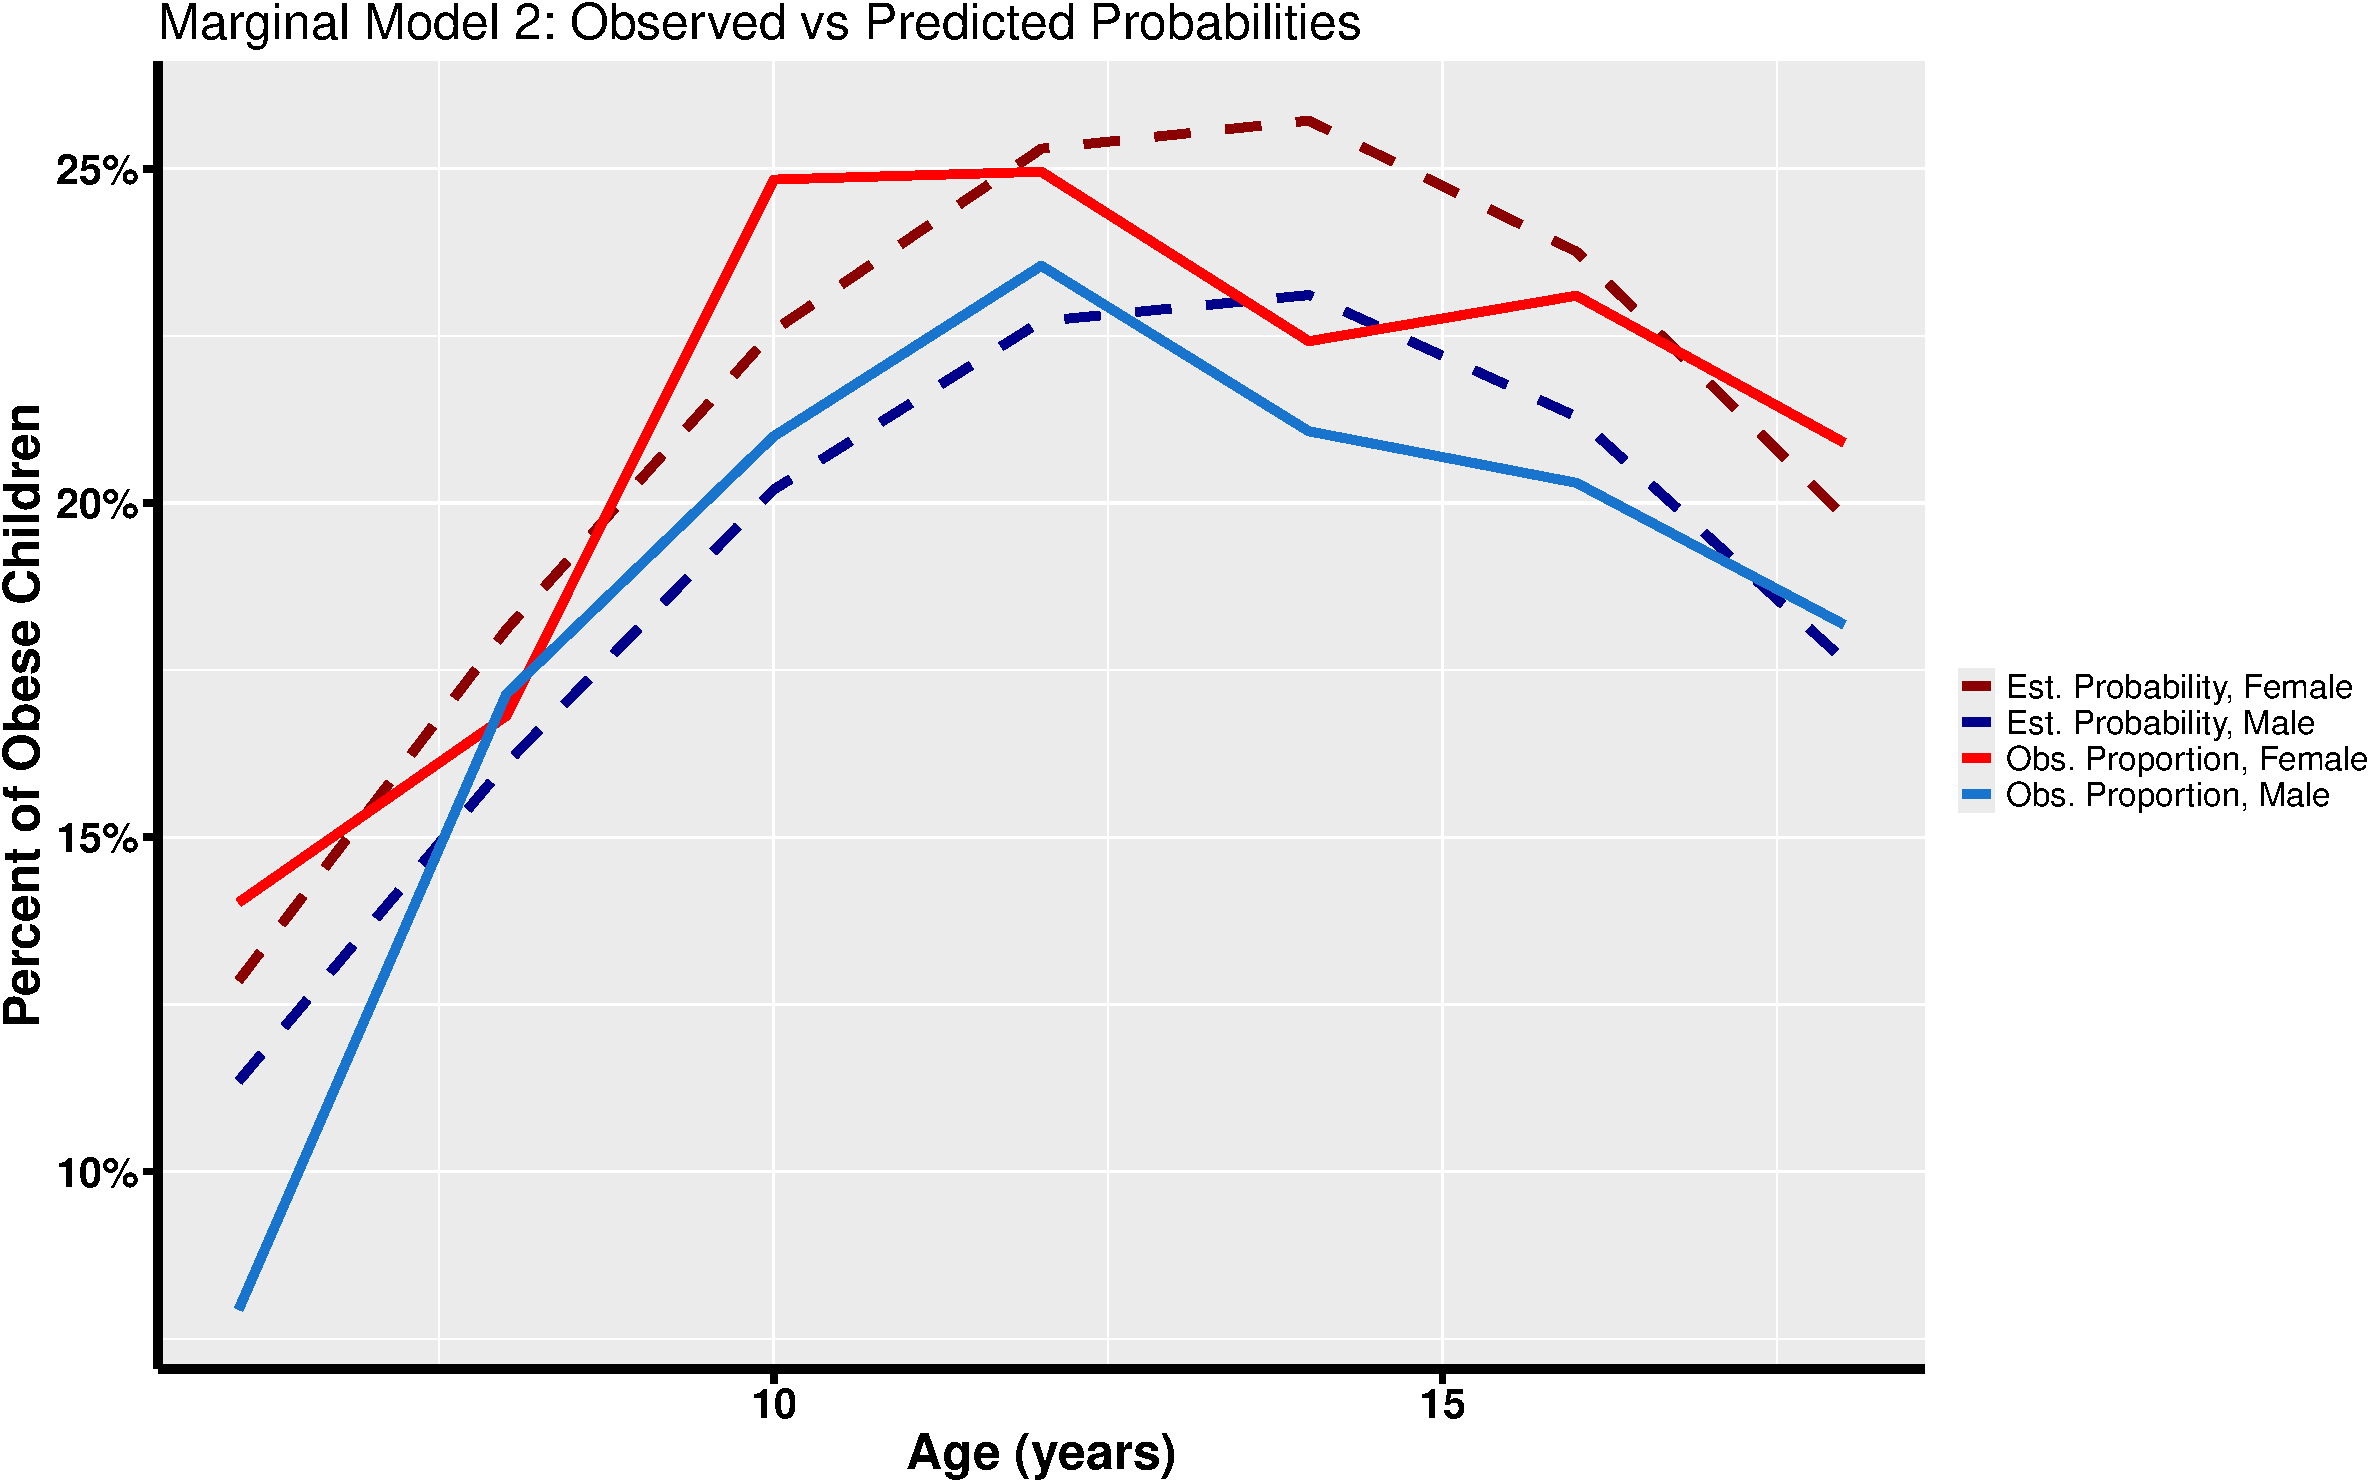
\includegraphics{Longi_noncontinuous_files/figure-pdf/unnamed-chunk-17-1.pdf}

}

\end{figure}

\hypertarget{mixed-effect-models}{%
\section{Mixed Effect Models}\label{mixed-effect-models}}

In this section we will fit Mixed-Effects (subject-specific) Models for
longitudinal data, when the outcome of interest is a non-continuous
variable.

Recall that a Generalized Mixed Effects Model has the following form:
\(g(E[y_{ij} \mid X] )= X_{i}\beta + Z_{i}b_i\). Here
\(g(p) = logit(p)\).

\emph{Model 3:} We fit a mixed-effects model with gender, age,
age\(^2\), and an interaction term, and a random intercept.

Model 3:
\(logit(E[y_{i} \mid b_i, X_i, \beta])= beta_{0} + \beta_{age}age + \beta_{age^2}age^2 + \beta_{gender}gender + \beta_{gender:age}gender*age + \beta_{gender:age^2}gender*age^2 + b_{0,i}\).

The (1\textbar id) means that we are allowing the intercept, represented
by 1, to vary by patient.

\begin{Shaded}
\begin{Highlighting}[]
\NormalTok{model\_3 }\OtherTok{\textless{}{-}} \FunctionTok{glmer}\NormalTok{(obesity\_status }\SpecialCharTok{\textasciitilde{}} \DecValTok{1} \SpecialCharTok{+}\NormalTok{ gender }\SpecialCharTok{+}\NormalTok{ centered\_age }\SpecialCharTok{+} \FunctionTok{I}\NormalTok{(centered\_age}\SpecialCharTok{\^{}}\DecValTok{2}\NormalTok{) }\SpecialCharTok{+}
\NormalTok{    centered\_age}\SpecialCharTok{:}\NormalTok{gender }\SpecialCharTok{+} \FunctionTok{I}\NormalTok{(centered\_age}\SpecialCharTok{\^{}}\DecValTok{2}\NormalTok{)}\SpecialCharTok{:}\NormalTok{gender }\SpecialCharTok{+}\NormalTok{ (}\DecValTok{1} \SpecialCharTok{|}\NormalTok{ id), }\AttributeTok{family =} \FunctionTok{binomial}\NormalTok{(}\AttributeTok{link =} \StringTok{"logit"}\NormalTok{),}
    \AttributeTok{data =}\NormalTok{ muscatine, }\AttributeTok{nAGQ =} \DecValTok{7}\NormalTok{)}
\FunctionTok{summary}\NormalTok{(model\_3)}
\end{Highlighting}
\end{Shaded}

\begin{verbatim}
Generalized linear mixed model fit by maximum likelihood (Adaptive
  Gauss-Hermite Quadrature, nAGQ = 7) [glmerMod]
 Family: binomial  ( logit )
Formula: obesity_status ~ 1 + gender + centered_age + I(centered_age^2) +  
    centered_age:gender + I(centered_age^2):gender + (1 | id)
   Data: muscatine

     AIC      BIC   logLik deviance df.resid 
    8729     8780    -4358     8715     9849 

Scaled residuals: 
   Min     1Q Median     3Q    Max 
-1.546 -0.192 -0.174 -0.115  2.522 

Random effects:
 Groups Name        Variance Std.Dev.
 id     (Intercept) 9.91     3.15    
Number of obs: 9856, groups:  id, 4856

Fixed effects:
                         Estimate Std. Error z value Pr(>|z|)    
(Intercept)              -2.70752    0.12460  -21.73  < 2e-16 ***
gender                    0.25269    0.15136    1.67   0.0950 .  
centered_age              0.08330    0.02710    3.07   0.0021 ** 
I(centered_age^2)        -0.03785    0.00688   -5.50  3.7e-08 ***
gender:centered_age       0.01719    0.03795    0.45   0.6506    
gender:I(centered_age^2)  0.00807    0.00959    0.84   0.3998    
---
Signif. codes:  0 '***' 0.001 '**' 0.01 '*' 0.05 '.' 0.1 ' ' 1

Correlation of Fixed Effects:
            (Intr) gender cntrd_ I(_^2) gndr:_
gender      -0.635                            
centered_ag -0.033 -0.008                     
I(cntrd_^2) -0.349  0.336 -0.041              
gndr:cntrd_ -0.024  0.013 -0.705  0.017       
gndr:I(_^2)  0.286 -0.486  0.023 -0.708 -0.043
\end{verbatim}

One thing you might notice about the \texttt{glmer()} function and its
output are integration points and the parameter \texttt{nAGQ}, which
specifies said points. When the distribution we're dealing with isn't
normal and the link function \(g()\) isn't the identity we can't derive
an analytic solution.

In fact the log likelihood \(\ell(\beta)\) looks like:
\(\ell(\beta) = \sum^N_{i=1}log( p(y_j \mid \beta) ) = \sum^N_{i=1}log( \int p(y_j \mid b_j,X_j, \beta)p(b_j \mid \beta) db_j)\)

The integral in the definition does not have a closed-form solution, and
numerical approximations are required to obtain the maximum likelihood
estimates. So when you see the word Adaptive Gauss-Hermite Quadrature
that is simply the method that we use to approximate the integral.

For those who are curious, Gauss-Hermite Quadrature is a method for
approximating integrals of the following form:
\(\int e^{-x^2} f(x)dx \approx \sum^K_{k=1}w_k f(x_k)\) where we pick k
points (i.e.~the integration points). The \(x_k\) are the roots of the
\(K^{th}\) order Hermite polynomial \(H_K(x)\) where
\(H_K(x) = (-1)^K e^{x^2} \frac{d^K}{dx^K}e^{-x^2}\), and
\(w_k = \frac{2^{K-1}K!\sqrt{\pi}}{K^2[H_{K-1}(x_k)]^2}\). Adaptive
Gauss Qudrature chooses the integration points \(x_k\) through a
different method, but the specification of the weights \(w_k\) remains
the same.

For \(K=1\) this is just the Laplace Approximation method for
integration which \texttt{glmer()} uses automatically. If you want to
use Adaptive Gauss Hermite you need to specify \texttt{nAGQ}
\textgreater{} 1. I mention this because STATA uses adaptive and
non-adaptive Gauss Hermite Quadrature to estimate the integral.

\emph{Model 4:} We fit a mixed-effects model with gender, age,
age\(^2\), with no interaction term, and a random intercept.

Model 4:
\(logit(E[y_{i} \mid b_i, X_i, \beta]) = beta_{0} + \beta_{age}age + \beta_{age^2}age^2 + b_{0,i}\).

\begin{Shaded}
\begin{Highlighting}[]
\CommentTok{\# name this model \textquotesingle{}model\_4\textquotesingle{}}

\NormalTok{model\_4 }\OtherTok{\textless{}{-}} \FunctionTok{glmer}\NormalTok{(obesity\_status }\SpecialCharTok{\textasciitilde{}} \DecValTok{1} \SpecialCharTok{+}\NormalTok{ gender }\SpecialCharTok{+}\NormalTok{ centered\_age }\SpecialCharTok{+} \FunctionTok{I}\NormalTok{(centered\_age}\SpecialCharTok{\^{}}\DecValTok{2}\NormalTok{) }\SpecialCharTok{+}
\NormalTok{    (}\DecValTok{1} \SpecialCharTok{|}\NormalTok{ id), }\AttributeTok{data =}\NormalTok{ muscatine, }\AttributeTok{family =} \FunctionTok{binomial}\NormalTok{(}\AttributeTok{link =} \StringTok{"logit"}\NormalTok{), }\AttributeTok{nAGQ =} \DecValTok{7}\NormalTok{)}
\FunctionTok{summary}\NormalTok{(model\_4)}
\end{Highlighting}
\end{Shaded}

\begin{verbatim}
Generalized linear mixed model fit by maximum likelihood (Adaptive
  Gauss-Hermite Quadrature, nAGQ = 7) [glmerMod]
 Family: binomial  ( logit )
Formula: obesity_status ~ 1 + gender + centered_age + I(centered_age^2) +  
    (1 | id)
   Data: muscatine

     AIC      BIC   logLik deviance df.resid 
    8726     8762    -4358     8716     9851 

Scaled residuals: 
   Min     1Q Median     3Q    Max 
-1.545 -0.193 -0.170 -0.116  2.602 

Random effects:
 Groups Name        Variance Std.Dev.
 id     (Intercept) 9.9      3.15    
Number of obs: 9856, groups:  id, 4856

Fixed effects:
                  Estimate Std. Error z value Pr(>|z|)    
(Intercept)       -2.73777    0.11945  -22.92  < 2e-16 ***
gender             0.31539    0.13215    2.39    0.017 *  
centered_age       0.09211    0.01921    4.80  1.6e-06 ***
I(centered_age^2) -0.03375    0.00485   -6.96  3.5e-12 ***
---
Signif. codes:  0 '***' 0.001 '**' 0.01 '*' 0.05 '.' 0.1 ' ' 1

Correlation of Fixed Effects:
            (Intr) gender cntrd_
gender      -0.594              
centered_ag -0.072 -0.001       
I(cntrd_^2) -0.219 -0.010 -0.068
\end{verbatim}

\begin{Shaded}
\begin{Highlighting}[]
\CommentTok{\# calculate predicted probabilities for model 3}
\NormalTok{model\_3\_probs }\OtherTok{\textless{}{-}} \FunctionTok{predict}\NormalTok{(model\_3, }\AttributeTok{type =} \StringTok{"response"}\NormalTok{)}

\CommentTok{\# calculate predicted probabilities for model 4}
\NormalTok{model\_4\_probs }\OtherTok{\textless{}{-}} \FunctionTok{predict}\NormalTok{(model\_4, }\AttributeTok{type =} \StringTok{"response"}\NormalTok{)}
\end{Highlighting}
\end{Shaded}

Note: Uncomment this after you define model\_3\_probs and
model\_4\_probs

\begin{Shaded}
\begin{Highlighting}[]
\CommentTok{\# add in probabilities as covariates}
\NormalTok{muscatine\_complete[, model\_3 }\SpecialCharTok{:}\ErrorTok{=}\NormalTok{ model\_3\_probs]}
\NormalTok{muscatine\_complete[, model\_4 }\SpecialCharTok{:}\ErrorTok{=}\NormalTok{ model\_4\_probs]}
\end{Highlighting}
\end{Shaded}

\begin{Shaded}
\begin{Highlighting}[]
\CommentTok{\# by subject, summarize the proportion of these T/F combinations }
\NormalTok{mem\_probs }\OtherTok{\textless{}{-}} \FunctionTok{data.table}\NormalTok{( muscatine\_complete }\SpecialCharTok{\%\textgreater{}\%}
  \CommentTok{\# create a unique identifier for each combination (e.g. "TRUE{-}TRUE{-}FALSE")}
  \FunctionTok{group\_by}\NormalTok{(curr\_age, gender\_label) }\SpecialCharTok{\%\textgreater{}\%}
  \CommentTok{\# prop of times each combo type occurs for a given subject:}
  \FunctionTok{reframe}\NormalTok{(}\AttributeTok{prob\_3 =} \FunctionTok{max}\NormalTok{(model\_3),}
          \AttributeTok{prob\_4 =} \FunctionTok{max}\NormalTok{(model\_4)))}
\NormalTok{df\_models2 }\OtherTok{\textless{}{-}} \FunctionTok{cbind}\NormalTok{(df\_models, }\FunctionTok{data.frame}\NormalTok{(}\StringTok{"Est\_Female3"} \OtherTok{=}\NormalTok{ mem\_probs[gender\_label }\SpecialCharTok{==} \StringTok{"female"}\NormalTok{, prob\_3],}
                                          \StringTok{"Est\_Male3"} \OtherTok{=}\NormalTok{ mem\_probs[gender\_label }\SpecialCharTok{==} \StringTok{"male"}\NormalTok{, prob\_3],}
                                          \StringTok{"Est\_Female4"} \OtherTok{=}\NormalTok{ mem\_probs[gender\_label }\SpecialCharTok{==} \StringTok{"female"}\NormalTok{, prob\_4],}
                                          \StringTok{"Est\_Male4"} \OtherTok{=}\NormalTok{ mem\_probs[gender\_label }\SpecialCharTok{==} \StringTok{"male"}\NormalTok{, prob\_4]))}
\NormalTok{df\_models2 }\OtherTok{\textless{}{-}} \FunctionTok{as.data.frame}\NormalTok{(df\_models2)}
\end{Highlighting}
\end{Shaded}

\begin{Shaded}
\begin{Highlighting}[]
\NormalTok{df }\OtherTok{\textless{}{-}} \FunctionTok{data.frame}\NormalTok{(}\AttributeTok{x =} \FunctionTok{rep}\NormalTok{(df\_models[, }\StringTok{"Age"}\NormalTok{], }\AttributeTok{times =} \DecValTok{4}\NormalTok{), }\AttributeTok{y =} \FunctionTok{c}\NormalTok{(df\_models2[, }\StringTok{"Est\_Female3"}\NormalTok{],}
\NormalTok{    df\_models2[, }\StringTok{"Est\_Male3"}\NormalTok{], df\_models2[, }\StringTok{"Obs\_Female"}\NormalTok{], df\_models2[, }\StringTok{"Obs\_Male"}\NormalTok{]),}
    \AttributeTok{group =} \FunctionTok{rep}\NormalTok{(labels, }\AttributeTok{each =} \DecValTok{7}\NormalTok{))}

\NormalTok{df }\SpecialCharTok{\%\textgreater{}\%}
    \FunctionTok{ggplot}\NormalTok{() }\SpecialCharTok{+} \FunctionTok{geom\_line}\NormalTok{(}\FunctionTok{aes}\NormalTok{(x, y, }\AttributeTok{color =}\NormalTok{ group, }\AttributeTok{linetype =}\NormalTok{ group), }\AttributeTok{linewidth =} \DecValTok{2}\NormalTok{) }\SpecialCharTok{+}
    \FunctionTok{theme}\NormalTok{(}\AttributeTok{axis.line =} \FunctionTok{element\_line}\NormalTok{(}\AttributeTok{colour =} \StringTok{"black"}\NormalTok{, }\AttributeTok{linewidth =} \DecValTok{2}\NormalTok{), }\AttributeTok{text =} \FunctionTok{element\_text}\NormalTok{(}\AttributeTok{size =} \DecValTok{20}\NormalTok{),}
        \AttributeTok{axis.text =} \FunctionTok{element\_text}\NormalTok{(}\AttributeTok{colour =} \StringTok{"black"}\NormalTok{, }\AttributeTok{size =} \DecValTok{20}\NormalTok{, }\AttributeTok{face =} \StringTok{"bold"}\NormalTok{), }\AttributeTok{axis.title =} \FunctionTok{element\_text}\NormalTok{(}\AttributeTok{size =} \DecValTok{24}\NormalTok{,}
            \AttributeTok{face =} \StringTok{"bold"}\NormalTok{), }\AttributeTok{axis.ticks.length =} \FunctionTok{unit}\NormalTok{(}\FloatTok{0.25}\NormalTok{, }\StringTok{"cm"}\NormalTok{), }\AttributeTok{axis.ticks =} \FunctionTok{element\_line}\NormalTok{(}\AttributeTok{colour =} \StringTok{"black"}\NormalTok{,}
            \AttributeTok{linewidth =} \FloatTok{1.5}\NormalTok{)) }\SpecialCharTok{+} \FunctionTok{scale\_color\_manual}\NormalTok{(}\AttributeTok{name =} \StringTok{""}\NormalTok{, }\AttributeTok{labels =}\NormalTok{ labels, }\AttributeTok{values =} \FunctionTok{c}\NormalTok{(}\StringTok{"darkred"}\NormalTok{,}
    \StringTok{"darkblue"}\NormalTok{, }\StringTok{"red"}\NormalTok{, }\StringTok{"dodgerblue3"}\NormalTok{)) }\SpecialCharTok{+} \FunctionTok{scale\_linetype\_manual}\NormalTok{(}\AttributeTok{name =} \StringTok{""}\NormalTok{, }\AttributeTok{labels =}\NormalTok{ labels,}
    \AttributeTok{values =} \FunctionTok{c}\NormalTok{(}\StringTok{"dashed"}\NormalTok{, }\StringTok{"dashed"}\NormalTok{, }\StringTok{"solid"}\NormalTok{, }\StringTok{"solid"}\NormalTok{)) }\SpecialCharTok{+} \FunctionTok{scale\_y\_continuous}\NormalTok{(}\AttributeTok{labels =}\NormalTok{ percent) }\SpecialCharTok{+}
    \FunctionTok{ggtitle}\NormalTok{(}\StringTok{"Mixed Effect Model 1: Observed vs Predicted Probabilities"}\NormalTok{) }\SpecialCharTok{+} \FunctionTok{ylab}\NormalTok{(}\StringTok{"Percent of Obese Children"}\NormalTok{) }\SpecialCharTok{+}
    \FunctionTok{xlab}\NormalTok{(}\StringTok{"Baseline Age (years)"}\NormalTok{)}
\end{Highlighting}
\end{Shaded}

\begin{figure}[H]

{\centering 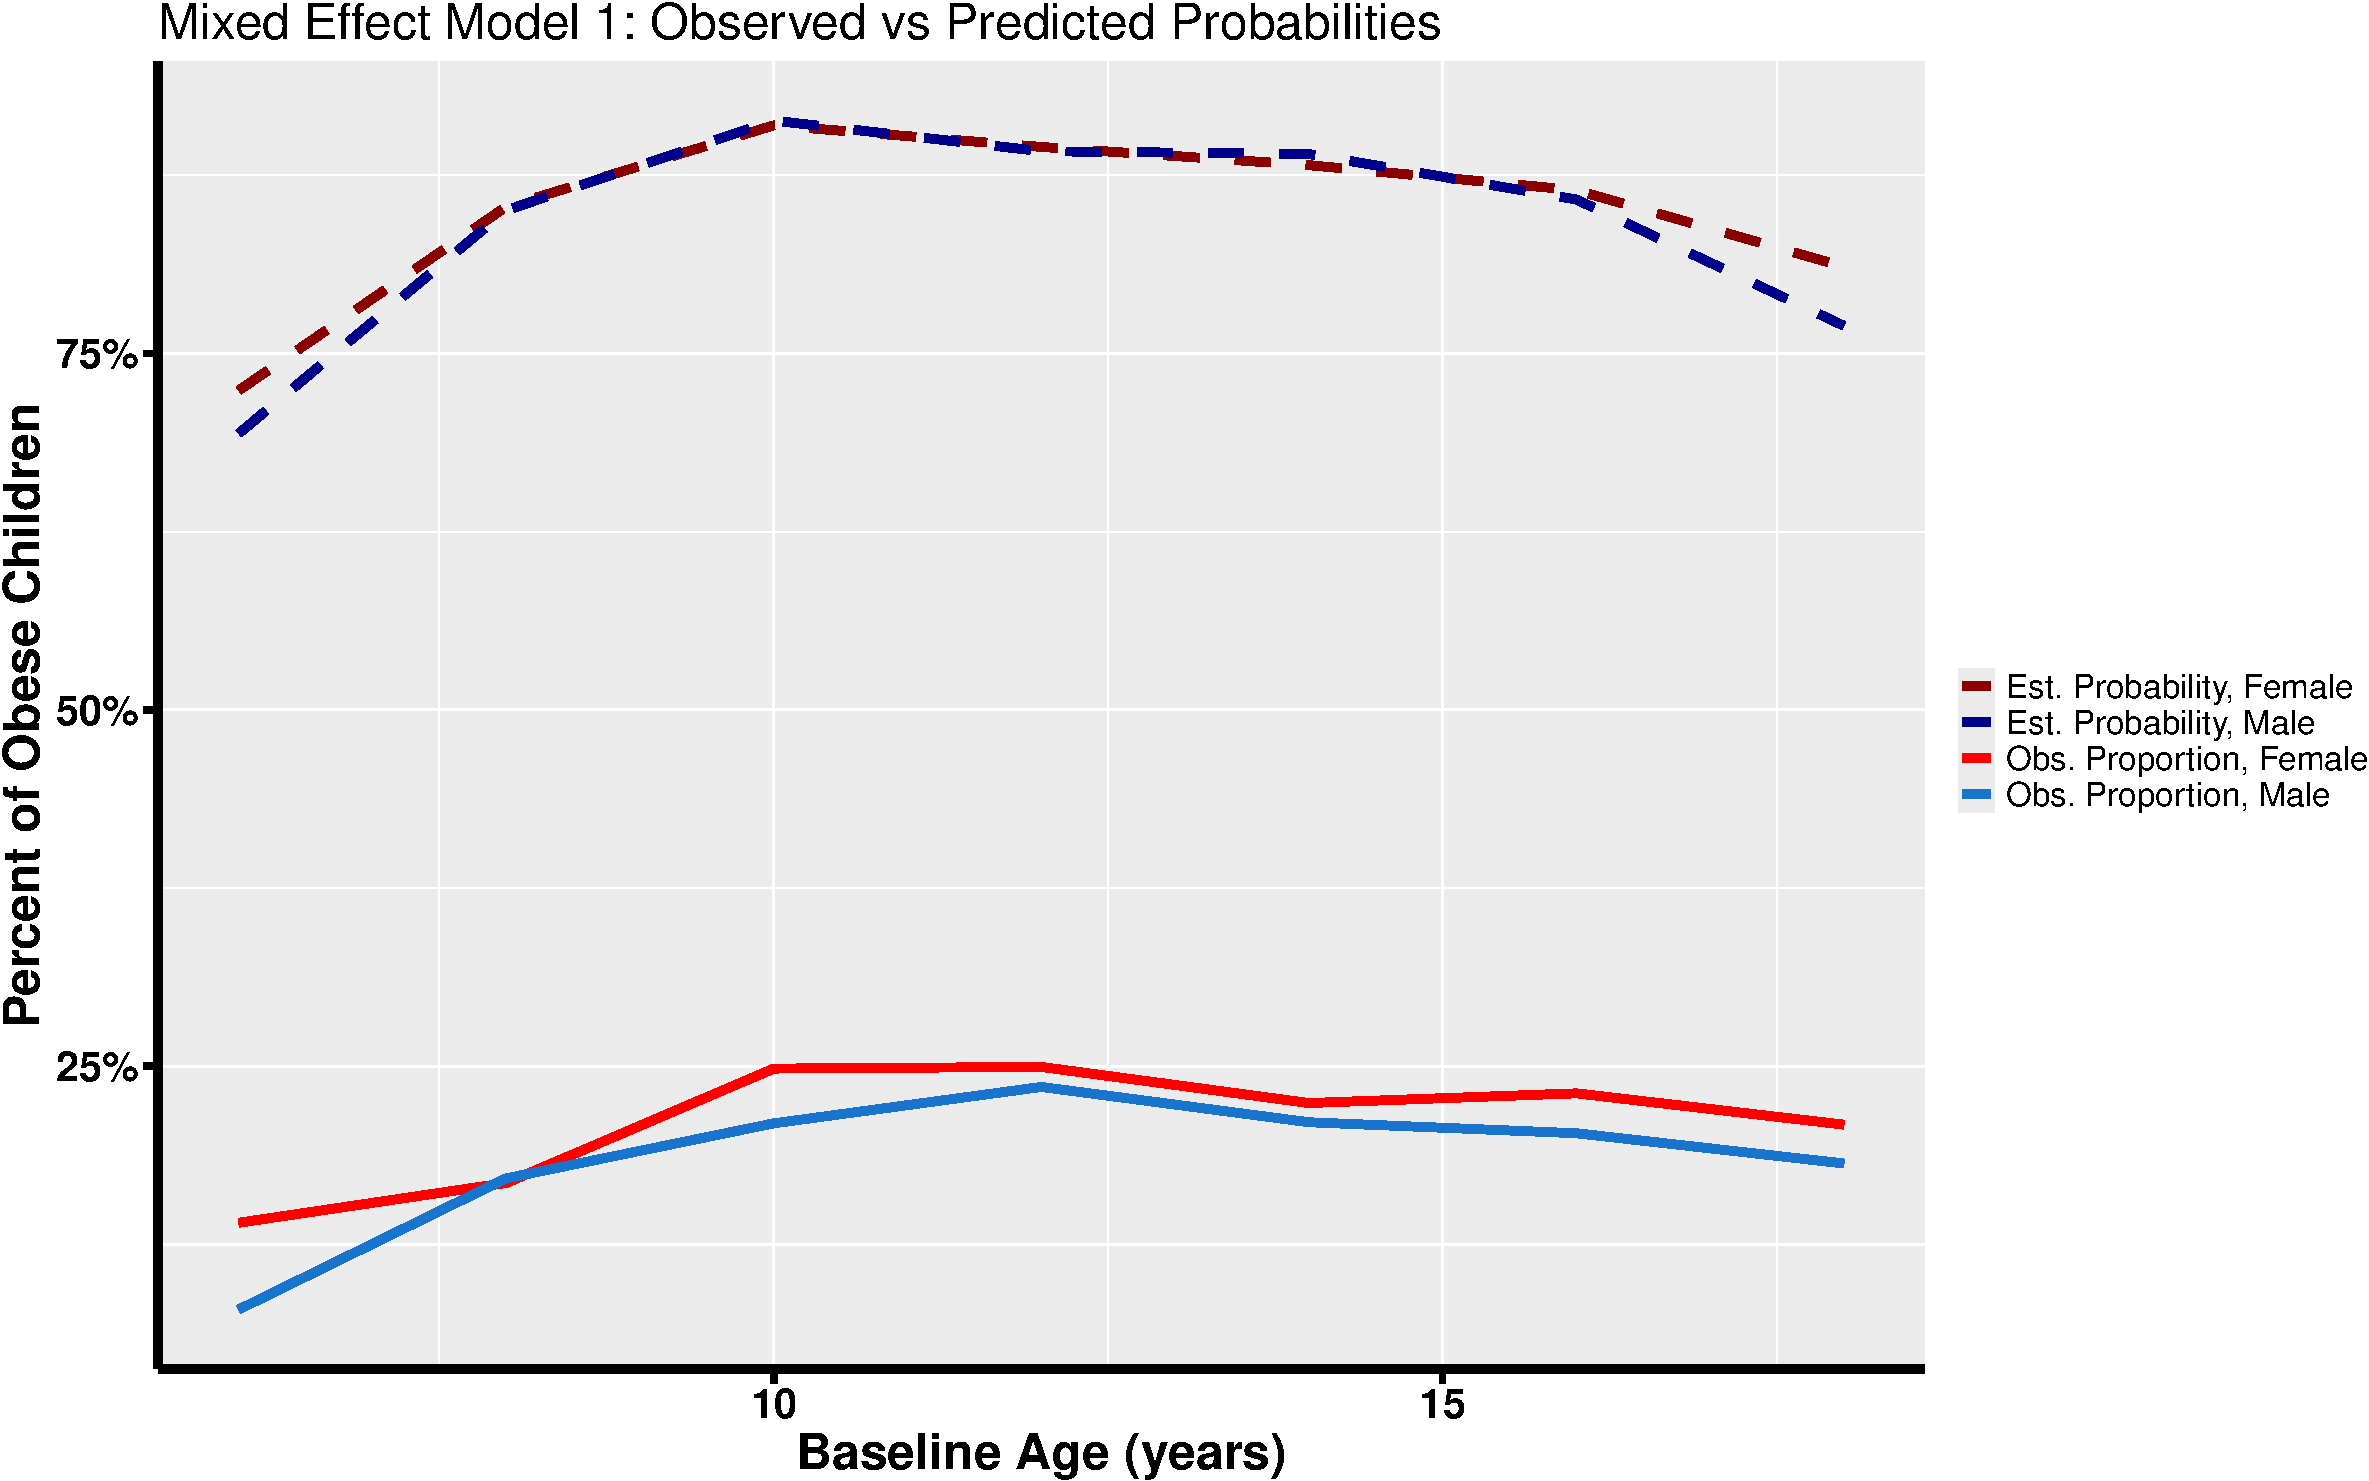
\includegraphics{Longi_noncontinuous_files/figure-pdf/unnamed-chunk-23-1.pdf}

}

\end{figure}

\begin{Shaded}
\begin{Highlighting}[]
\NormalTok{df }\OtherTok{\textless{}{-}} \FunctionTok{data.frame}\NormalTok{(}\AttributeTok{x =} \FunctionTok{rep}\NormalTok{(df\_models[, }\StringTok{"Age"}\NormalTok{], }\AttributeTok{times =} \DecValTok{4}\NormalTok{), }\AttributeTok{y =} \FunctionTok{c}\NormalTok{(df\_models2[, }\StringTok{"Est\_Female4"}\NormalTok{],}
\NormalTok{    df\_models2[, }\StringTok{"Est\_Male4"}\NormalTok{], df\_models2[, }\StringTok{"Obs\_Female"}\NormalTok{], df\_models2[, }\StringTok{"Obs\_Male"}\NormalTok{]),}
    \AttributeTok{group =} \FunctionTok{rep}\NormalTok{(labels, }\AttributeTok{each =} \DecValTok{7}\NormalTok{))}

\NormalTok{df }\SpecialCharTok{\%\textgreater{}\%}
    \FunctionTok{ggplot}\NormalTok{() }\SpecialCharTok{+} \FunctionTok{geom\_line}\NormalTok{(}\FunctionTok{aes}\NormalTok{(x, y, }\AttributeTok{color =}\NormalTok{ group, }\AttributeTok{linetype =}\NormalTok{ group), }\AttributeTok{linewidth =} \DecValTok{2}\NormalTok{) }\SpecialCharTok{+}
    \FunctionTok{theme}\NormalTok{(}\AttributeTok{axis.line =} \FunctionTok{element\_line}\NormalTok{(}\AttributeTok{colour =} \StringTok{"black"}\NormalTok{, }\AttributeTok{linewidth =} \DecValTok{2}\NormalTok{), }\AttributeTok{text =} \FunctionTok{element\_text}\NormalTok{(}\AttributeTok{size =} \DecValTok{20}\NormalTok{),}
        \AttributeTok{axis.text =} \FunctionTok{element\_text}\NormalTok{(}\AttributeTok{colour =} \StringTok{"black"}\NormalTok{, }\AttributeTok{size =} \DecValTok{20}\NormalTok{, }\AttributeTok{face =} \StringTok{"bold"}\NormalTok{), }\AttributeTok{axis.title =} \FunctionTok{element\_text}\NormalTok{(}\AttributeTok{size =} \DecValTok{24}\NormalTok{,}
            \AttributeTok{face =} \StringTok{"bold"}\NormalTok{), }\AttributeTok{axis.ticks.length =} \FunctionTok{unit}\NormalTok{(}\FloatTok{0.25}\NormalTok{, }\StringTok{"cm"}\NormalTok{), }\AttributeTok{axis.ticks =} \FunctionTok{element\_line}\NormalTok{(}\AttributeTok{colour =} \StringTok{"black"}\NormalTok{,}
            \AttributeTok{linewidth =} \FloatTok{1.5}\NormalTok{)) }\SpecialCharTok{+} \FunctionTok{scale\_color\_manual}\NormalTok{(}\AttributeTok{name =} \StringTok{" "}\NormalTok{, }\AttributeTok{labels =}\NormalTok{ labels, }\AttributeTok{values =} \FunctionTok{c}\NormalTok{(}\StringTok{"darkred"}\NormalTok{,}
    \StringTok{"darkblue"}\NormalTok{, }\StringTok{"red"}\NormalTok{, }\StringTok{"dodgerblue3"}\NormalTok{)) }\SpecialCharTok{+} \FunctionTok{scale\_linetype\_manual}\NormalTok{(}\AttributeTok{name =} \StringTok{" "}\NormalTok{, }\AttributeTok{labels =}\NormalTok{ labels,}
    \AttributeTok{values =} \FunctionTok{c}\NormalTok{(}\StringTok{"dashed"}\NormalTok{, }\StringTok{"dashed"}\NormalTok{, }\StringTok{"solid"}\NormalTok{, }\StringTok{"solid"}\NormalTok{)) }\SpecialCharTok{+} \FunctionTok{scale\_y\_continuous}\NormalTok{(}\AttributeTok{labels =}\NormalTok{ percent) }\SpecialCharTok{+}
    \FunctionTok{ggtitle}\NormalTok{(}\StringTok{"Mixed Effect Model 2: Observed vs Predicted Probabilities"}\NormalTok{) }\SpecialCharTok{+} \FunctionTok{ylab}\NormalTok{(}\StringTok{"Percent of Obese Children"}\NormalTok{) }\SpecialCharTok{+}
    \FunctionTok{xlab}\NormalTok{(}\StringTok{"Baseline Age (years)"}\NormalTok{)}
\end{Highlighting}
\end{Shaded}

\begin{figure}[H]

{\centering 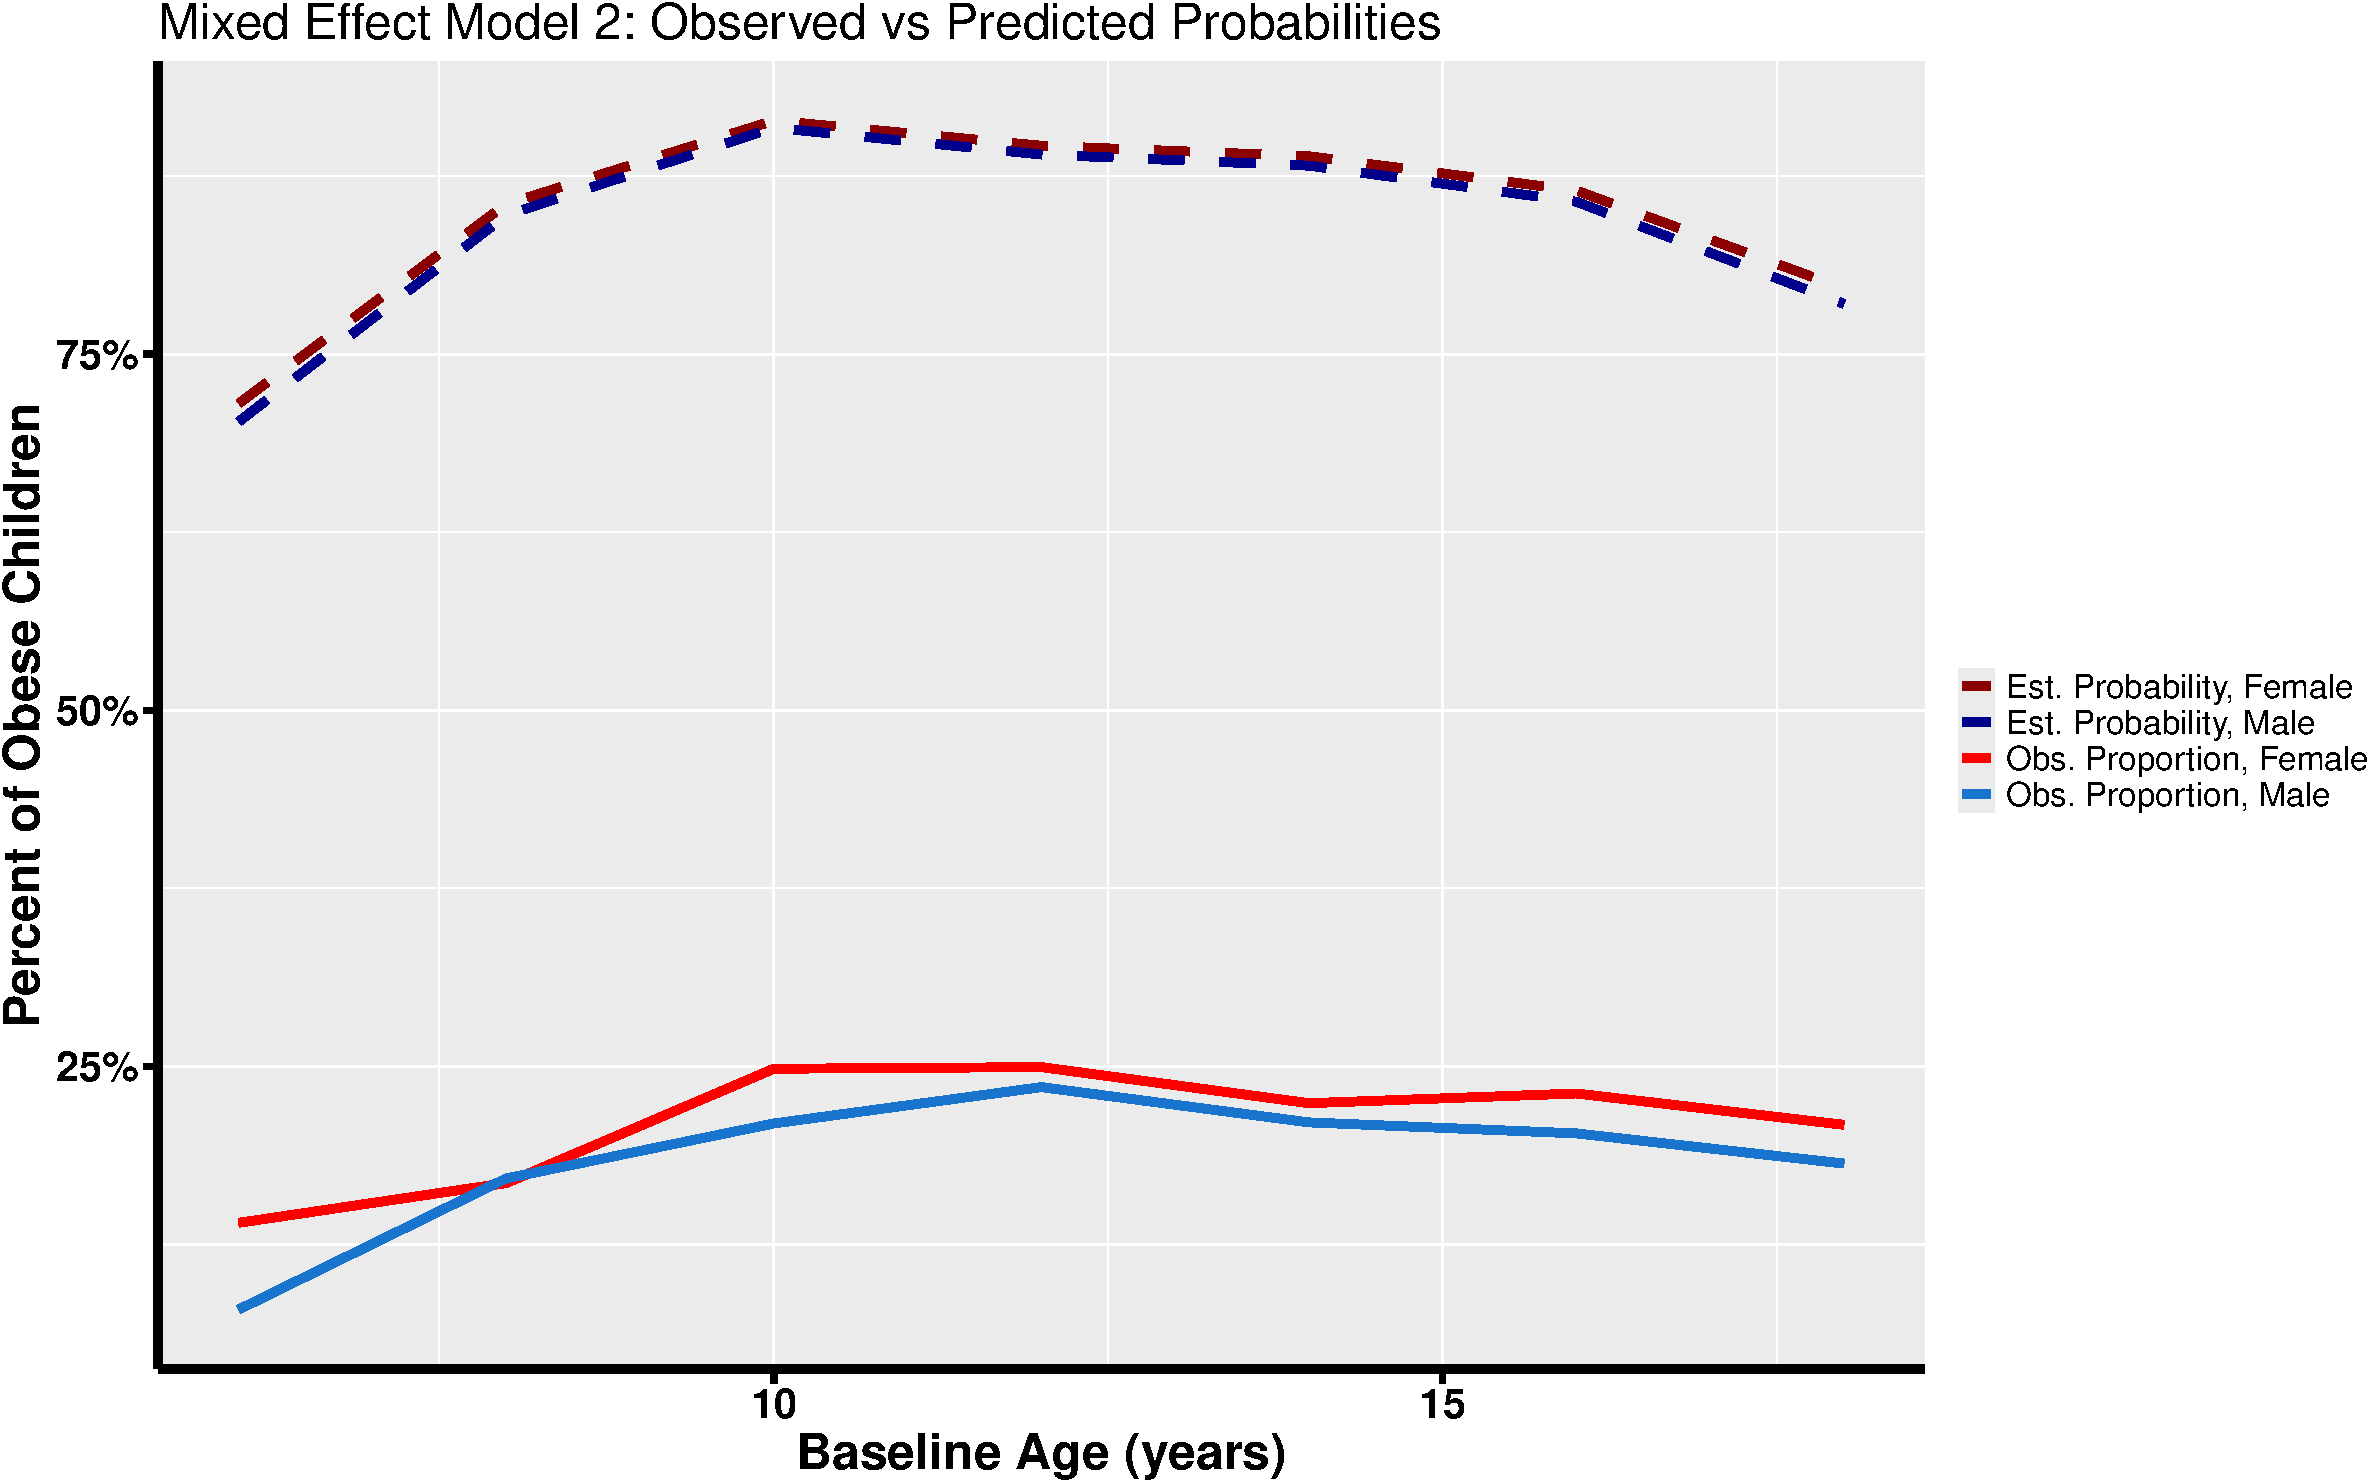
\includegraphics{Longi_noncontinuous_files/figure-pdf/unnamed-chunk-24-1.pdf}

}

\end{figure}

\hypertarget{binary-outcome}{%
\section{Binary Outcome}\label{binary-outcome}}

\hypertarget{count-outcome}{%
\section{Count Outcome}\label{count-outcome}}

\hypertarget{sec-longi-missingdata}{%
\chapter{Missing Data}\label{sec-longi-missingdata}}



\printindex

\end{document}
